\chapter[Study 3: Application of SPARC to Tutoring]{Study 3: \\Application of SPARC to Tutoring}\label{chap:tutoring}
\glsresetall
\graphicspath{{images/tutoring/}}

\begin{framed}
	\textbf{Key points:}
	
	\begin{itemize}
		\item Design of an experiment to test \acrshort{sparc} in an educational application with children.
		\item Design and use of a new learning algorithm adapted from nearest neighbours to teach quickly and efficiently in an online fashion.
		\item Between participants study involving 75 children comparing 3 conditions: a passive robot, a supervised robot and an autonomous robot.
		\item Psychology PhD student teaching the supervised robot using \acrshort{sparc}.
%		\item No significant differences of child learning between conditions.
		\item Children behaved similarly with the autonomous and supervised robot, and differently with the passive robot.
		\item Demonstrate  the application of \acrshort{sparc} to teach a robot an action policy online to interact with humans in a social environment which is complex, indeterministic, high dimensional and multimodal.
	\end{itemize}
\end{framed}

Parts of the work presented in this chapter have been published verbatim in \cite{senft2017toward} and \cite{senft2018robots} and an additional publication is under review. The final publications are available from AAAI, EPFL via:
\begin{itemize}
	\item \url{https://aaai.org/ocs/index.php/FSS/FSS17/paper/view/16011}.
	\item \url{https://r4l.epfl.ch/files/content/sites/r4l/files/HRI2018/proceedings_2018/paper4.pdf}.
\end{itemize} 

%Technical contribution in this chapter: the author extended code the freeplay sandbox, see \url{https://github.com/freeplay-sandbox/} and forks.

\newpage

\section{Motivation}

Chapters~\ref{chap:woz} and~\ref{chap:control} tested the \gls{sparc} in interactions between robots or in a virtual world but not for \gls{hri} as it was intended to be used. As such, this Chapter addresses the thesis of this research and evaluates if \gls{sparc} can efficiently be used to teach a robot an interactive behaviour for real human-robot interactions. \gls{hri} in the wild typically occurs in constrained but underspecified environments where social behaviours play an important role. Teaching a robot in such an environment is a challenge as the state and action spaces are high-dimensional, the environment is not deterministic and the interaction takes place in continuous time and is multimodal. Additionally, the social side is fundamental as it impacts the flow and the success of the interaction and makes \gls{hri} a high-stakes environment.%~\citep{belpaeme2012multimodal}. %This would be one of the first times humans have been used to teach online a robot to interact with humans.

This study took place in the context of robot tutors for children in education, more precisely in the context of teaching about food chains. Tutoring has be selected as this framework is widely used in \gls{hri}, and which provides opportunities for a rich and complex interaction between a child and a robot~\citep{leyzberg2012physical,kennedy2015robot}. This scenario and the code used control the robot and define the educational application are based on \cite{lemaignan2017free} but have been adapted to provide a new teaching task (teaching game and protocol), a knowledge test, a robot controller, a learning algorithm and an interface with the teacher supporting \gls{sparc}.

%This study aims to explore if \gls{sparc} can be used to teach a robot an efficient action policy. As such, three conditions have been compared: a passive robot (not providing any support), a supervised robot (learning from a human teacher and supporting the child) and an autonomous robot (applying the learned behaviour). These three conditions, with the passive robot as a control condition, allow us to study both the teaching process and the efficiency of the taught behaviour when being executed without supervision.

\section{Scope of the Study} \label{sec:tutoring_scope}

The main goal of this study was to directly explore the thesis proposed in this research work: ``A robot can learn to interact meaningfully with humans in an efficient and safe way by receiving supervision from a human teacher in control of the robot's behaviour''. This thesis can be divided into two parts: ``a robot can learn safely by receiving supervision from a human teacher'' and ``after learning, such a robot would have a meaningful interaction with humans autonomously''. To address these two statements, a study comparing three conditions was designed (passive robot, supervised robot and autonomous robot). The study was composed of two main elements: four rounds of an educational game children played with the robot and where they could gain knowledge about food chains, and three tests outside of the game to evaluate the knowledge children gained when playing. During the game, the robot could provide feedback, hints and supporting messages to the child participating depending on the condition. 

The objective of the study was to explore whether the robot could be taught to provide an efficient tutoring support to the children during this game, 
%For this study, the goal of the interaction is learning about food chains by exploring a specific food web (interconnections between multiple food chains) in an educational game. The child plays a game on the Sandtray where they can move animals to discover the interactions between them. Learning is evaluated by a test before, between and after the rounds; and the robot leads the child through the study and can, depending of the condition, support them during the game.
%This study was focused on providing a robot with an efficient tutoring behaviour, 
and examining how this autonomous behaviour would compare to no behaviour (passive) and to human-controlled behaviour. As such, three conditions were required: a control condition (with a passive robot), a supervised condition (where the robot was taught) and an autonomous condition (to evaluate the learned behaviour). In both the supervised and the autonomous conditions, the robot was active during the game and provided support to the child.

%to prevent confounds about novelty effect and potential excitements due to the presence of the robot, the control condition maintained the robot present through all the interaction. In this control, `passive', condition, the robot led the child through the study as in the other conditions, but was not interacting with the child during the educational game. This condition provided a benchmark against which the other conditions were compared to evaluate the `meaningfulness' and efficiency of the robot's behaviours. In the second condition, the `supervised' condition, the robot was supervised and taught by a human teacher using \gls{sparc}. This condition was the one in which the robot learned, and was used to evaluate the impacts of the principles underlying \gls{sparc} when teaching a robot to interact with humans. Lastly, in the `autonomous' condition, the robot applied the learnt policy to interact without supervision with the children. This condition aimed at exploring the similarity between the autonomous policy and the supervised one, and evaluating if the teaching from the human was successful. And, as the robot needed to have completed its learning before interacting alone, this condition was run only after the supervised condition was completed.

As such, there were four experimental hypotheses:
\begin{itemize}
	\item [H1] In the supervised condition, the teacher will be able to ensure an appropriate robot behaviour whilst teaching.
	\item [H2] The autonomous robot will be able to interact socially and efficiently during the game and maintain the child's engagement during the learning task.
	\item [H3] An active robot (supervised or autonomous) supports child learning: the learning gain in passive condition will be inferior to the learning gain in autonomous condition, which will be inferior to the learning gain in supervised condition.
	\item [H4] Using \gls{sparc}, the workload on the supervisor decreases over time: the number of corrected actions and the number of actions selected  by the teacher decrease with practice, while the number of correct proposed actions increases.
\end{itemize}

H3 is motivated by the idea that the humans possess knowledge which should help the child to learn more from the game. By learning this knowledge, the autonomous robot should be able to partially replicate this effect, but without being able to match it due to lack of learning time or limits of the world representation or algorithm.

\section{Methodology}

\subsection{Participants}

Children from five classrooms across two different primary schools in Plymouth were recruited to take part in the study. As both schools have an identical OFSTED evaluation (indicating that they provide similar educational environment), all the children were combined into a single pool of participants. Full permission to take part in the study and be recorded on video was acquired for all the participants via informed consent from parents. In total, 119 children participated in the study, however 75 children were included in the final analysis. 14 participants took part in two pilot versions, with previous versions of the game or the protocol. 9 participants were excluded due to a breach in protocol or technical error (such as freezing of the tablet due to an imperfect kernel version or children refusing to continue the interaction). Additionally, children with special needs were encouraged to participate but were not included in the analysis (N=8). In the end, 25 participants per condition were included (N=75; age: \textit{M}=9.4, \textit{SD}=0.72; 37 female). The remaining 13 children in the classrooms interacted in pairs or alone to ensure that all children were able to interact with the robot within the time-frame the school provided and keep a balanced number of participants per condition. 

\subsection{Apparatus}

Similarly to the study presented in Chapter~\ref{chap:woz}, this study is based on the Sandtray paradigm~\citep{baxter2012touchscreen}: a child interacts with a robot via a large touchscreen located between them. By interacting with the touchscreen and the robot, the child is expected to gain knowledge or improve some skills. Additionally, a teacher can use a tablet to control and teach the robot in the `supervised' condition (cf. Figure~\ref{fig:tutoring_setup}). This type of triadic interaction is typical of the interactions we considered when framing this research (cf. Figure~\ref{fig:intro_setup}): a human knows how the robot should behave and can supervise it and teach it how to interact with another human \textit{in situ} by using \gls{sparc}.

%We desire an efficient behaviour for the robot in the application interaction (i.e. child tutoring) and a human teacher has knowledge about how the robot should behave and can transfer it to the robot .

\begin{figure}[ht]
	\centering
	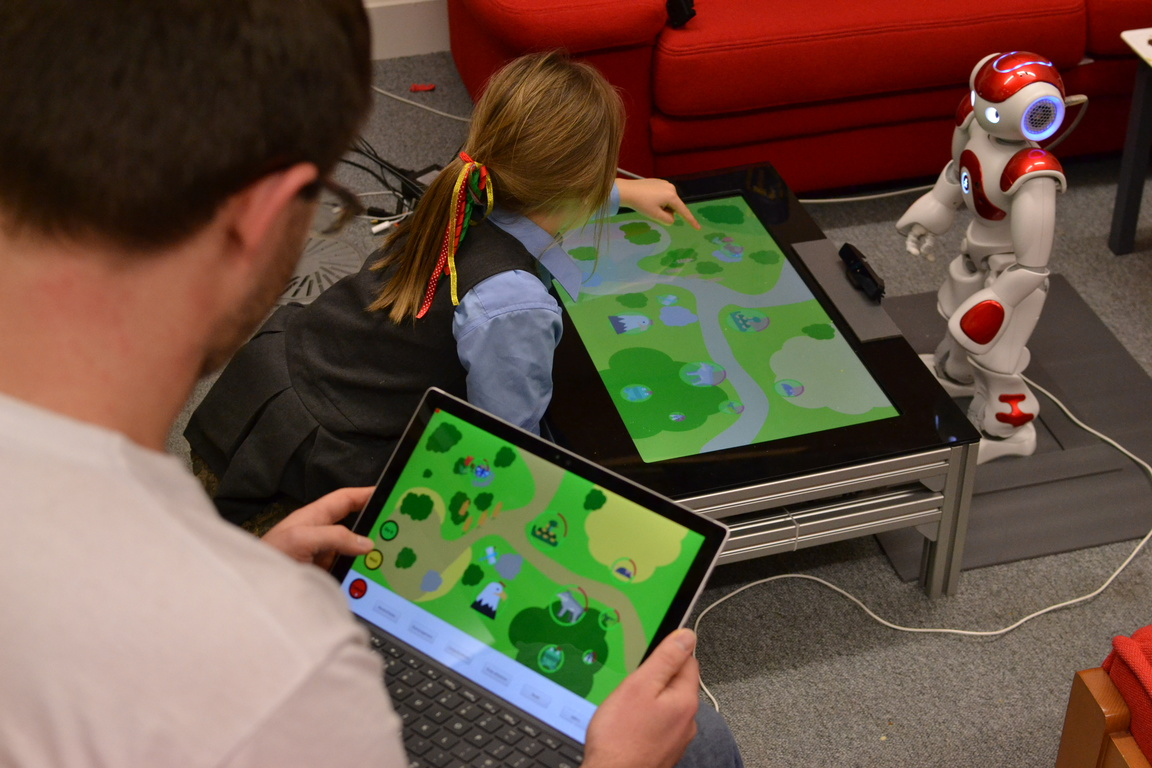
\includegraphics[width=1\textwidth]{setup.jpg}
	\caption{Setup used in the study: a child interacts with the robot tutor, with a large touchscreen sitting between them displaying the learning activity; a human teacher provides supervision to the robot through a tablet and monitors the robot learning.}
	\label{fig:tutoring_setup}
\end{figure}

\subsection{Food Chain Game}

The main learning activity to teach the child about food chains is a game composed of ten interactive animals (a mouse, a grasshopper, an eagle, a frog, a snake, a fly, a wolf, a small bird, a butterfly and a dragonfly) which can be moved by the children and three types of plants (4 wheat plants, 4 apples and 3 flowers, for a total of 11 plants) that are static and are not moving during the game. Animals have energy which decreases over time and they have to eat to increase their energy levels. Figure~\ref{fig:tutoring_game} presents an example of the game screen in the middle of a round. Animals only move if the child or the robot moves them and can eat or be eaten when the child put them in contact with another animal or a plant. The child is instructed to keep the animals alive as long as possible, and consequently has to feed the animals by moving them to their food. By feeding the animals, children can learn the animals' diet. 

\begin{figure}[ht]
	\centering
		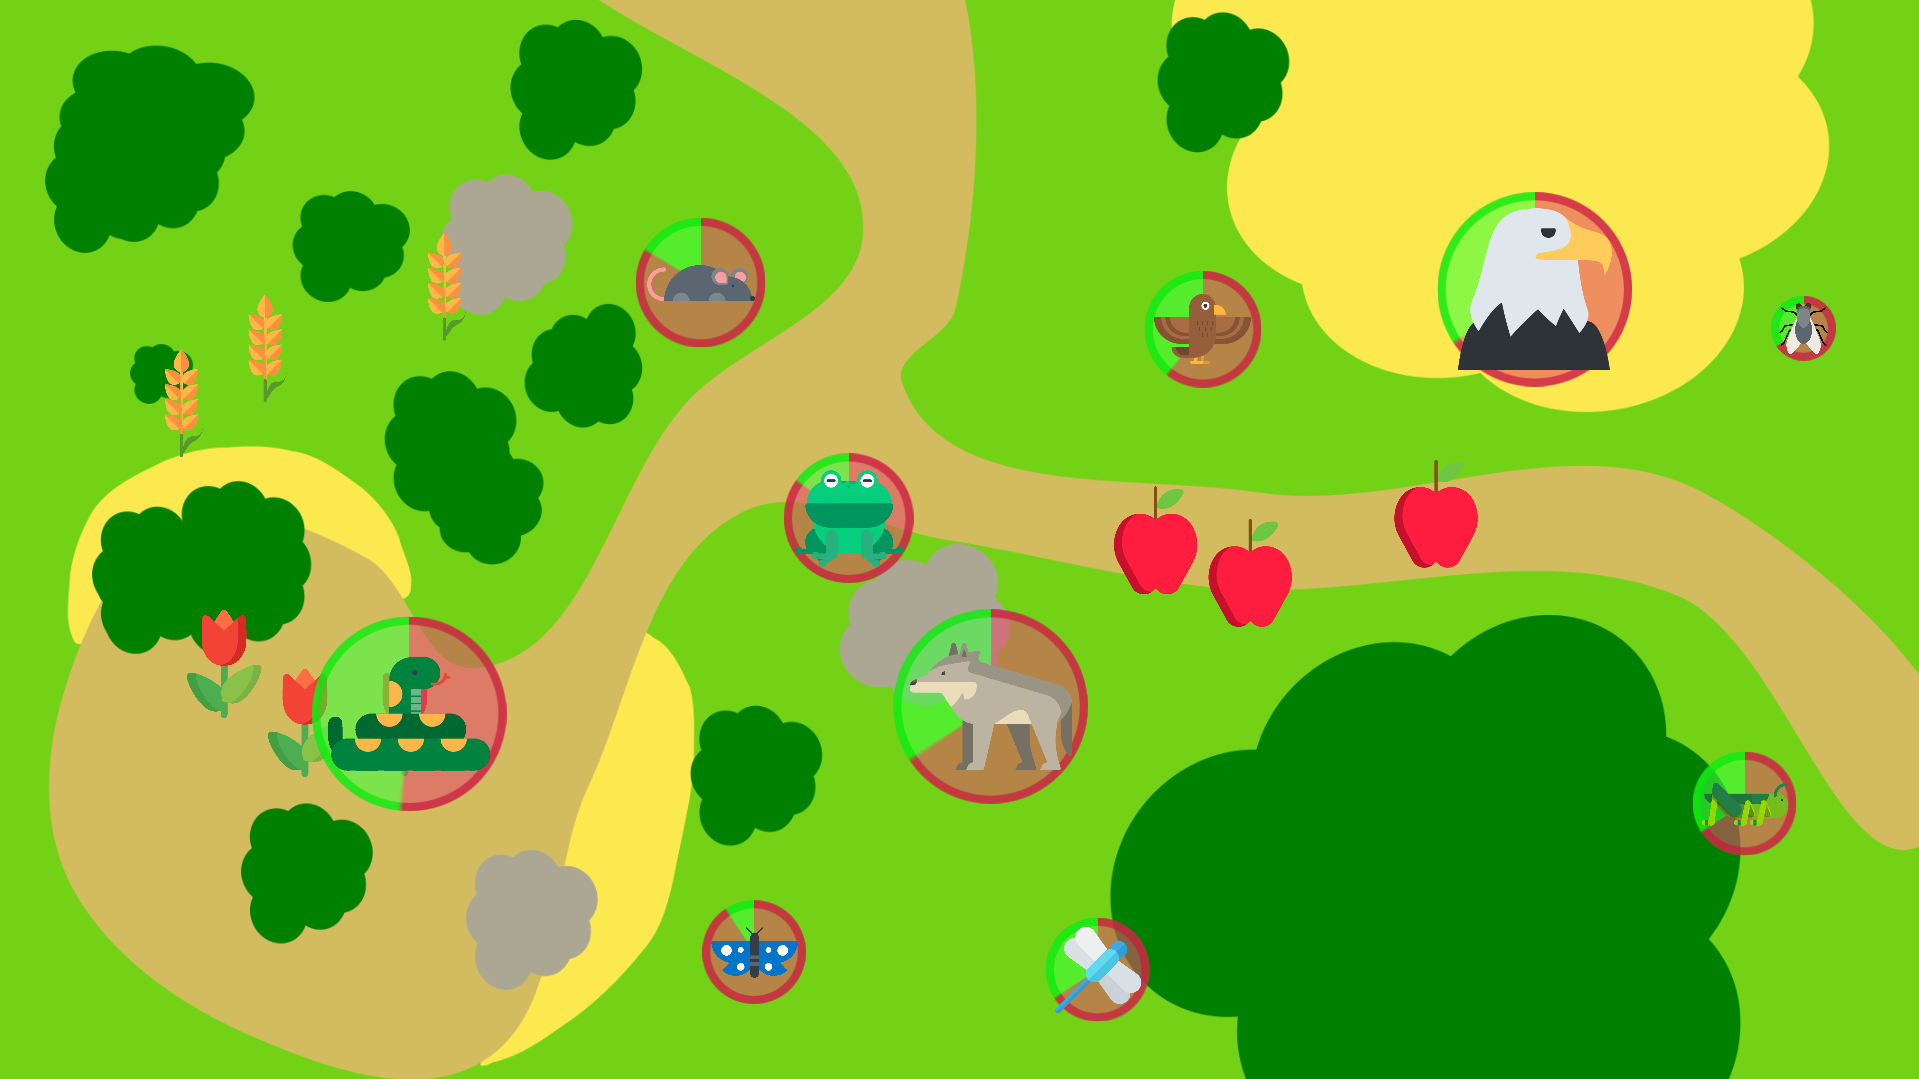
\includegraphics[width=1\textwidth]{game.png}
		\caption{Example of the game. Animals have energy in green and have to eat plants or other animals to survive. The child's task is to keep animals alive as long as possible.}
		\label{fig:tutoring_game}
\end{figure}

\subsection{Robot Behaviour} \label{sec:tuto_robot}
In each condition, the robot leads the child through the interaction by: asking them to fill in the demographic questions, explaining the tutorial and guiding them through the test steps. During the game, depending on the condition, the robot can execute actions to provide hints and support to the child. The robot has access to five types of actions:
\begin{itemize}
	\item Movements: moving any animal \emph{to}, \emph{close to} or \emph{away from} any items (animal or plant) - the robot points to an animal, the image of a robot hand appears on the screen and moves the animal's image, synchronised with a physical gesture of robot and a verbal description of the action (e.g. "The eagle needs help getting close to the mouse").
	\item Drawing attention: the robot points to an item and gives a verbal reminder to the child (e.g. "Don't forget the frog").
	\item Reminding rules: the robot says one of 5 sentences describing the game's rules (e.g. "Move the animals to feed them" or "Feed animals with a low energy").
	\item Congratulation: the robot provides congratulations (e.g. "Well done").
	\item Encouragement: the robot provides encouragement (e.g. "You can do it").
\end{itemize}
Considering all the possible combinations of actions and items, the total number of actions equals 655. Additionally, to prevent the robot's behaviour from being repetitive, each action has multiple possible utterances, and a random one, not used recently, is spoken by the robot when an action is executed. When the robot is not acting, it simply sways slightly to simulate a breathing motion and follows the child's face. 

This set of actions was designed to be multimodal: involving verbal utterances, pointing gestures and movements on the game and to cover different ranges of tutoring behaviours. Some actions, such as encouragement and congratulations, are mostly social and do not provide much information on the game. Others are only hints such as drawing attention. And finally the last ones: motions and reminding rules, provide game content, but their timing is related to game events or social norms (such as turn taking). In summary, this action set aims to allow the robot to express different types of tutoring behaviour: from providing motivation and general information about the game's goal to giving hints regarding which animals the child should focus on or information about what an animal eats. %This set of actions constitutes a substantial range of tutoring behaviours a human teacher would employ.

The goal of the interaction is to have the child, not the robot, play the game. Therefore, the robot can only move the animals to location on the game, and these motions do not trigger feeding events. Only the child can feed the animals by moving them in contact of a food source, hence, all the events and real changes in the game are created by the child. 
\subsection{Control Architecture}\label{sec:tuto_arch}

The code used to create the game and control the robot is an adaptation of the Freeplay Sandbox~\citep{lemaignan2017free}. Original sources are available online\footnote{\url{https://github.com/freeplay-sandbox}} as well as the code used for this study\footnote{\url{https://github.com/emmanuel-senft/freeplay-sandbox-qt/tree/food-chain}
	
\url{https://github.com/emmanuel-senft/freeplay-sandbox-ros-sparc/tree/task}
	
\url{https://github.com/emmanuel-senft/freeplay-sandbox-qt-supervisor}}.

The control architecture is adapted from \cite{lemaignan2017free} and a simplified schematic is presented in Figure~\ref{fig:tutoring_arch}. All nodes are communicating through the \gls{ros} \citep{quigley2009ros} and the communication with the robot is done through NAOqi, Softbank's operating system for the Nao robot. The tool rosbag\footnote{http://wiki.ros.org/rosbag} is used to collect data throughout the interaction and the analysis of the child's head gaze is performed using gazr~\citep{lemaignan2016real}.

\begin{figure}[ht]
	\centering
	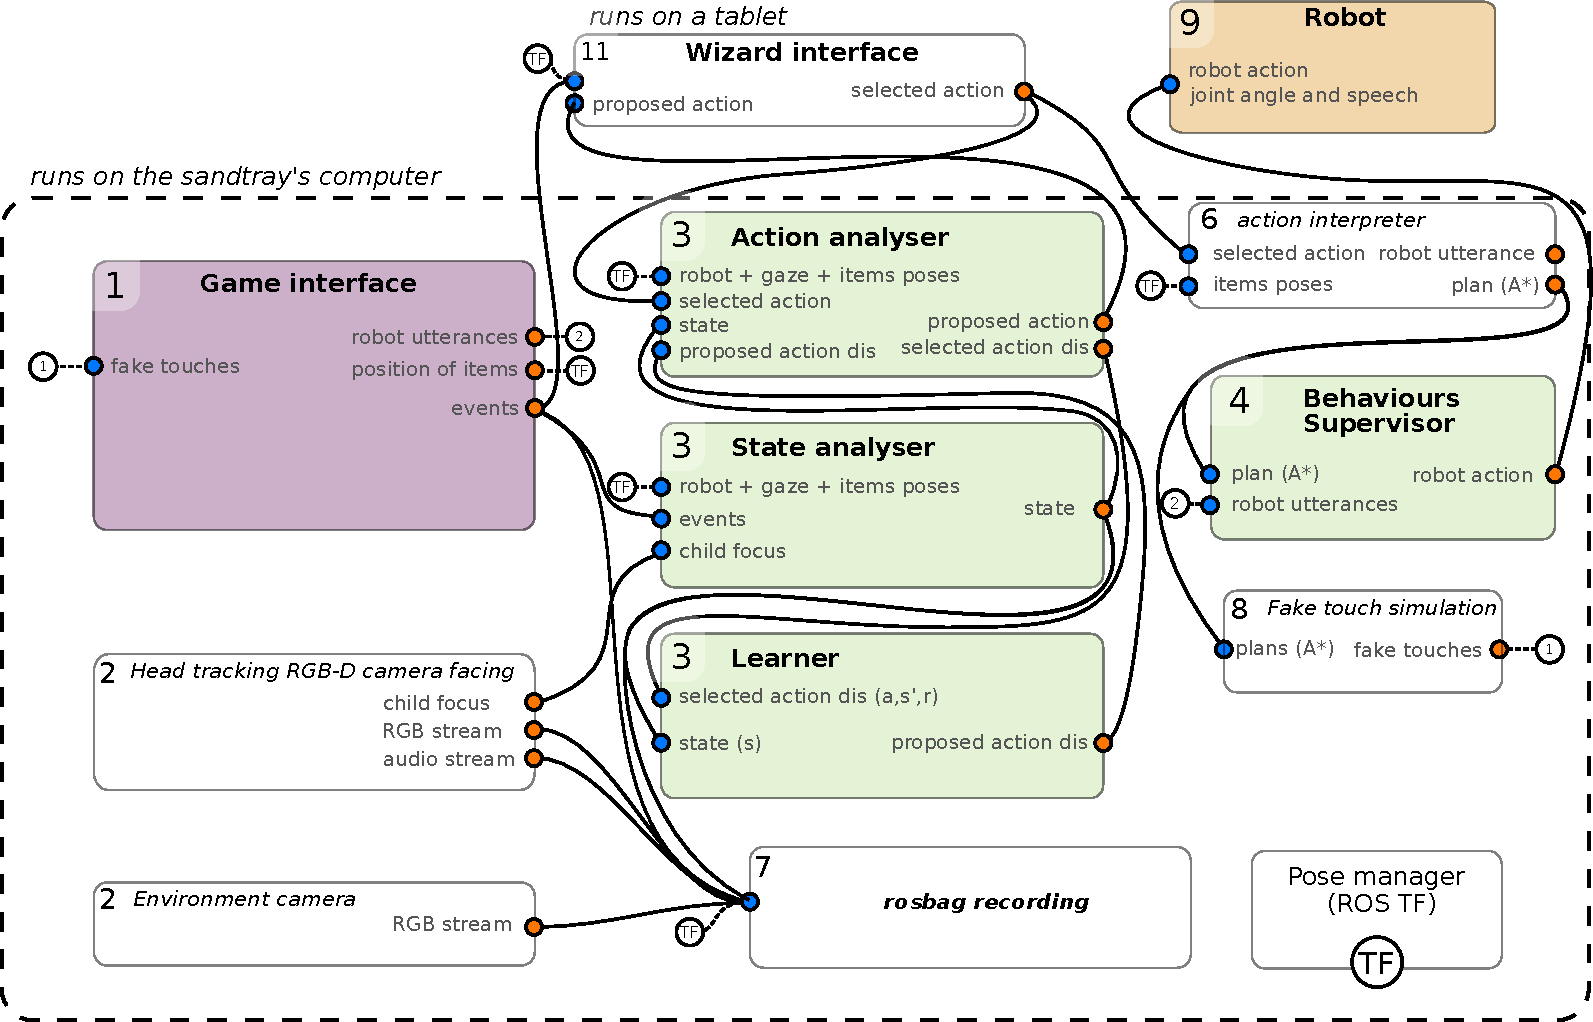
\includegraphics[width=1\textwidth]{architecture.pdf}
	\caption{Simplified schematics of the architecture used to control the robot. In addition, all the topics related to the actions are recorded using rosbag. (Figure adapted from \citealt{lemaignan2017free}).}
	\label{fig:tutoring_arch}
\end{figure}

%Two worlds are cohabiting, the continuous world (as perceived by the child and the teacher) and the discrete world (as perceived by the algorithm). In the continuous world, actions are 

The control architecture can be divided into 6 main parts.

\paragraph{1/ The Game Interface} is responsible for displaying the game and the test on the touchscreen and generating game related data used to control the robot. The interface is coded in QML, a markup language for creating user interface-centric applications, and a ROS-QML bridge adapted from the one in \cite{lemaignan2017free} provides a way to send and receive message from ROS, thus connecting the interface with the rest of the control architecture.

\paragraph{2/ The State Analyser} collects data from the interface and camera and from these continuous data and events generates a 210-dimensional state used for the learning (cf. Section~\ref{sec:tuto_state}). The state is generated at 2Hz, the frequency used to update the animals life due to the hunger.

\paragraph{3/ The Wizard Interface} is the tool used by the teacher to control and teach the robot. The teacher can use it to send actions to the robot to execute (such as movements or verbal feedback) and react to propositions from the algorithm. Two precisions should be added. First, on the interface, the teacher do not select the discrete actions for motions described in Section~\ref{sec:tuto_robot}, they create continuous actions, such as moving an animal from a position A to B and select the items on the screen required for interpreting this action. The exact discrete action among the 655 presented earlier is inferred by the action analyser and used by the learner. Additionally, by highlighting items on the screen, the teacher can inform the algorithm about the features relevant to the selection of this action in that state. Each time the teacher selects an action or react to a proposition, it sends to the action analyser a message containing the continuous action (motion of an animal from A to B, or a string informing the type of action for the verbal feedback), the features relevant to the selection (as a list of string of highlighted items) and a rewards related to the acceptance or refusal of the action. Additional details can be found in Section~\ref{sec:tuto_woz}. 

In the autonomous condition, the wizard interface is replaced by a node on the sandtray automatically accepting the actions proposed by the learner after a short delay.

\paragraph{4/ The Action Analyser} transforms the continuous actions from the teacher (such as moving an animal from point A to B) into discrete actions (moving an animal to, close to or away from an item). By using the features selected by teacher on the interface and the movements if applicable, this node infers a discrete action (a number from 0 to 654) and a state mask (informing the algorithm of the relevant dimensions of the state space) that are sent with the reward to the algorithm for learning (cf. Section~\ref{sec:tuto_algo}). In case of ambiguity (for example if no target is selected when moving an animal), the action analyser will assume that the target was the closest item to arriving position and will automatically add this feature to infer the action and the state mask. Similarly, this nodes also transforms discrete actions from the algorithm into continuous actions to submit to the teacher through the interface: for example finding a location (set of coordinate on the screen) where an animal should go to be moved close to another item.

\paragraph{5/ The Action Interpreter and 6/ the Behaviour Supervisor} take the actions selected by the teacher and transform them in motor commands, fake touches on the screen and verbal utterances for the robot.

\paragraph{7/ The Learner} is responsible for having the algorithm propose actions and learn. It takes as input the state space at each time step and actions selected by the teacher (action number, state mask and reward) and store corresponding instances in memory. Each time the learner receives a state, it compares it instances in memory and proposes an action if appropriate (cf. Section~\ref{sec:tuto_algo}).
%It should be noted that in order to learn actions the algorithm used a discrete actions space consisting of the 655 actions defined in Section~\ref{sec:tuto_robot}. On the other hand, for the teacher, movement actions are continuous, they can be selected by choosing an animal and a moving to a destination while highlighting relevant features to clarify the action if needed or help the learning. The action analyser has the task of converting the actions from one world to another: interpreting movements from the teacher as discrete actions for the algorithm and transforming the discrete actions from the algorithm to continuous action for the teacher and the game.

\subsection{Environment Modelisation}

To learn and act autonomously, the robot has access to a representation of the state of the interaction and a set of actions it can perform. The algorithm aims at finding the ideal action for each possible state based on the teacher's commands.

\subsubsection{State}\label{sec:tuto_state}

Table~\ref{tab:tuto_state_space} presents the different dimensions composing the state the robot has access to. The state analyser is responsible to update and broadcast this state at 2Hz.

\begin{table}[ht]
	\centering
	\ra{1.4}
	\caption{Definition of each category of the state space.}
	\label{tab:tuto_state_space}
	\begin{tabularx}{\textwidth}{@{}L{.65}L{1.05}L{.15}L{2.15}@{}}\toprule
		Group & Name & \# & Description \\
		\midrule
		Game State & Distance Between Items & 155 & Normalised distance between the animals and each other animal and the plants\\
		& Items' Energy & 21 & Energy of the 21 items (10 animals and 11 plants)\\
		& Progress in the Game & 1 & 0.25 for 1st game to 1 for the last game\\ 
		Temporality & Robot Touches & 10 & Time since the robot touched each animal\\ %decay
		& Child Touches & 10 & Time since the child touched each animal\\ %accumulation
		& Task-Specific Events & 3 & Time since last feeding, failed interaction and death of an animal\\ %decay
		& Robot Actions & 5 & Time since last robot action of each type\\ %decay
		& Generic Last Actions & 2 & Time since any child touch and any robot action\\ %decay\accumulation
		Child state & Focus & 3 & Time of head gaze toward the robot, the screen and outside\\ %accumulation
		\bottomrule
	\end{tabularx}
\end{table}

All the state values in Table~\ref{tab:tuto_state_space} are bounded by [0,1]. Distances between items are normalised with the maximum possible distance (the diagonal of the screen), and as there are 10 animals and 11 plants this results in a total of 155 possible distances between animals and other items. To include a representation of the temporal aspects of the interaction, some dimensions of the state represent the time since events and two methods have been used to transform the time since an event to a value bounded between 0 and 1:
\begin{itemize}
	\item Accumulation: for the times since child touches and focus (effect being true or false).
	\item Decay: for robot actions and touches, and specific  events (temporally discrete events).
\end{itemize}

The accumulation corresponds to effects that can be true or not, and aims at representing how long this effect as been true or false. When the effect becomes true for accumulation, the state value is set to 0.5 and then increases at each step. When the condition becomes false, the value is set to 0.5 and then decreases at each step (cf. Algorithm~\ref{algo:tuto_acc} and Figure~\ref{fig:tuto_acc}). On the other hand, the decay refers to temporally discrete events, so only the time since the event is relevant. When the event happens the corresponding state value is set to 1 and then exponentially decreases by being multiplied by $e^{-\frac{1}{10}}$. That way events will have a `half-life' of 7 steps, which corresponds to 3.5 seconds, this aims to allow both short term reaction to an event (less than three seconds) and inform when an event did not happen in the last 10 or 20 seconds.


\begin{minipage}[t]{0.53\textwidth}
\begin{algorithm}[H]
	\While{Running}{
		\If{effect}{
			\If{$value < 0.5$}{
				$value = 0.5$
			}
			\Else{
			    $value = 1-(1-value) \cdot e^{-1/10}$
			}
		}
		\Else{
			\If{$value > 0.5$}{
				$value = 0.5$
			}
			\Else{
				$value = value \cdot e^{-1/10}$
			}	
		}
	}
	\caption{Formula to compute accumulation effects.}
	\label{algo:tuto_acc}
\end{algorithm}
\end{minipage}
\begin{minipage}[t]{0.47\textwidth}
		\centering
		\vspace{.1cm}
		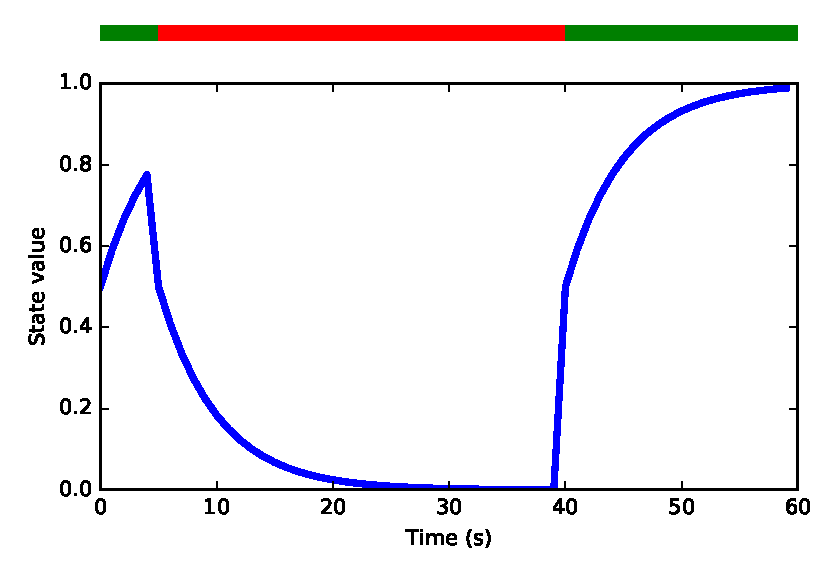
\includegraphics[width=1\textwidth]{accumulation.pdf}
		\captionof{figure}{Example of computation of accumulation. When the effect is true (green), the value increases, when the effect is false (red), the value decreases and the state is set to 0.5 when the effect's value changes.}
		\label{fig:tuto_acc}
\end{minipage}

Parts of the states are hardcoded, such as the task-specific events, generic last actions, focus and progress in the game. However, all the state dimensions related to the items (distance, energy and time since touches) are constructed on the fly. At start up, the state analyser node (cf. Figure~\ref{fig:tutoring_arch}), the node responsible for computing the state, receives a list of the interactive items and one of the static ones and creates the appropriate state with the corresponding dimensions. During the game, the state values are updated using events related to specific items (through their name) and hardcoded relation between task-specific events and state dimensions. 

%In summary, the state defines a generic way to represent the state of the interaction without any semantic hardcoded in it. All the dimensions are treated as equal and the algorithm has to infer the relation between state dimensions and action from the demonstrations.

\subsubsection{Actions}

Table~\ref{tab:tuto_actions_space} present the list of actions used for this activity.

\begin{table}[ht]
	\centering
	\ra{1.2}
	\caption{Definition of each category of the action space.}
	\label{tab:tuto_actions_space}
	\begin{tabularx}{\textwidth}{@{}lllX@{}}\toprule
		Type & Name & \# & Description \\
		\midrule
		Game & Move close & 210 &  Action moving any animal close to any item\\
		information & Move to & 210 & Action moving any animal to any item\\
		& Move away & 210 & Action moving any animal away from any item\\
		& Remind rules & 1 & Verbal utterance\\
		Social Feedback & Congratulation & 1 & Verbal utterance\\
		& Encouragement & 1 & Verbal utterance\\
		Hint & Attention & 21 & Drawing attention to any item\\
		Meta-level & Wait & 1 & Doing nothing\\
		\bottomrule
	\end{tabularx}
\end{table}

The total action space available is 655 actions. Each \emph{Move} action is composed of 200 possible actions the robot can execute, as we have a total of 10 animals which can be moved in relation to each other animal (9) and each plant (11), which results in 200 actions for moving close, 200 for moving to and 200 for moving away. It should be noted that technically 10 additional actions are available to the action analyser for each type of move (resulting in 210 actions per type of motion shown in Table~\ref{tab:tuto_actions_space}), but cannot be selected by the teacher (moving animals to/close to/away from themselves). However, as the learning algorithm is instance based and only uses the demonstration from the teacher, this does not impact the learning. 

%In the same way as the state definition, this action space has been selected to be general to many activities including movable and immobile images. 
%The action interpreter node selects the precise utterance to join to an action, and this node would have to be modified when adapting to a new activity. However, similarly to the state, the actions related to items are generated at run time, and could be adapted to another activity with minimal or no change of the code. 

%\ES{discuss the fact that limited semantic interpretation is used to define the action space - many not relevant actions, but even without this semantic information the robot can still learn an efficient action policy + if repurposed, no need to add additional semantic knowledge, the algo does it autonomously, and is non sensitive to the number of actions in the state}

%By using a generic definition of the action space, for example allowing to move close to each other two animals unrelated, the teacher has access to a large number of actions they would never use. 
\subsubsection{Generalisability of the State and Action Spaces} \label{sec:tuto_general}

The state and action spaces have been designed to be generalisable to many task involving movable items on a touchscreen. 

The robot has access to a wide range of actions and the action space includes little semantic specific to this game. For example, many of actions are available even if they are not useful to this specific game (such as moving close together two unrelated animals), as they could be important if the rules were different and we don't want to limit the diversity of action available to the robot. This allows to repurpose this definition of actions (and by extend the learning mechanism) even if the game changes. For this specific game, some actions are important and encompass the technical knowledge the tutor needs to have (such as which animal should be moved close to which items), while others are related to the social side, such as reminding the child of the rules or providing encouraging feedback. Some other actions should simply be avoided as they could create confusion for the child (such as moving the eagle close to the flower, as the eagle cannot eat it). 

Similarly, the state dimensions have been selected to be generic to many teaching tasks involving interactive items: each item has a value assigned to it (herein energy, but this could be changed), and some items can be moved (here animals) while other are static (here plants). With the rest of the state, these dimensions represent both elements that define the state of the game itself, and events around which a social policy could be constructed. For example, the task-specific events last feeding and last failed interaction could be interpreted as a successful and a failed child action, respectively, and each trigger different social responses from the robot. However, while having a semantic interpretation for humans, the state does not represent them as positive or a negative events, but only as two dimensions of the state that could be used to select actions. For the state definition, all the dimensions are considered in the same way, just as numbers in the space. 

Additionally, both for the state and action spaces, each instance of a plant is considered as a static item regardless of its type. For example, each one of four instances of wheat is considered as a plant, in the same way as flowers or apples. No grouping is made according to the plant type when considering which action has been made or should be proposed and no relation between values of states for plants of the same type is hardcoded. It could have been possible to group the instances by categories, but it would require some add-hoc coding, limiting the generalisation of the approach. 

In summary, without having access to any semantic of the actions, state dimensions or rules of the game, the robot needs to learn an action policy relevant to the task which includes important actions and their timing. By using this generic state definition and agnostic way of considering state values, we expect this implementation to be repurposable to another teaching task with limited effort. The task-specific events would have to be changed, but to adapt the state or action definition to another set of items, only the new names would have to be communicated at start-up, without any change in the code. If the robot manages to learn an appropriate behaviour for this specific interaction, we would have demonstrated that \gls{sparc} allows to teach a robot in-situ an efficient and precise action policy from a generic state and action space. And this approach could be applied to another task, defining a different appropriate robot behaviour with limited code change.



%Additionally, both the action and state spaces consider each image of a same category (interactive or static) in the same way. This implies that new game elements could be added easily or current items could be changed. 


\subsection{Learning Algorithm} \label{sec:tuto_algo}
The learning algorithm aims to reproduce the teacher's action policy by mapping an action (or no action) to each possible state. The state used in this study represents the situation of the game in a 210 dimensional vector, with continuous values from 0 to 1 and the action space is composed of 655 discete actions. In summary, the algorithm's task is to map an action from the 655 to each possible combination on the 210-dimension state, which would be difficult to achieve without human feedback or consequent initial knowledge.

The algorithm used for the learning is an adaptation of the one presented in \cite{senft2017toward}. It is an instance based algorithm similar to the nearest-neighbours algorithm~\citep{cover1967nearest}. However, two differences are notable compared to the original algorithm. %: instances are defined on a sliced part of the state and each instance instance is associated to a reward defining the interest of the agent to select this action in that state.

Firstly, instead of being defined on the full state space, instances are only defined on a sliced version of the state. The intuition is that states needed to cover complex action policies require large numbers of dimensions, however for each single action, large parts of the state are irrelevant. For example, if a robot needs to pick-up a cup, the colour of the cup does not impact the optimal motion. In contrast, the colour matters if the robot has to answer the question: ``which cup is on the left? The blue one or the red one?''. Consequently, the colour of the cup should be part of the state space, but should not be considered when selecting some actions. To implement this dimension reduction, when selecting an action with \gls{sparc}, the teacher has the opportunity to specify the features of the environment relevant to the selected action. Then these features \textit{activate} a limited number of the state dimensions related to the selection of this action in that state. Later, when selecting an action, the algorithm seeks for the instance in memory closest to the current state. In this evaluation, the similarity between the current state and the stored instances is only computed on the activated dimensions of the instances stored in memory. With this way of providing dimension reduction, the algorithm can have access to a large state, potentially covering different complex policies, but can still learn fast as if it were in a smaller state. Thus, by ignoring irrelevant dimensions, the algorithm can learn quickly. This opportunity to slice the state to reduce the number of dimensions and learn quickly in large environments is only possible with the presence of the human. In additional to the action itself, the feature selection allows to encode the human expertise more precisely, thus leading to a more potent learning.

The second difference this algorithm and the original one is that each instance saved has a reward assigned to it. This reward can be provided by the environment or the teacher and is used to inform about the correctness of the action in that state. Similarly to \cite{knox2009interactively}, as the human takes into account the future impacts of an action, when learning from human supervision, the algorithm can select actions myopically, without having to iteratively update a value associated to the state or the state-action pair. When selecting an action, the algorithm looks through all the actions it has been using and for each action selects the instance most similar to the current state (by taking into account only the activated dimensions of the stored instance). It then computes the expected reward as a multiplication of the similarity by the reward. Then the algorithm selects the action with the highest expected reward and, if the value is higher than an adaptive threshold, proposes it to the teacher (cf. Algorithm~\ref{algo:tuto_select}). 

\begin{algorithm}
	\DontPrintSemicolon
	\SetKwInOut{Input}{inputs}\SetKwInOut{Output}{output}
	\Input{
		$s$: current state\\
	    $C$: collection of instances $c = (a,s',r)$\\
	    $A$: ensemble of actions present in $C$}
	\Output{selected action $\pi(s)$}
	\ForEach{$a \in A$}{
		\ForEach{$p=(s',r) \in C_{a}$}{
			compute similarity $\Delta$ between $s$ and $s'$:
			$\Delta(p)=1-\frac{\sum_{i \in N' }(s'(i)-s(i))^{2}}{n'}$
		}
		find closest pair $\hat{p}$:\\
		$\hat{p} = arg\, max_{p} \Delta(p)$\\
		compute expected reward $\hat{r}(a)$ for taking $a$ in state $s$:\\
		$\hat{r}(a) = \Delta (\hat{p}) \cdot r(\hat{p})$\\
		with $r(p)$ the reward $r$ of the pair $p = (s',r)$ 
	}
	Select the action with the maximum expected reward:
	$\pi(s) = arg\, max_{a} \hat{r}(a)$
	
	\If{$\hat{r}(\pi(s)) >$ threshold}{
		Propose $\pi(s)$ to supervisor
	}	
	\caption{Algorithm for selecting an action based on the previous instances tuples (action, partial state, reward) and the current state. Partial states (s') are defined on a subset of the state space, N' the ensemble of the n' indexes of the active dimensions of s'.}
	\label{algo:tuto_select}
\end{algorithm}

For this implementation, when the teacher highlights items relevant to the desired action, the corresponding dimensions of the state space are activated (see Table~\ref{tab:tuto_feature}) and the current state values on these activated dimensions are stored in memory as an instance. %Each item is considered independently, only taking into account if the item is interactive or static.
%when selecting actions, the teacher can touch a number of items in the screen and the image displaying the focus of the child to highlight the features of the environment which were relevant in her selection. Then, this \emph{activates} the related dimensions of the state space which are used to store the instance in memory. Table \ref{tab:tuto_feature} presents two example of the dimensions activated when some items are selected by the supervisor. 
When transferred to the algorithm for storing, the instance is composed of three objects: the action number (integer between 0 and 654), a mask of the state's dimension (210) with a value of 1 for the activated dimensions and 0 for the others (which is used to create s', the sliced state corresponding to the instance), and finally, the value of the reward. The state mask is created by the action analyser by activating the dimensions corresponding to the features selected by the teacher. By default, all the task-specific events (death, feeding, failed interaction), the times since the last child and robot actions as well as the time since the prospective action was executed are activated. Later, when comparing the instance in memory to the current state to select an action, only the dimensions with a mask value of 1 are be taken into account to compute the similarity.

%All the \emph{non-activated} dimensions are left as wild-cards. When comparing the current state to the saved instances, the distance is only computed on the \emph{activated} dimensions of the stored instance. 

%When selecting an action, the teacher can select a number of items in the screen and the image displaying the focus of the child to 

%inform which feature of the environment were relevant to the action selection. Table \ref{tab:tuto_feature} presents two example of the features activated when some items are selected by the supervisor. When transferred to the algorithm for storing, the instance is composed of the action number (integer between 0 and 654), an array of the dimension of the state with all the values and a mask of the same dimension with a value of 1 for the activated dimensions and 0 for the others and the value of the reward. Later, when comparing the instance to the current state to select an action, on the dimensions with a mask value of 1 will be taken into account.

\begin{table}[ht]
	\centering
	\ra{2}
	\caption{Example of dimension activation. By selecting features, the teacher can inform which dimensions of the state are relevant. By default, task-specific events, generic last actions and the time since the selected action have been executed are activated.}
	\label{tab:tuto_feature}
	\begin{tabularx}{\textwidth}{@{}L{1}L{.7}L{2}L{.3}@{}}\toprule
		Action & Wizard-selected features & Dimensions activated (\#) & Total\\
		\midrule
		Move eagle close\linebreak to mouse & eagle and mouse &  distance between eagle and mouse\linebreak eagle's energy\linebreak mouse's energy\linebreak time since robot touched eagle\linebreak time since robot touched mouse\linebreak time since child touched eagle\linebreak time since child touched mouse\linebreak task-specific events (3)\linebreak time since last `move' action\linebreak generic last action (2)
		& 13\\
		Draw attention\linebreak to frog & frog & frog's energy\linebreak time since robot touched frog\linebreak time since child touched frog\linebreak task-specific events (3)\linebreak time since last `drawing attention' action\linebreak generic last actions (2)
		& 9\\
		\bottomrule
	\end{tabularx}
\end{table}

To give enough flexibility in the timing of the suggested actions (to react in time to game events) and enough time to compute the distance between the current state and each instance in memory, the algorithm runs at 2Hz (the rate of the state update). So, unlike most of the discrete cases of action selection (such as \gls{rl} agent learning in a virtual world), in most time steps no action should be executed. To handle this difference of timescale, a waiting action has been added (accessed by the teacher through the `Skip' button) and an adaptive threshold limits the propositions to actions with a high expected reward. As shown in Algorithm~\ref{algo:tuto_add}, when receiving an action with a positive reward (i.e. when the teacher selects an action), if the threshold is higher than the previous maximum similarity between this action's instances and the current state, the threshold would be decreased by a tenth of the difference as the action should have been selected; and this effect is inverted for negative rewards (the threshold would be increased by a fifth of the difference as the action should not have been selected). These increase and decrease factors have been selected from simulations which led to good results. This aims to adapt the rate of action proposition to the desires of the teacher. A last mechanism filters propositions from the algorithm not to transfer them to the teacher when an action has already been proposed, when the teacher is selecting an action or if the robot is currently acting. This filter also automatically rewards negatively impossible actions (such as moving dead animals).

\begin{algorithm}
	\DontPrintSemicolon
	\SetKwInOut{Input}{inputs}\SetKwInOut{Output}{output}
	\Input{\\
		$s$: current state\\
		$C$: collection of instances $c=(a,s',r)$\\
		$A$: ensemble of actions present in $C$\\
		$c_n=(a_n,s'_n,r_n)$: new instance to add to $C$\\
		$t$: threshold used for action selection}
	\If{$a_n$ in $A$}{
		similarity with closest instance for this action: $\Delta = \underset{s' \in C_{a_n}}{max}(1-\frac{\sum_{i \in N' }(s'(i)-s(i))^{2}}{n'})$
		
		\If{$r_n>0$ and $\Delta < t$}{
			action should have been selected, threshold is decreased\\
			$t = t -\frac{t - \Delta}{10}$
		}
		\If{$r_n<0$ and $\Delta > t$}{
			action should not have been selected, threshold is increased\\
			$t = t +\frac{\Delta - t}{5}$
		}
	}
	add	$c_n$ to $C$
	\caption{Algorithm for adding one instance to the instance collection.}
	\label{algo:tuto_add}
\end{algorithm}

\subsection{Wizard of Oz Interface} \label{sec:tuto_woz}

In this study, the communication between the teacher and the robot occurs through the \gls{woz} application, a \gls{gui} running on a tablet and allowing the teacher and the robot to communicate. This \gls{gui} displays the state of the game as the child sees it, with additional buttons to communicate both ways with the robot (see Figure~\ref{fig:tutoring_gui}). The teacher can use the buttons and moving animals on the tablet to have the robot execute any possible action. For example, to move animals close to another item the teacher can drag and release the animal's image to a position on the tablet to request the robot to execute this movement on the touchscreen. As mentioned in Section~\ref{sec:tuto_arch}, the action analyser determines which action has been selected by the teacher by evaluating how the distances between animals change with this motion. Similarly, the teacher can select an animal and press the `Draw attention' button to have the robot point at the select animal and remind the child to use it.
%The main aim of the study being testing \gls{sparc} in a real \gls{hri}, the teacher needs an interface to communicate with the robot. To allow this interaction between the teacher and the robot, a \gls{gui} running on a tablet has been developed representing the current state of the game exactly as the child sees it on the touchscreen (see in Figure~\ref{fig:tutoring_gui}). This \gls{gui} runs on a tablet as it allow the robot's teacher to supervise and teach the robot while monitoring the application interaction (i.e. the interaction between the child and the robot). Buttons for the actions (excluding movements) allow the teacher to select which action the want the robot to execute. The teacher can also have the robot move animals simply by dragging and releasing animals' images on the tablet. The teacher can also select animals or plants to specify which action they intend to do. 
%For instance, by clicking on the frog and the `Draw attention' button, the robot will execute the \textit{drawing attention to the frog} action. 
Additionally, the teacher can highlight the features they used to select the action to speed up the teaching process and clarify otherwise ambiguous actions. This feature highlighting is done my selecting the items relevant to action or by pressing on the icon in top-right corner to highlight what the child is looking at.
%Similarly, the moving action require two items: the animal moved and the target of the motion. By selecting a target before moving an animal, the teacher can be sure that the robot interpret the action correctly. 
This \gls{gui} has been designed to be as intuitive as possible, giving the teacher access to more than 600 actions without requiring as many buttons. %Additionally, the selection of items is used by the robot controller to identify the relevant features to transmit to the algorithm for the learning.

\begin{figure}[ht]
	\centering
	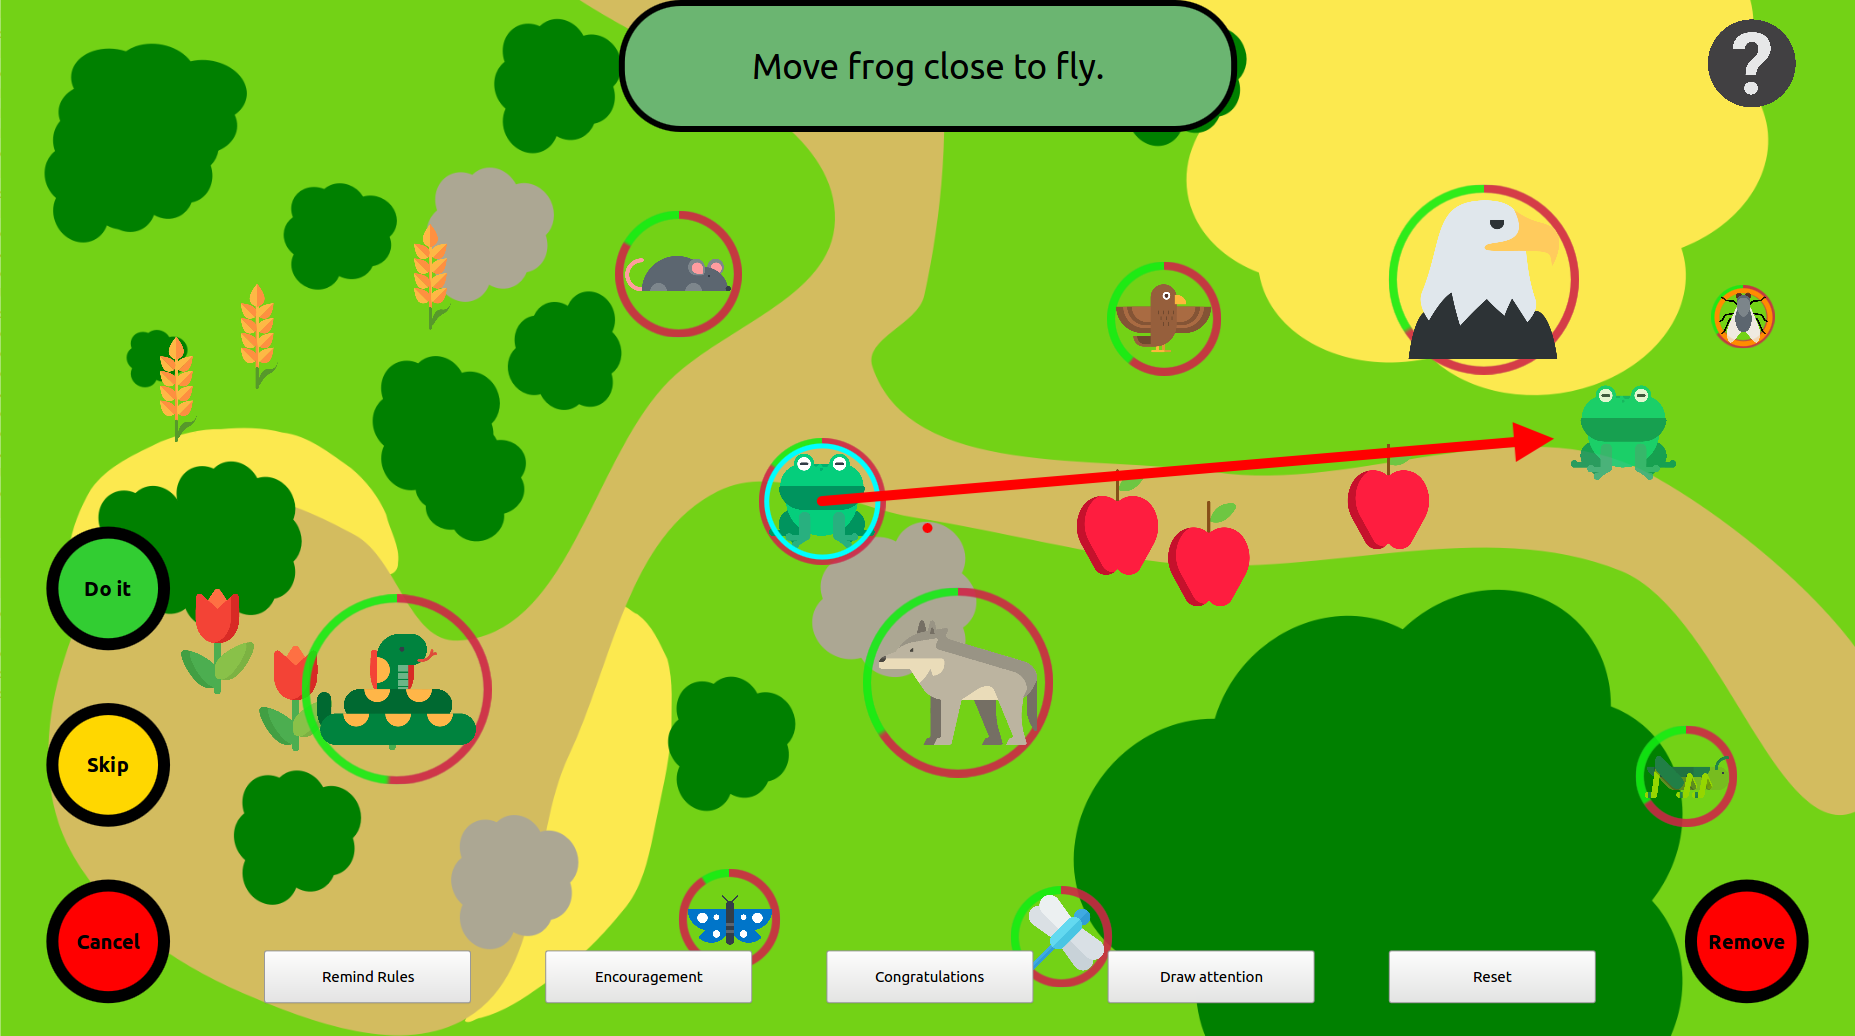
\includegraphics[width=1\textwidth]{gui.png}
	\caption{\gls{gui} used by the teacher to control the robot and respond to its suggestions. The game is in the same state as in Figure~\ref{fig:tutoring_game}, and the robot proposes to move the frog close to the fly (text bubble, arrow, moving the \textit{shadow} of the frog and highlight the frog and the fly).}
	\label{fig:tutoring_gui}
\end{figure}

Finally, the \gls{gui} also allows the teacher to respond to the robot's propositions. Following the proposition of an action, a bubble describing the action appears on top of the \gls{gui}, the corresponding items are highlighted and if the action is a motion, an arrow shows the proposed motion (Figure~\ref{fig:tutoring_gui}). The teacher can react to the proposed action by pressing the `Do it', `Skip', `Cancel' or `Remove' buttons or let the action be automatically executed after 2 seconds during which the bubble will become lighter to represent the passive acceptance of the action. The `Do it' button executes the action straight-away, the `Skip' button sends a `wait' action with a reward of 1 (indicating the robot should wait in this situation), the `Cancel' sends the proposed action with a reward of -1 and does not execute it (indicating that this action is not appropriate in this situation), and finally, the `Remove' button looks for the closest previous instance of the action in memory and removes it, preventing this instance to be used in later action selection. Actions executed by the robot are assigned a reward of 1. In each case, any item highlighted are associated to the action. 

\subsection{Teacher}
The teacher was a psychology PhD student from the University of Plymouth, with limited knowledge of computing and machine learning but with an understanding of human cognition. She had been instructed on how to control the robot using the GUI and the effect of each buttons. She was aware of the methodology used in the study but not the underlying implementation, she experimented controlling the robot in two interactions: one with the author interacting with the robot and one with a child before starting to supervise the robot for the supervised condition. No information about the learning algorithm or the representation of the state and no feedback about optimal way of interacting or on her action policy was provided before or during the supervision. As such, this study also demonstrates that novices and naive users are able to use this system to train personalised robot behaviour.

%the robot teacher represented typical target populations for robotic applications: non-experts in machine learning or computing but with relevant domain knowledge such as teachers, psychologists or more broadly, people from the general population.

% Figure~\ref{fig:tutoring_game} shows an example of the game screen. The child can move 10 animals across the game field and can have them interact with other animals or plants. Animals lose energy over time and by interacting with their food the can regain some. Animals that are eaten lose a chunk of their life. The goal for the children is to keep animals alive as long as possible by feeding them and they earn stars representing how healthy their animals have been during the round. The game stops when 3 or more animals run out of energy and each game round lasted 1.6 minutes in average.

\subsection{Conditions}
The study evaluated three conditions: the passive condition, supervised condition and autonomous condition. The conditions only impact the robot's behaviour during the game rounds. In each other part of the study, the robot's behaviour was identical between conditions.
%In all the conditions, the robot's behaviour during the introduction, tests, tutorial and conclusion was identical. The only change of behaviour happened during the games rounds. 
The study design was between participants, in all the game rounds, the robot was operated in the same way: either passive, supervised or autonomous.  %In the passive condition, the robot does not provide support during the game. In the supervised condition, the robot is controlled by a PhD student in psychology acting as the robot's teacher and demonstrating it how to interact. And in the autonomous condition, the robot simply applies the learned policy without supervision.

\subsubsection{Passive Condition}

The \textit{passive} condition served as a control condition. We decided to use a robot even in the control condition to prevent confounds related to the presence of a robot, such as novelty effect. The goal of the study was not to explore if a robot can be better than a human or than just the sandtray, but to study if by using \gls{sparc}, a human could teach the robot a behaviour which has a positive influence on the children in the game. Consequently, in this passive condition, the robot did not provide any advice or feedback to the children during the game rounds, it simply read the instructions and swayed. This condition was used as a baseline to compare to other ones.


%In the \textit{supervised} condition, the robot was remotely supervised by an operator using \gls{sparc}. Finally, in the \textit{autonomous} condition, the robot applied the learnt policy and provided feedback and guidance to the child without human supervision.


\subsubsection{Supervised Condition}

The \textit{supervised} condition was the one in which the robot `learned', where \gls{sparc} was used by a human to teach the robot an efficient action policy. As such, it was a dynamic condition where the robot interacted with the child and learned an action policy through the human's instructions, while the teacher herself was getting used to controlling the robot. In theory, throughout the different interactions with the children, the behaviour expressed by the robot should have been similar and constantly appropriate. In contrast, the teaching interaction between the teacher and the robot, should have evolved due to the learning component on the robot side. 

\subsubsection{Autonomous Condition}

The \textit{autonomous} condition was used to evaluate if the learned behaviour was efficient and if the robot could display a useful social action policy without being supervised. During this condition, the robot used the action policy taught in the supervised condition, but without the teacher in the loop. As such, this condition had to be run after the supervised one, when the teaching was over. %The role of this condition is to evaluate if the robot did learn a useful action policy, i.e. explore if after having been taught, the robot can have an autonomous behaviour having a positive impact on the child experience.

In the autonomous condition, the robot directly used the suggestions from the algorithm and executed them with a probabilistic delay between 0 and 1.5 seconds based on the teacher's delay in answering the robot's propositions. This delay aimed to give a pace and synchronisation of actions similar to the ones exhibited by the teacher when reacting to the robot's suggestion.

\subsection{Protocol}

%Parents completed a consent form and each child was proposed to withdraw if they appeared not interested to continue the study (children refusing to continue have been replaced to reach the same number in each category). 
At the start of the interaction, children were first introduced to the robot and were told they would play a game about food chains with the robot. Then, they completed a quick demographic questionnaire and a first pre-test to evaluate their baseline knowledge (cf. Figures~\ref{fig:tuto_pretest} to \ref{fig:tuto_test_results}). After this test, and before starting the teaching game, children had to complete a tutorial where they were introduced to the mechanics of the game: animals have life and have to eat to survive and children can move animals to make them interact with other animals or plants and replenish their energy (cf. Figures~\ref{fig:tuto_tuto_intro} and \ref{fig:tuto_tuto}). After this short tutorial, they completed two rounds of the game where the robot could provide feedback and advice depending on the condition they were in (cf. Figure~\ref{fig:tuto_game_intro} to \ref{fig:tuto_result_game}). Following these initial rounds of the game, children completed a mid-test before playing another two rounds of the game and completing a last post-test to conclude the study. Figure~\ref{fig:tuto_sequence} presents examples of screenshot of the Sandtray throughout the interaction.


\begin{figure}[ht]
	\centering
	\begin{subfigure}[b]{0.325\textwidth}
		\centering
		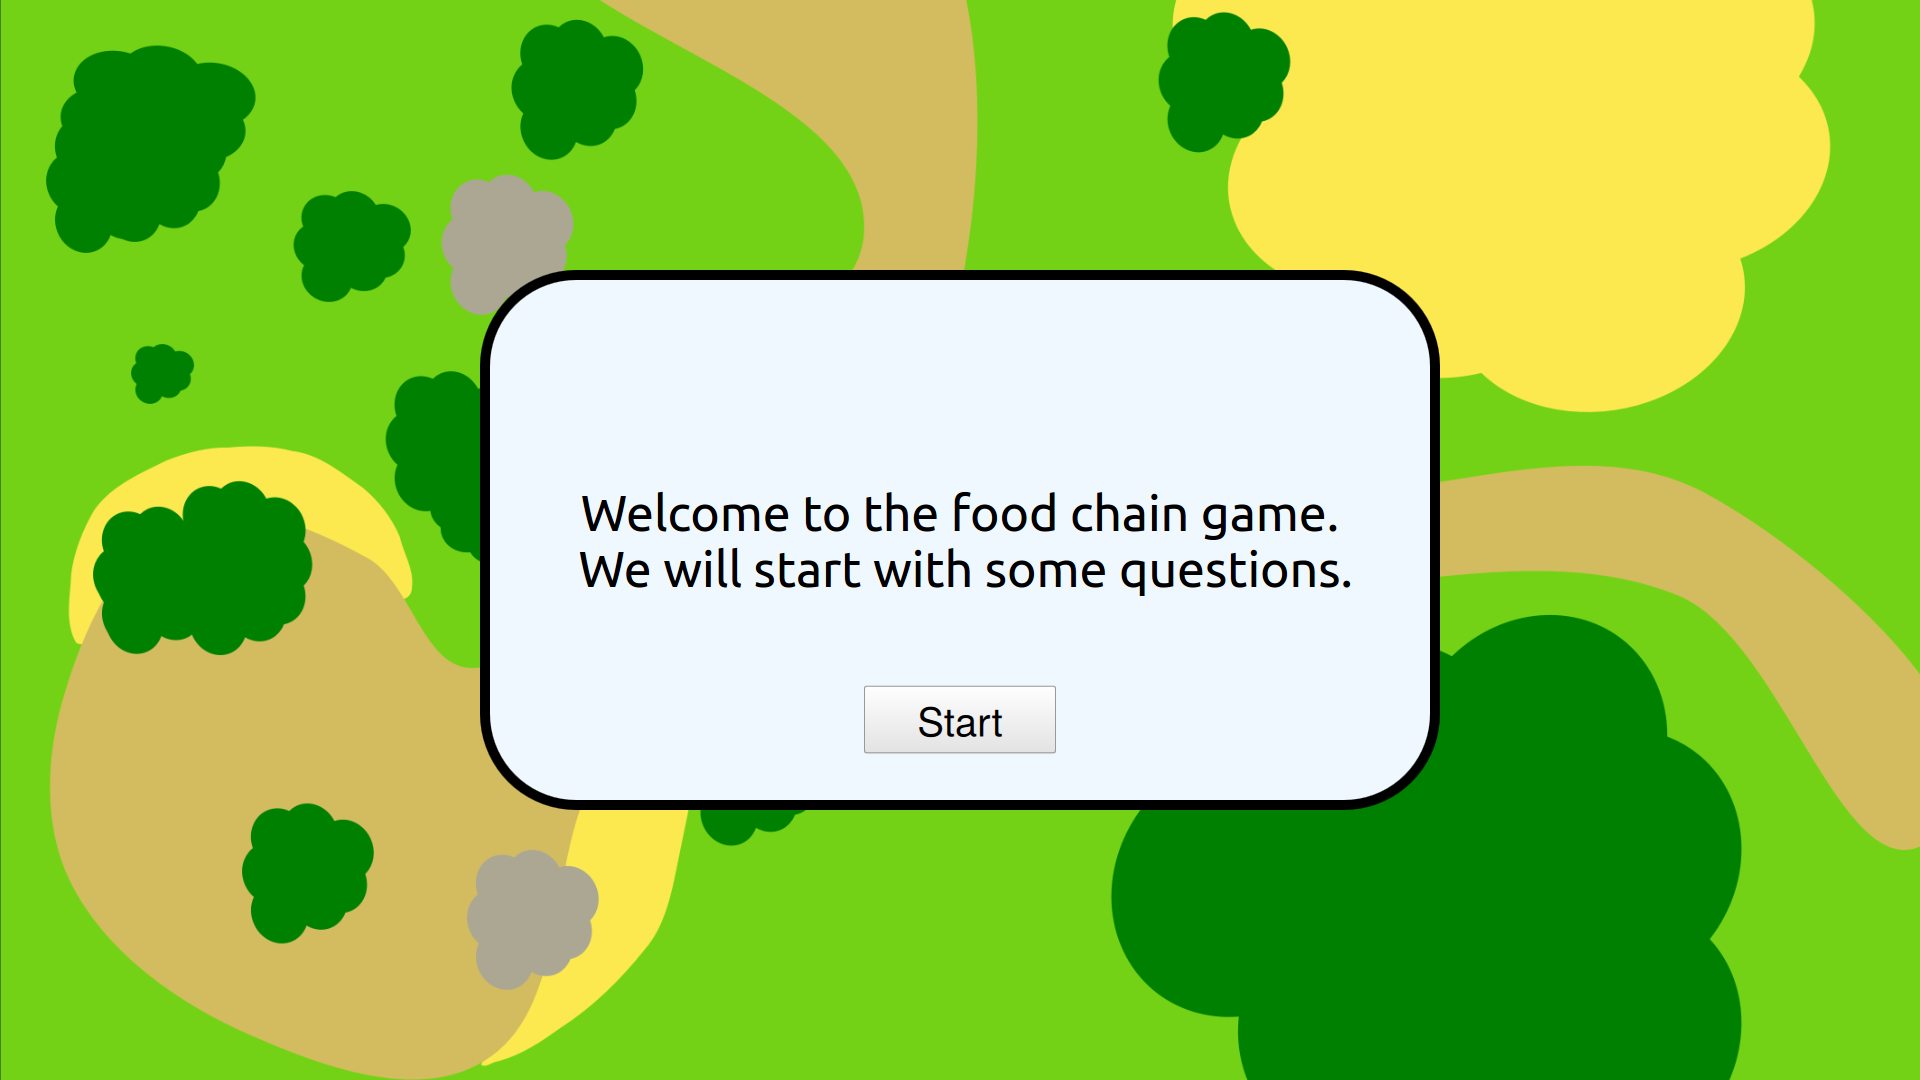
\includegraphics[width=\textwidth]{game_sequence/intro.png}
		\caption{Welcoming screen}
		\label{fig:tuto_welcome}
	\end{subfigure}
	\centering
	\begin{subfigure}[b]{0.325\textwidth}
		\centering
		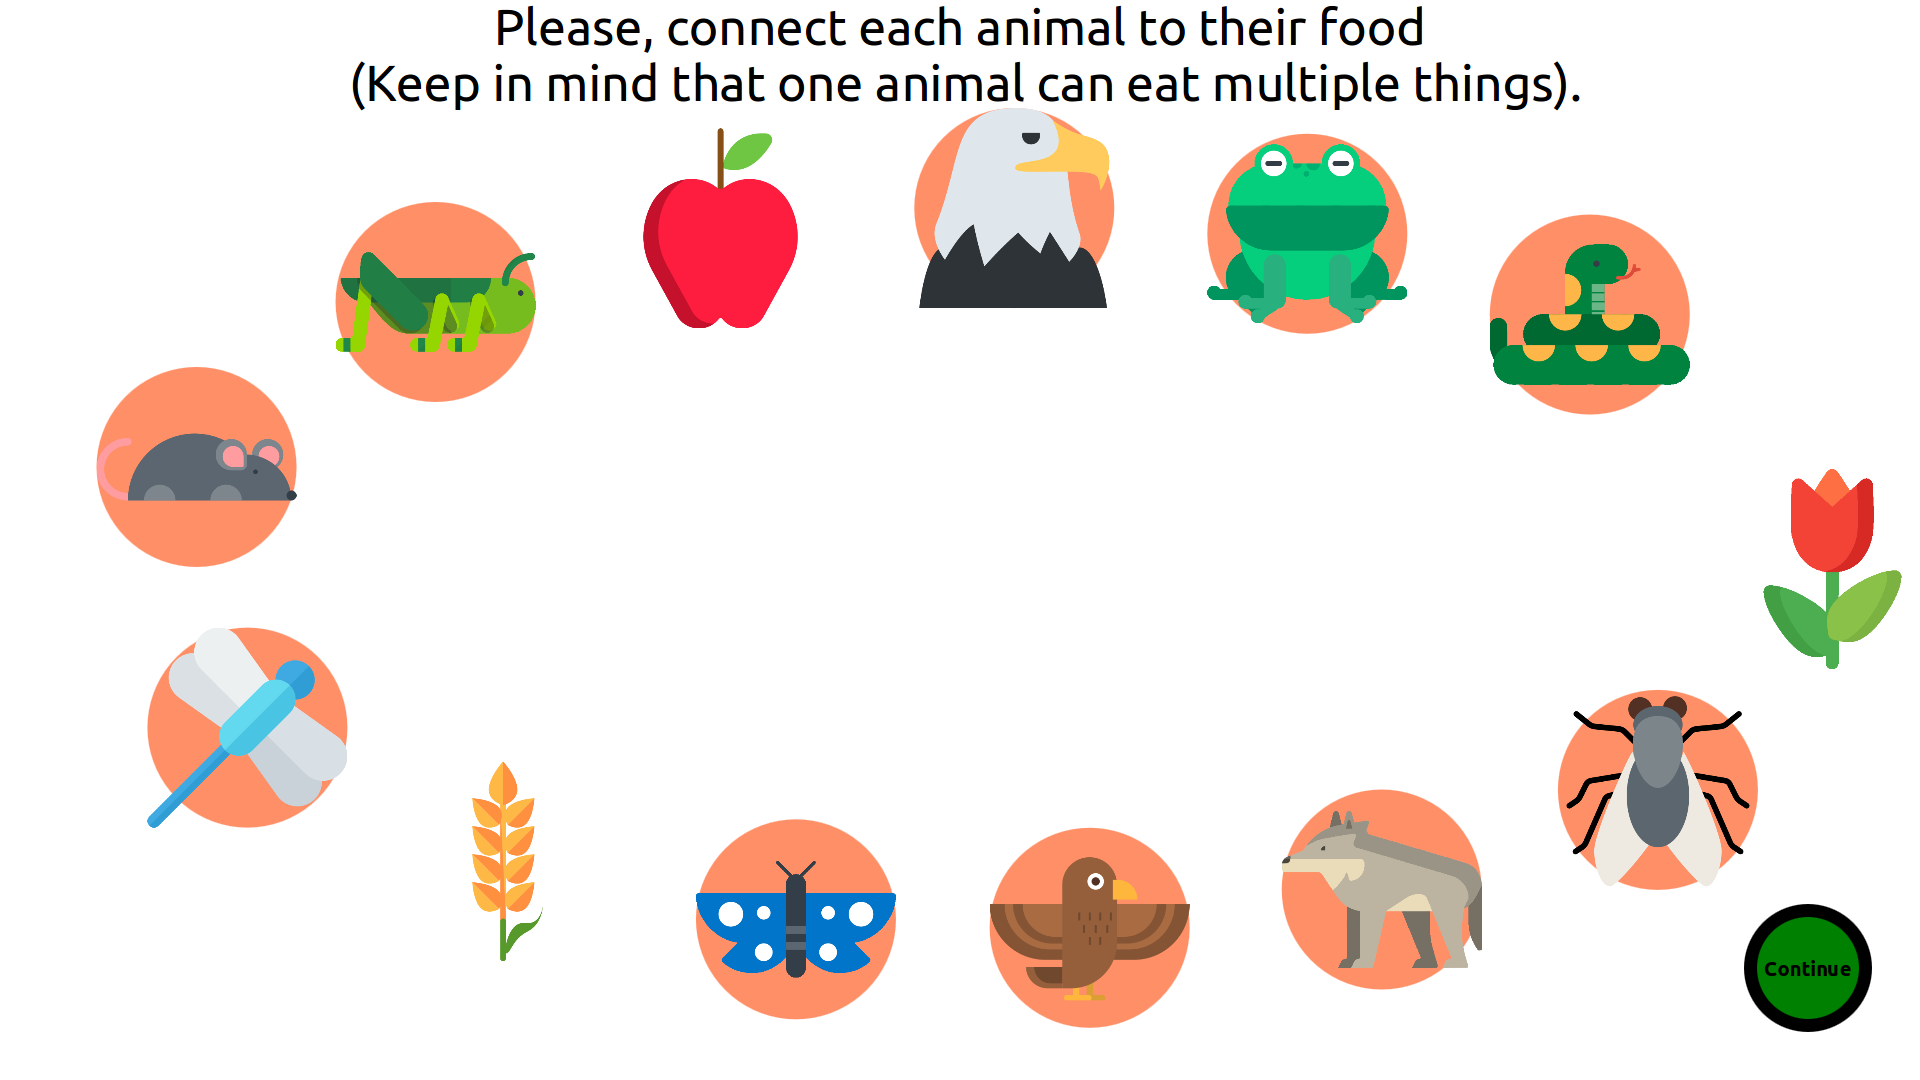
\includegraphics[width=\textwidth]{game_sequence/pretest.png}
		\caption{Test introduction}
		\label{fig:tuto_pretest}
	\end{subfigure}
	\centering
	\begin{subfigure}[b]{0.325\textwidth}
		\centering
		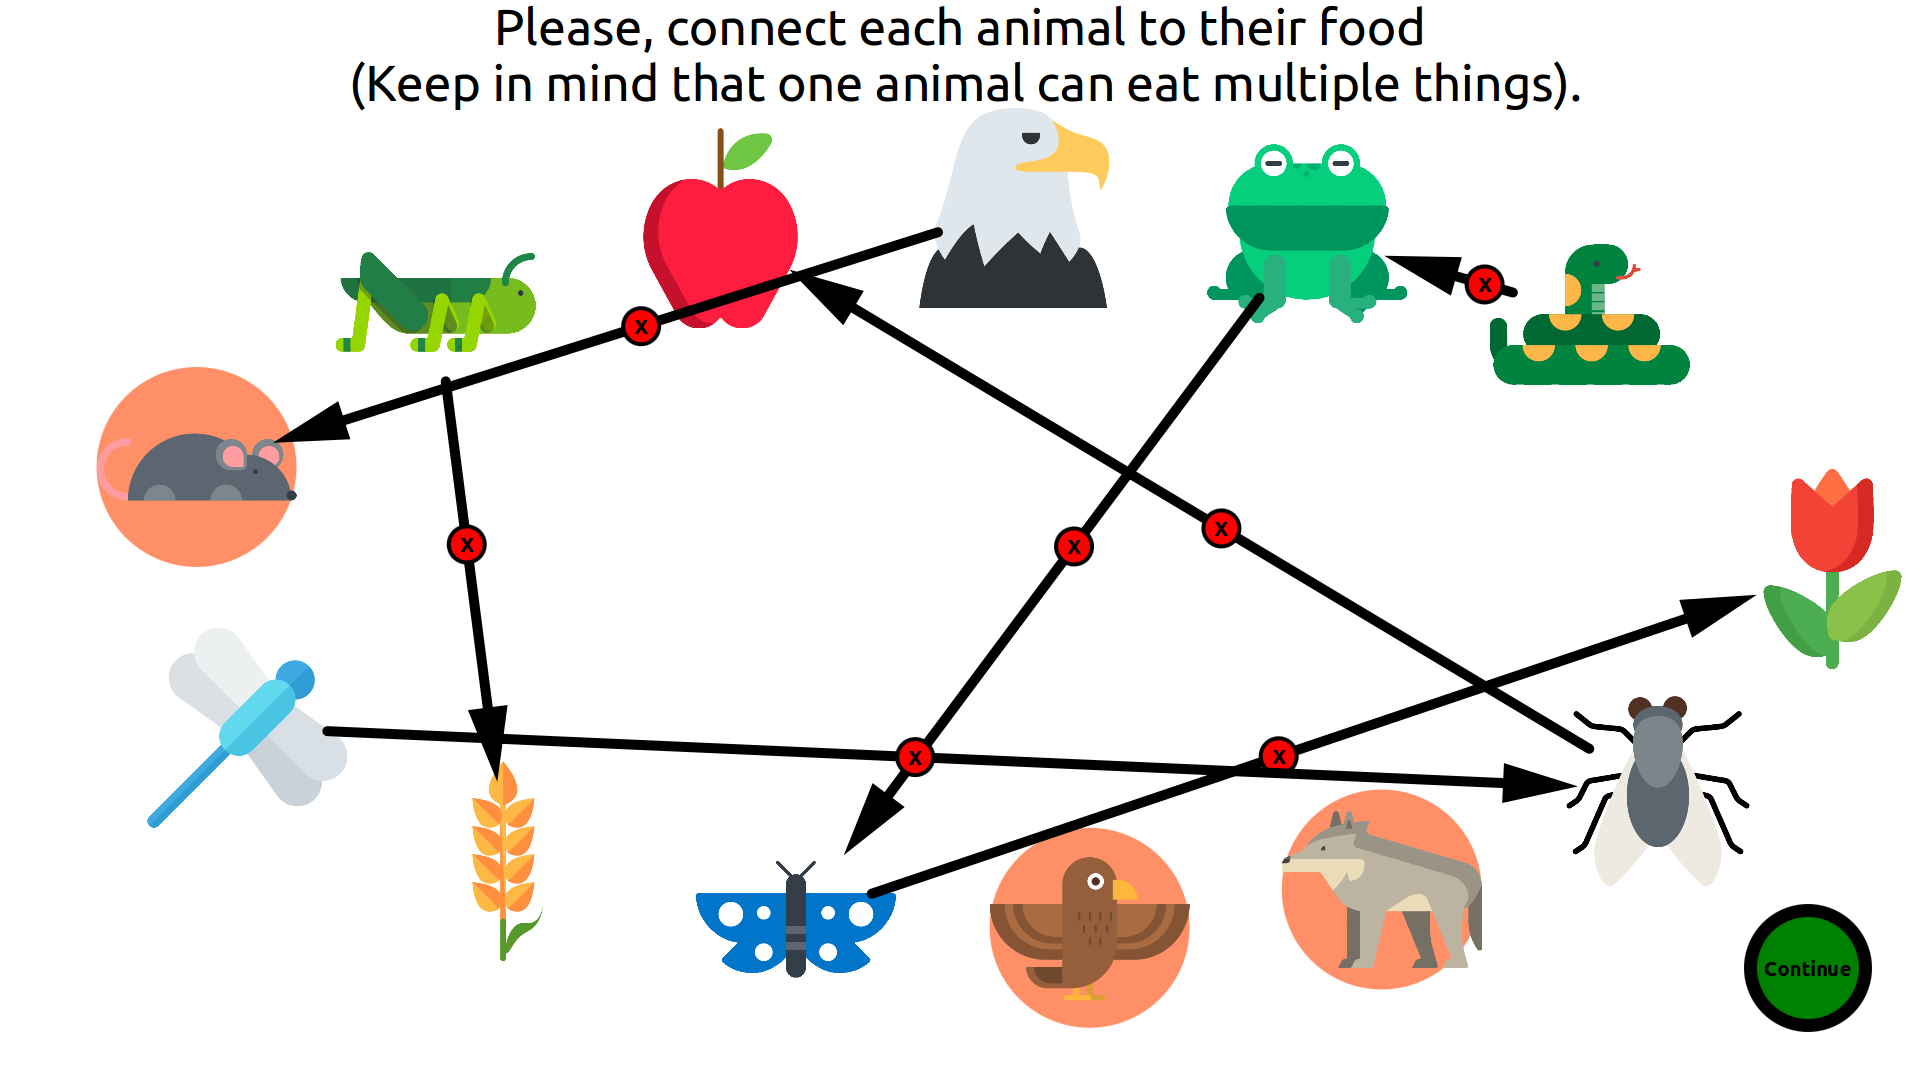
\includegraphics[width=\textwidth]{game_sequence/test_partial.png}
		\caption{Test partially completed}
		\label{fig:tuto_test_partial}
	\end{subfigure}
	\centering
	\begin{subfigure}[b]{0.325\textwidth}
		\centering
		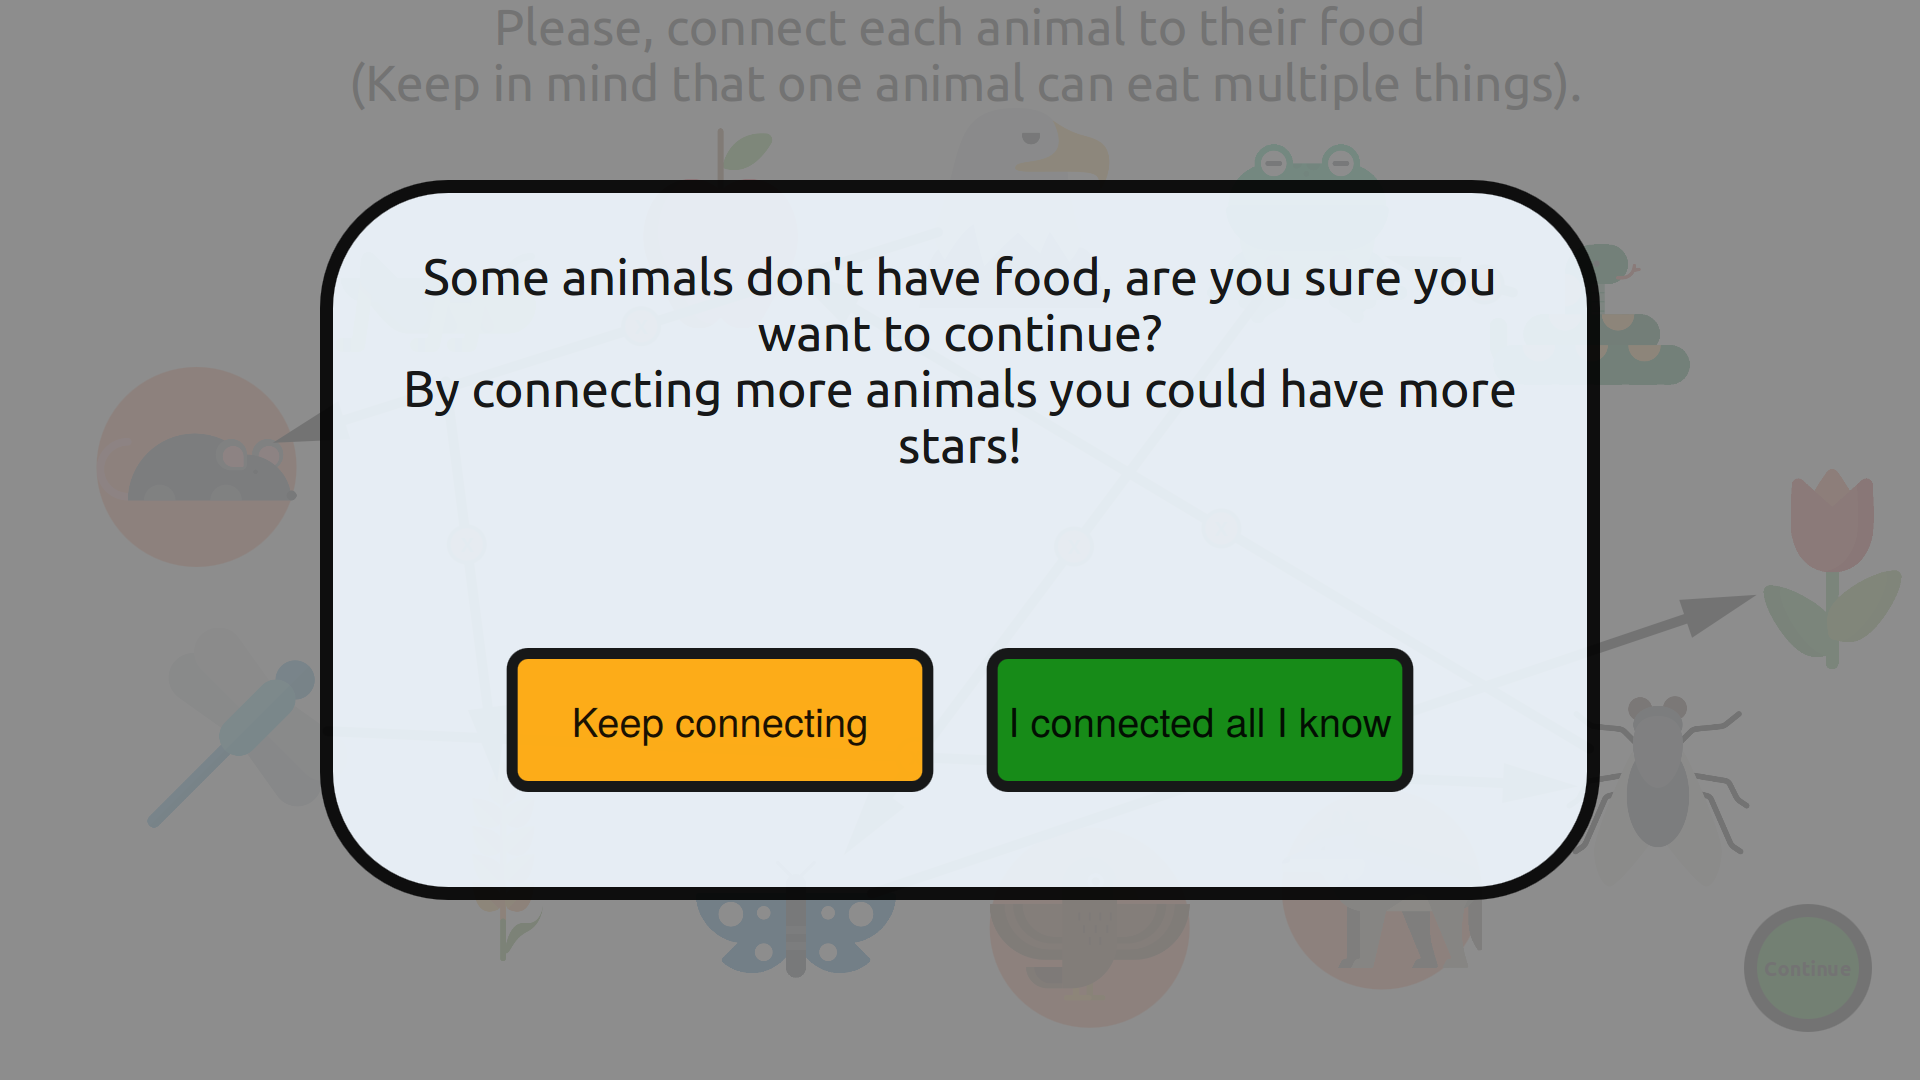
\includegraphics[width=\textwidth]{game_sequence/confirmation.png}
		\caption{Confirmation of test}
		\label{fig:tuto_test_confirmation}
	\end{subfigure}
	\centering
	\begin{subfigure}[b]{0.325\textwidth}
		\centering
		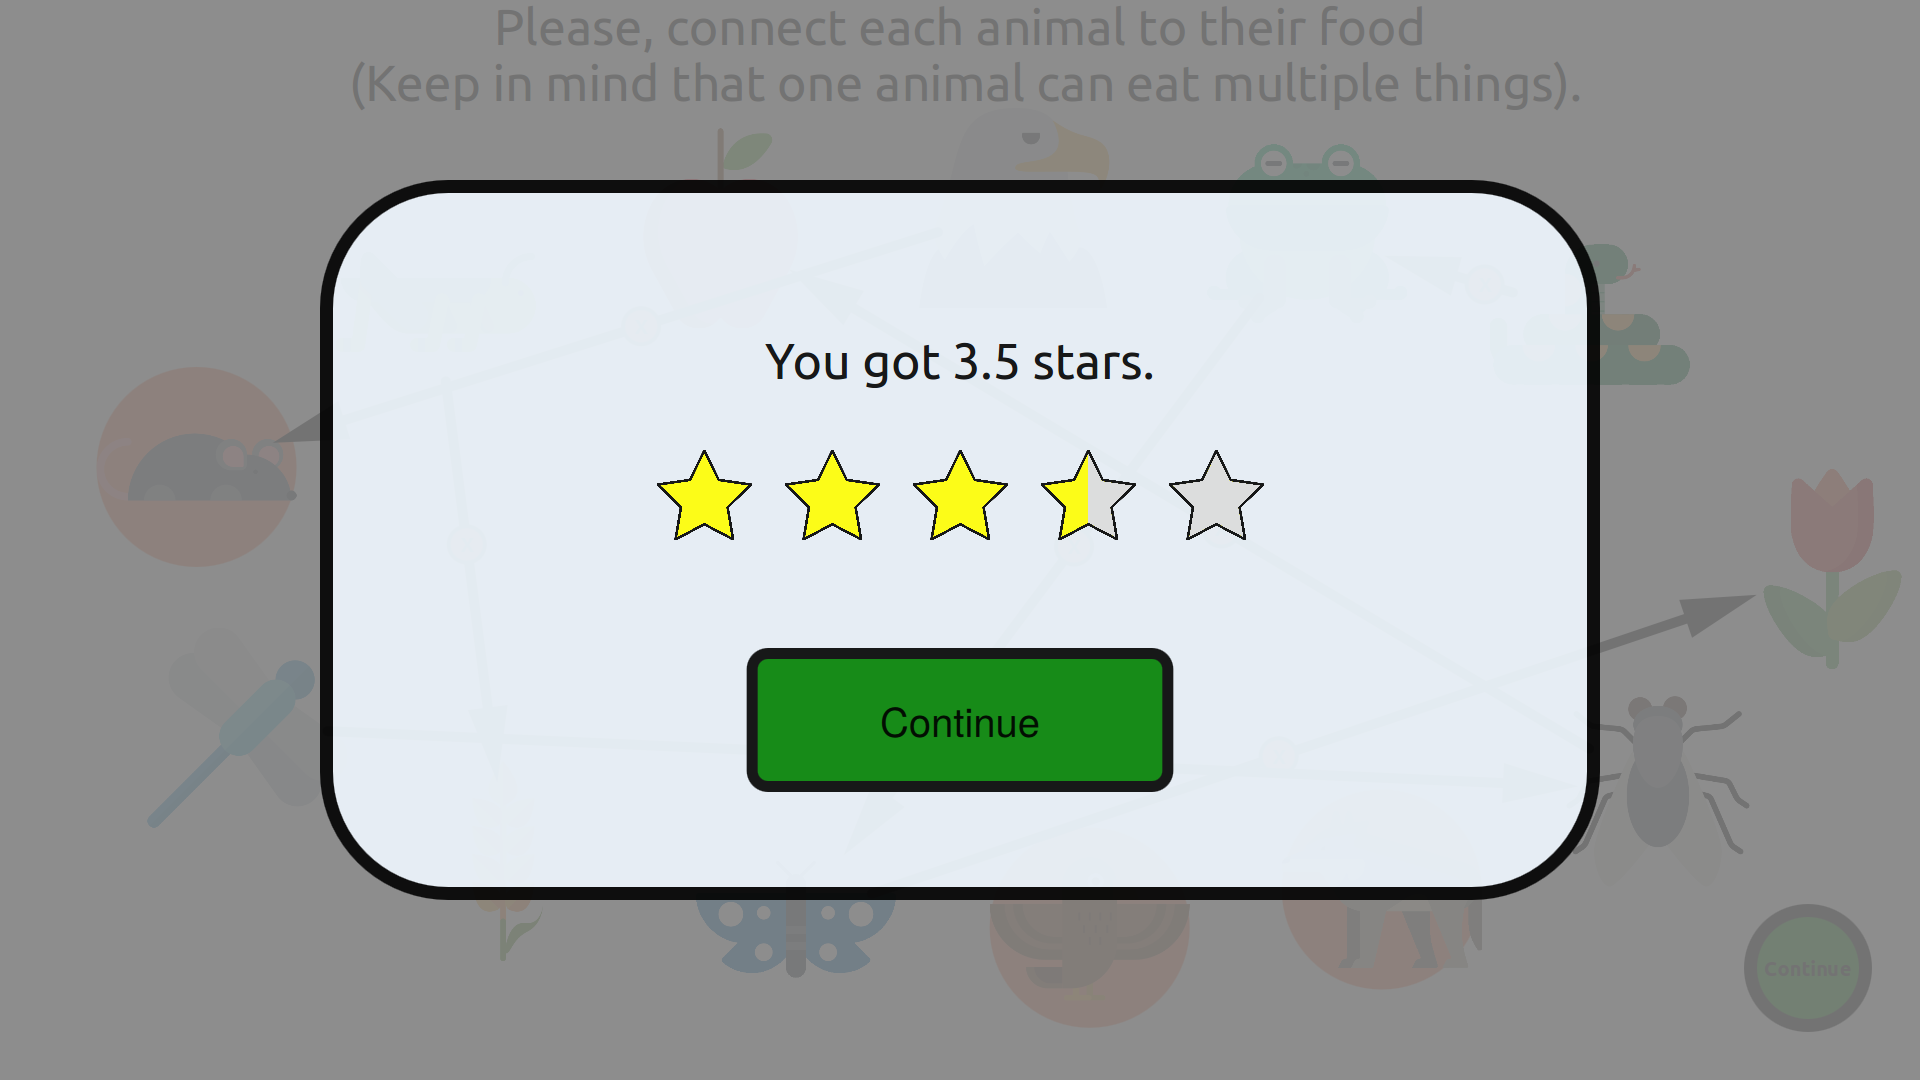
\includegraphics[width=\textwidth]{game_sequence/resulttest.png}
		\caption{Results of test}
		\label{fig:tuto_test_results}
	\end{subfigure}
	\centering
	\begin{subfigure}[b]{0.325\textwidth}
		\centering
		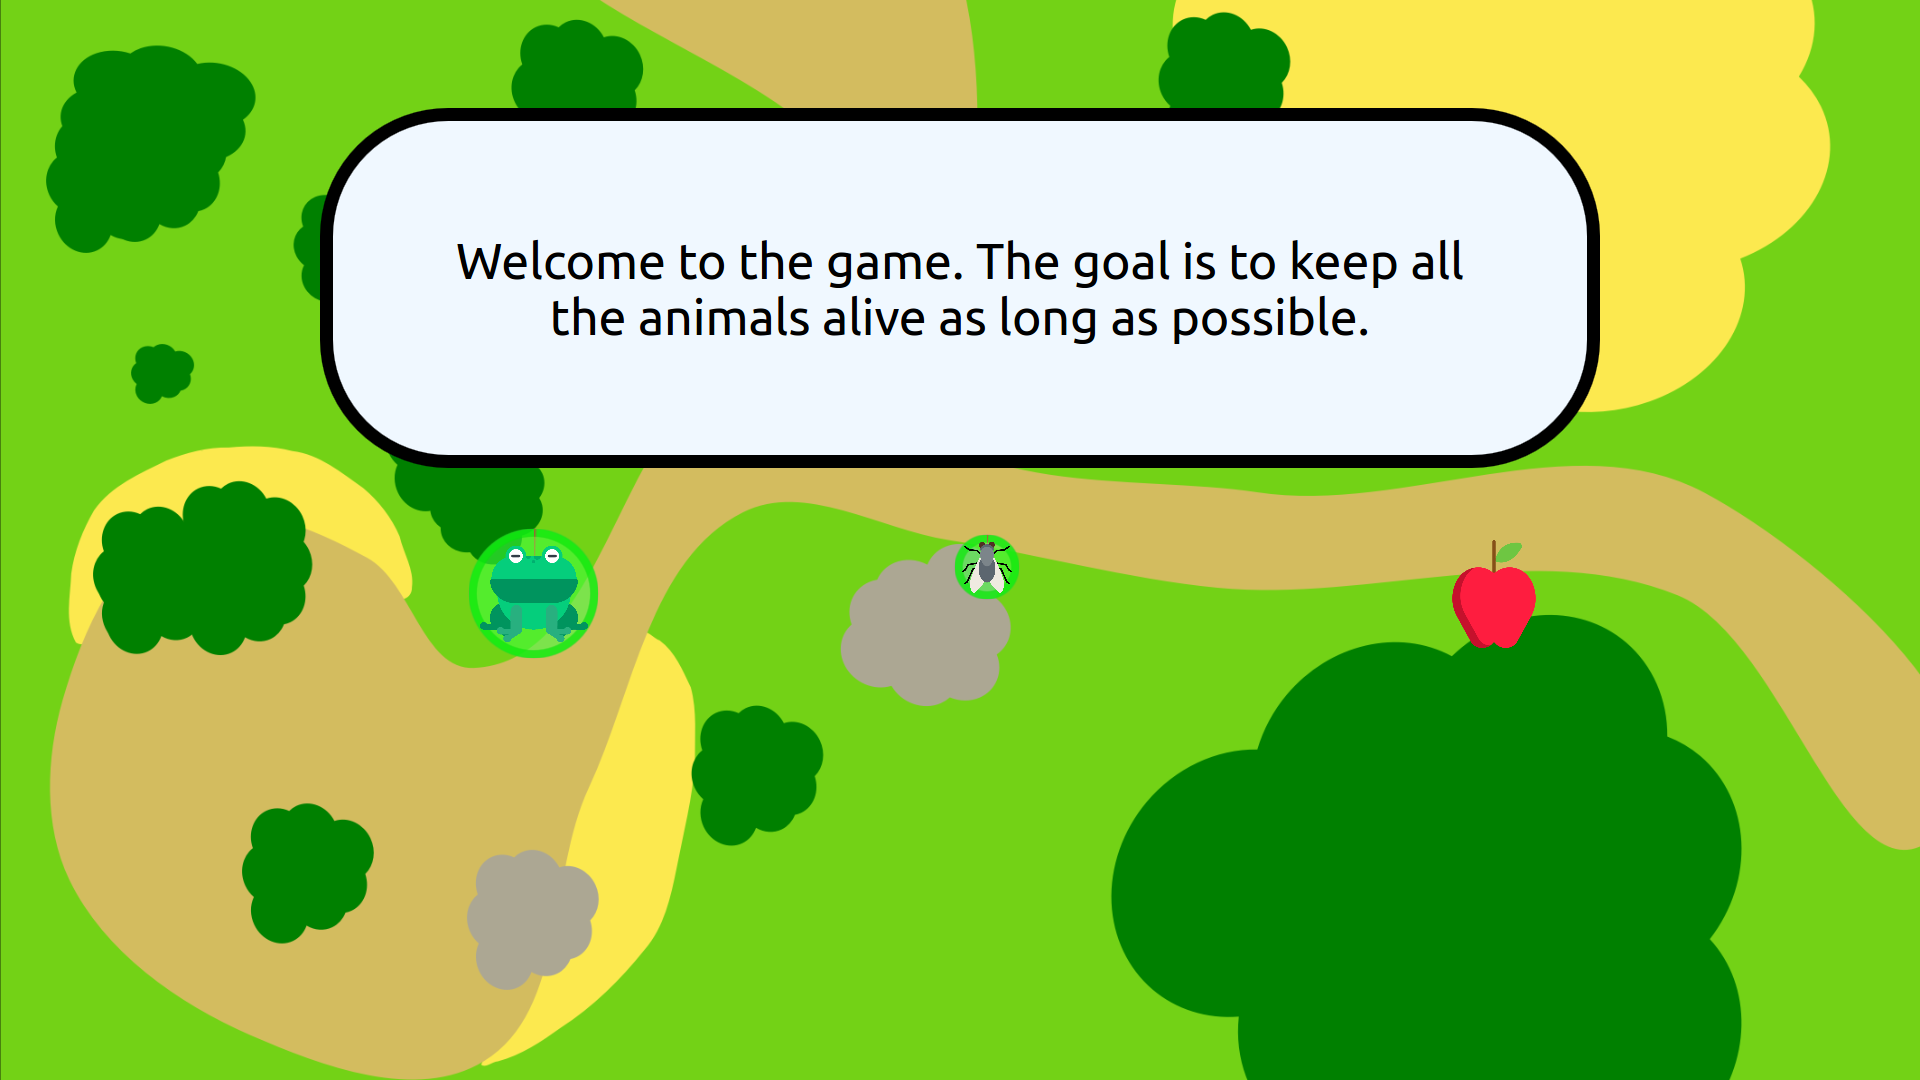
\includegraphics[width=\textwidth]{game_sequence/introtuto.png}
		\caption{Tutorial introduction}
		\label{fig:tuto_tuto_intro}
	\end{subfigure}
	\centering
	\begin{subfigure}[b]{0.325\textwidth}
		\centering
		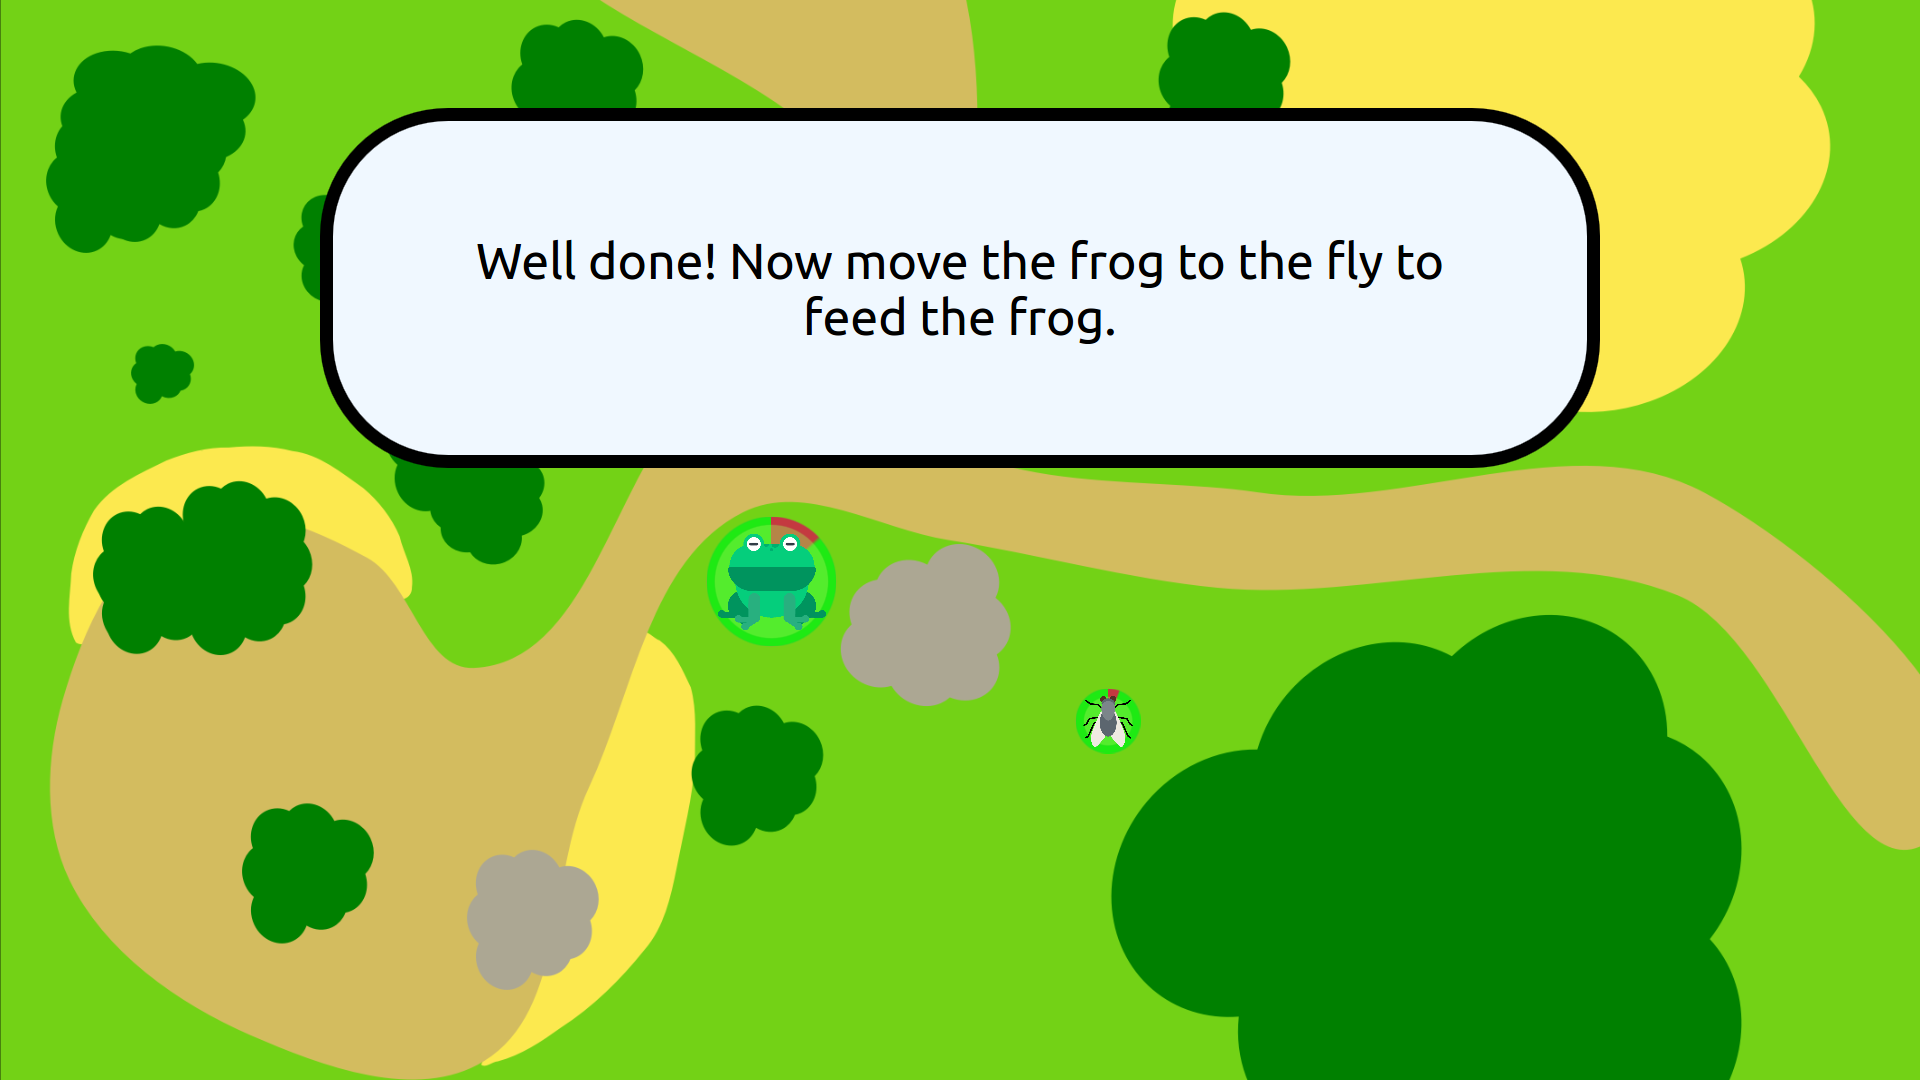
\includegraphics[width=\textwidth]{game_sequence/tutorial.png}
		\caption{Tutorial in progress}
		\label{fig:tuto_tuto}
	\end{subfigure}	
	\begin{subfigure}[b]{0.325\textwidth}
		\centering
		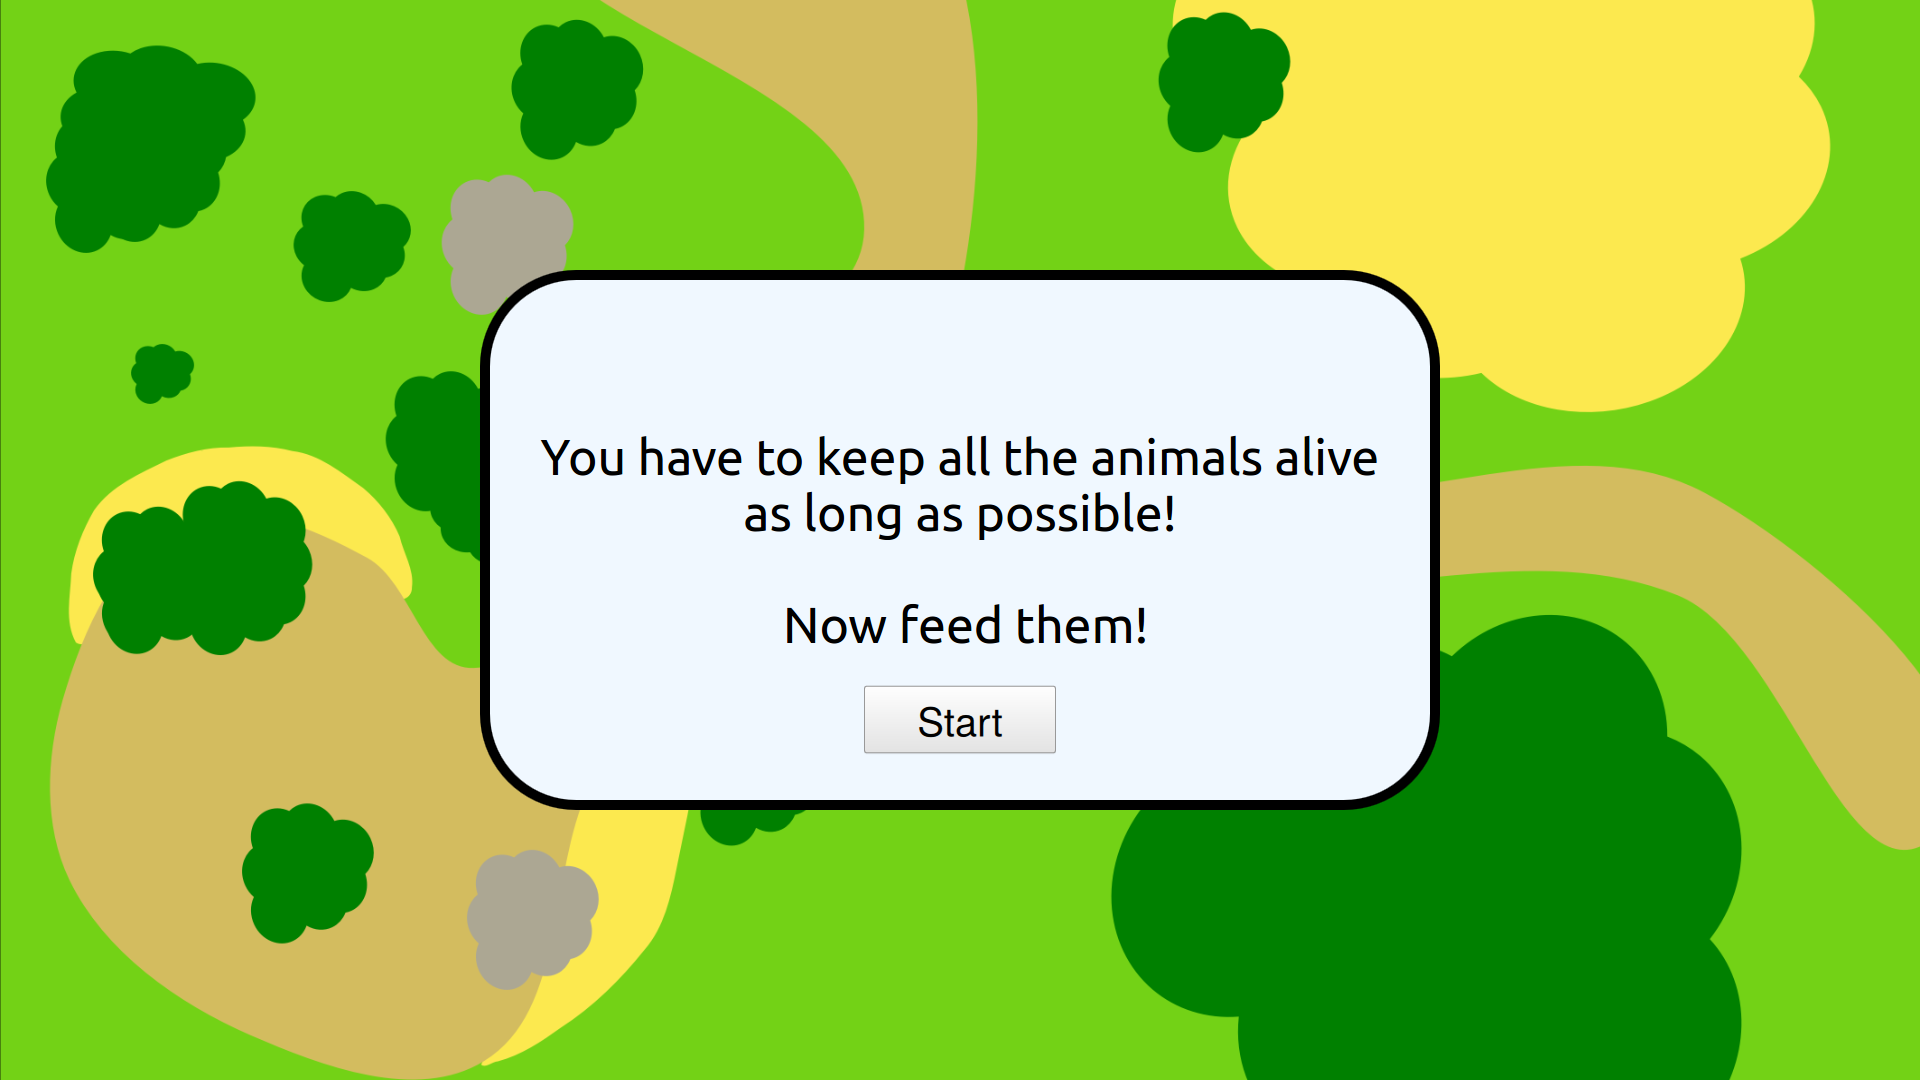
\includegraphics[width=\textwidth]{game_sequence/introgame.png}
		\caption{Game introduction}
		\label{fig:tuto_game_intro}
	\end{subfigure}
	\centering
	\begin{subfigure}[b]{0.325\textwidth}
		\centering
		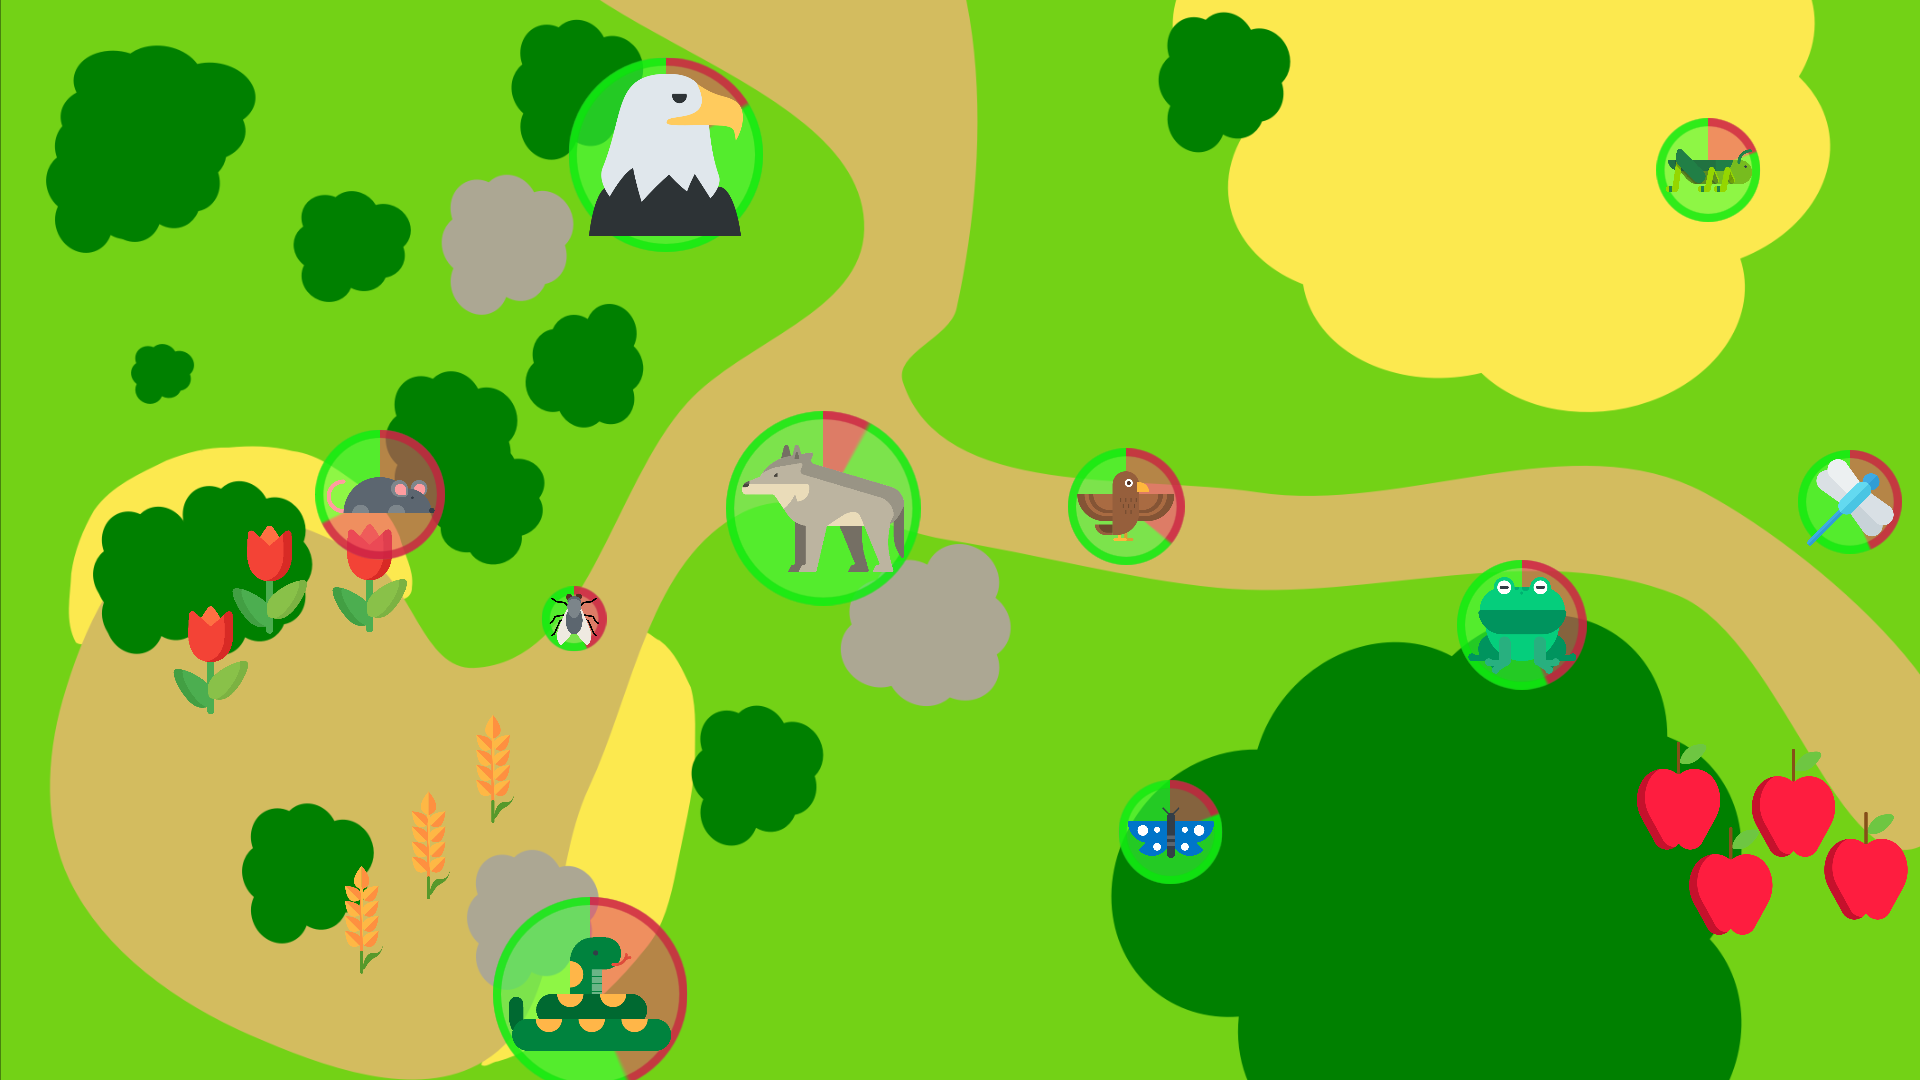
\includegraphics[width=\textwidth]{game_sequence/game1.png}
		\caption{Game in progress}
		\label{fig:tuto_game}
	\end{subfigure}	
		\centering
		\begin{subfigure}[b]{0.325\textwidth}
		\centering
		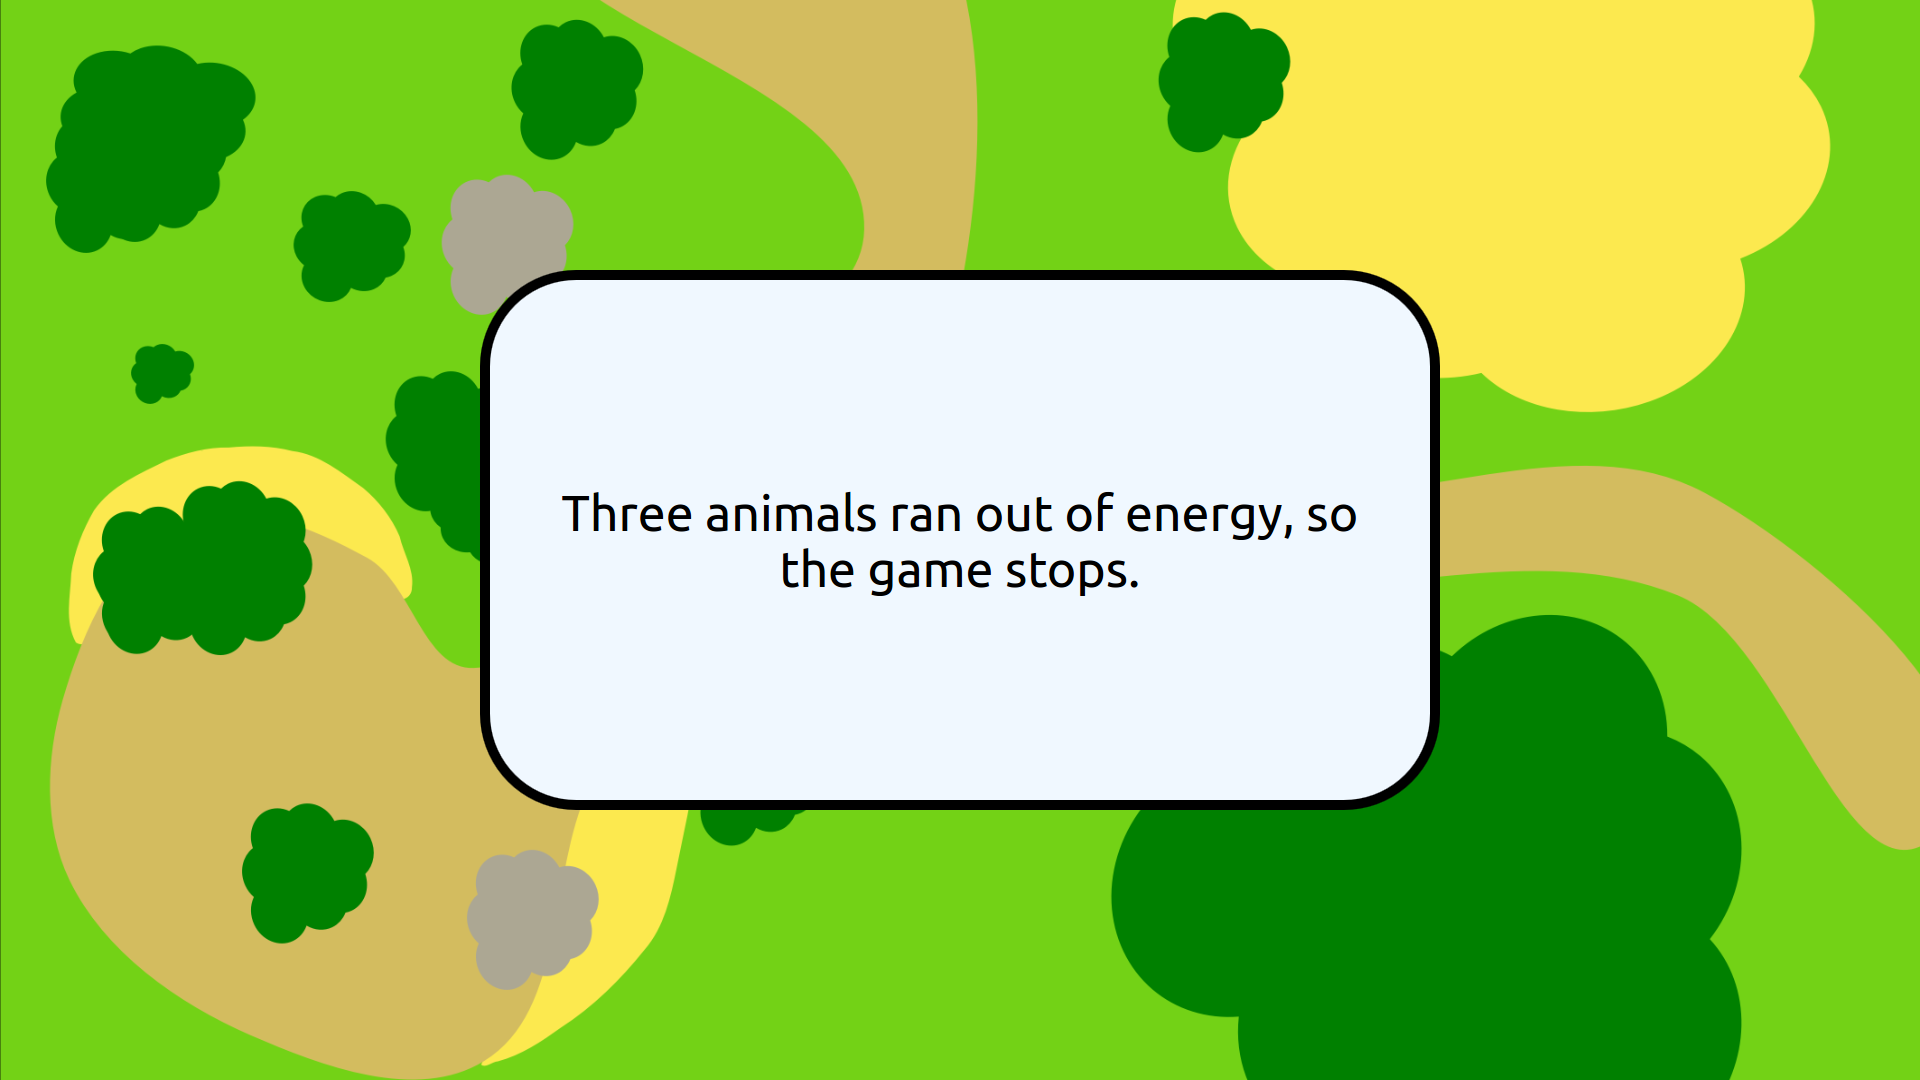
\includegraphics[width=\textwidth]{game_sequence/endgame.png}
		\caption{End of a game round}
		\label{fig:tuto_endgame}
	\end{subfigure}	
	\centering
	\begin{subfigure}[b]{0.325\textwidth}
		\centering
		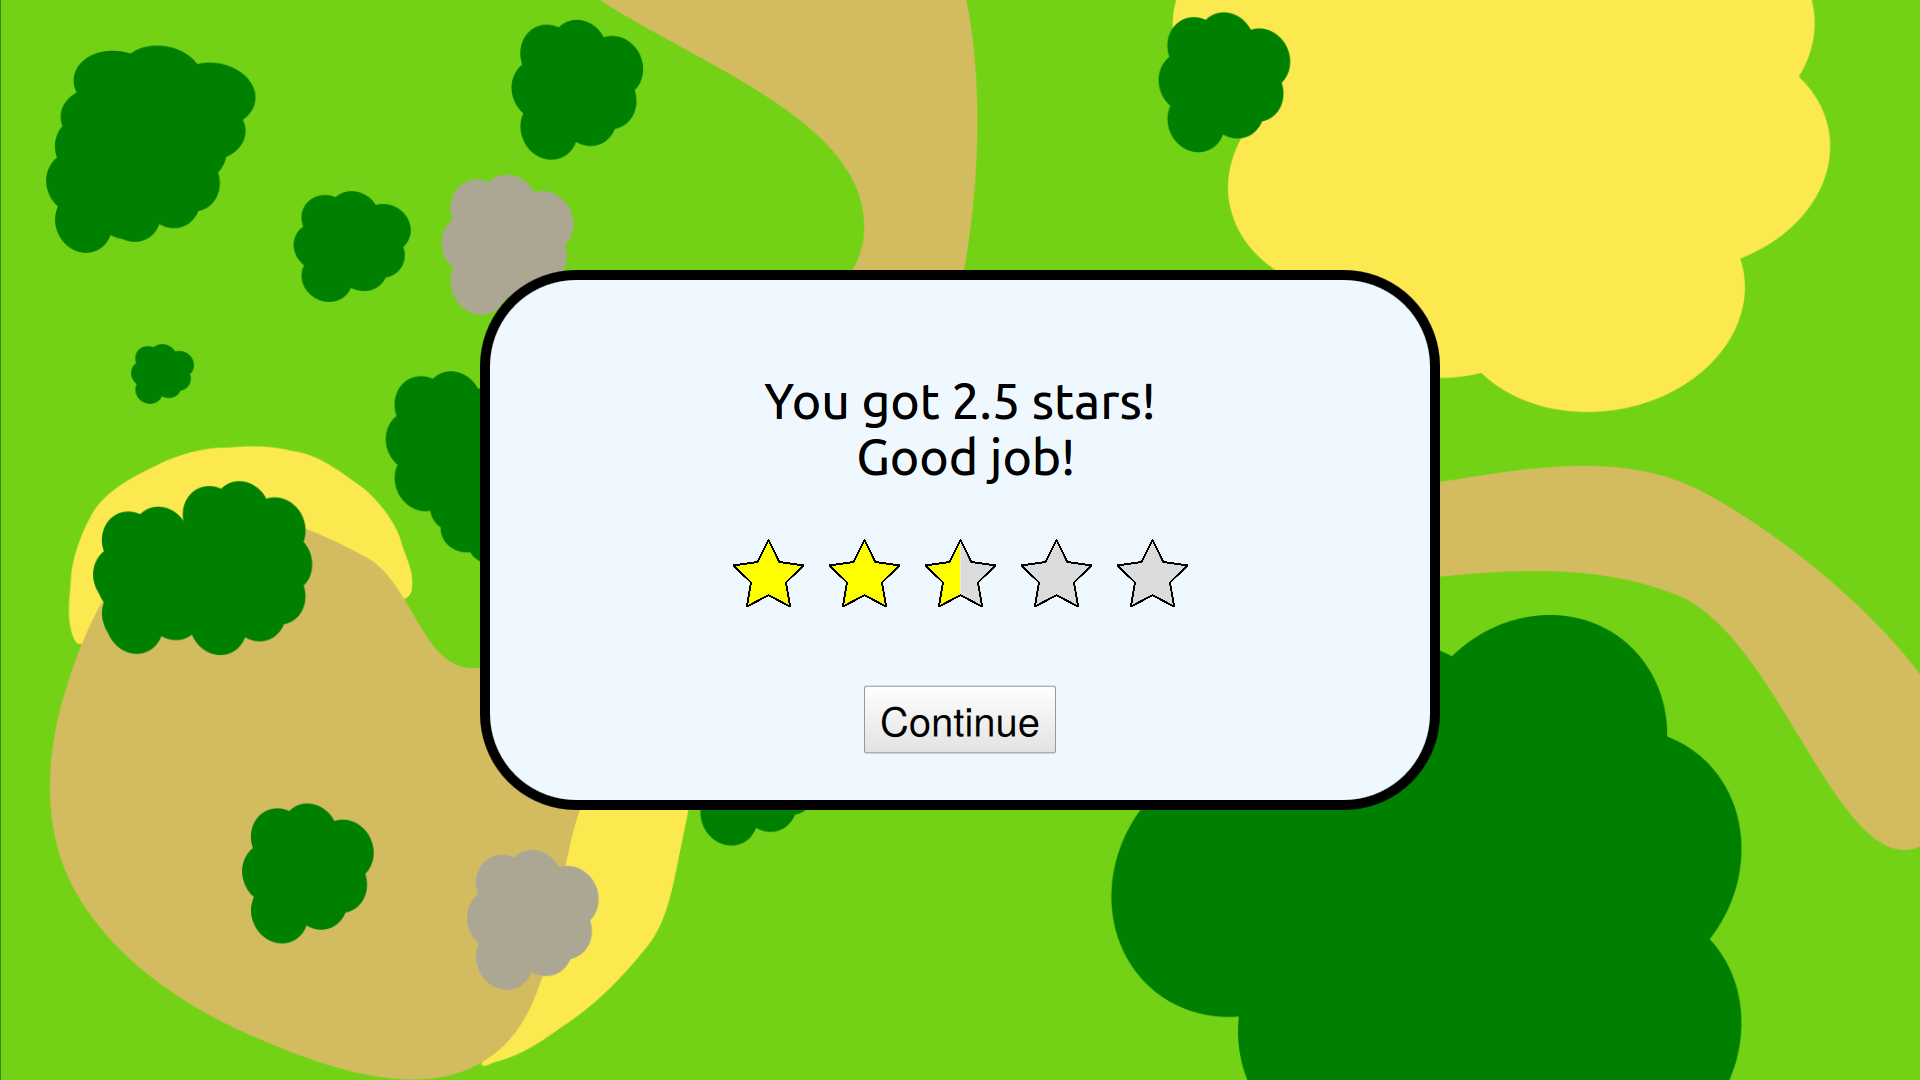
\includegraphics[width=\textwidth]{game_sequence/resultgame.png}
		\caption{Results of a game round}
		\label{fig:tuto_result_game}
	\end{subfigure}	
	\centering
	\begin{subfigure}[b]{0.325\textwidth}
		\centering
		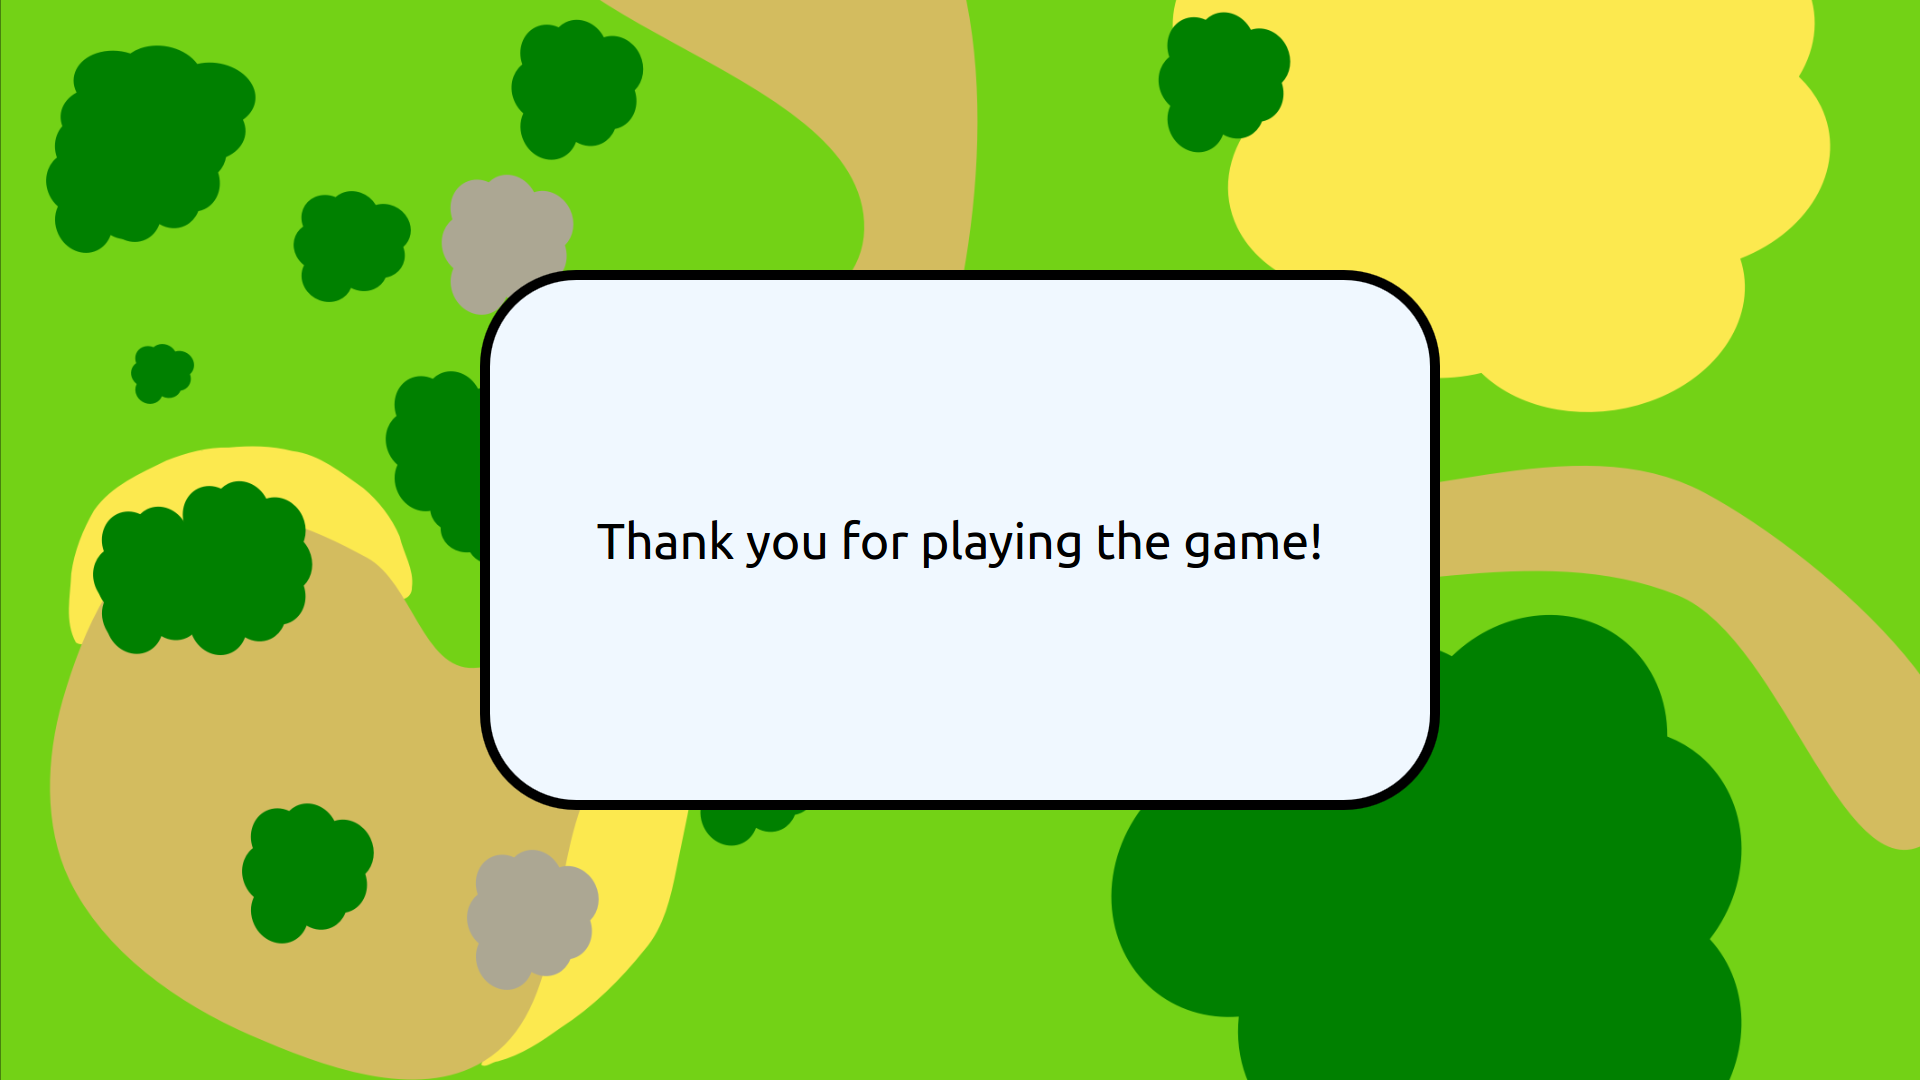
\includegraphics[width=\textwidth]{game_sequence/end.png}
		\caption{End of the interaction}
		\label{fig:tuto_end}
	\end{subfigure}	
	
	\caption{Presentation of different steps in the interaction. It should be noted that steps (b) to (e) correspond to one test and (h) to (k) to one game round. As such, a full interaction would see a first pretest (steps b to e), followed the tutorial (steps f and g), two game rounds (2 repetitions of steps h to k), a second test, two other game rounds and a last posttest before ending the interaction with step (l).}
	\label{fig:tuto_sequence}
\end{figure}

%\begin{figure}[h]
%	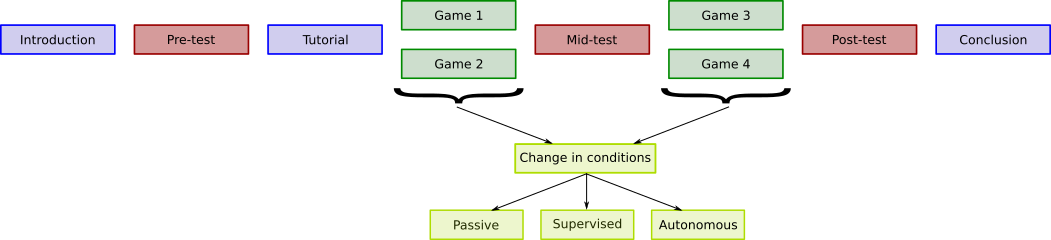
\includegraphics[width=.9\linewidth]{graph.png}
%	\centering
%	\caption{Methodology used for the study.}
%	\label{fig:method}
%\end{figure}

\subsection{Metrics}

%Redundant with hypothese?
%This study aimed mostly at evaluating if \gls{sparc} allows a human non-expert in computing to teach a robot from \textit{in situ} supervision. 
%This teaching capability is divided into three parts: 
%\begin{itemize}
%	\item How similar the teacher's and autonomous robot's policies are? 
%	\item What are the impacts of the active robot on the child behaviour? \\(And what are the differences between the autonomous and supervised robots?)
%	\item How the online learning component changed the interaction between the robot and the teacher?
%\end{itemize}

To address the hypotheses presented in Section~\ref{sec:tutoring_scope}, we collected multiple metrics on both interactions (teacher-robot and robot-child). First, we recorded the actions executed by the robot in the supervised and autonomous conditions to characterise the two action policies. Additionally, two groups of metrics have been collected to evaluate the application interaction: the learning metrics (corresponding to the child's performance during the test) and the game metrics (corresponding to the child's behaviour within the game). And finally, in the supervised condition, we recorded the origin of the action executed by the robot (teacher vs algorithm) and the outcome of the proposed actions (executed vs refused).

\subsubsection{Policy Characterisation}

During the game, the robot had access to 655 actions, which can be divided into seven categories: drawing attention, moving close, moving away, moving to, congratulation, encouragement and reminding rules. Due to this high number of actions, the largeness of the state space (210 dimension) and the complex interdependence between actions and states, totally defining a policy is impossible. Consequently, we decided to use the number of actions executed for each category per child to characterise the policy executed by the robot in the active conditions (supervised and autonomous). While not perfectly representing the action policy of each condition (e.g. the timing of actions is missing), this metric offers a proxy to compare these policies. 

\subsubsection{Learning Evaluation}
The learning was evaluated through an open graph where children had to connect animals to their food. Figure~\ref{fig:test} shows two examples of the test, with or without all the correct connections. Children were instructed to connect as many animals as possible. During the pre-test, the experimenter demonstrated how to connect animals by drawing an arrow from the frog to the fly, and then removing the arrow by pressing the X button in the middle of the arrow. When children thought they were done, they could press the `Continue' button, showing a screen asking confirmation to quit the test or allowing children to keep connecting animals. Additionally, the robot informed the child if not all the animals were connected to a food or that animals could eat many types of food if no more than one animal was connected to two items. 

\begin{figure*}[ht]
	\centering
	\begin{subfigure}[t]{0.5\textwidth}
		\centering
		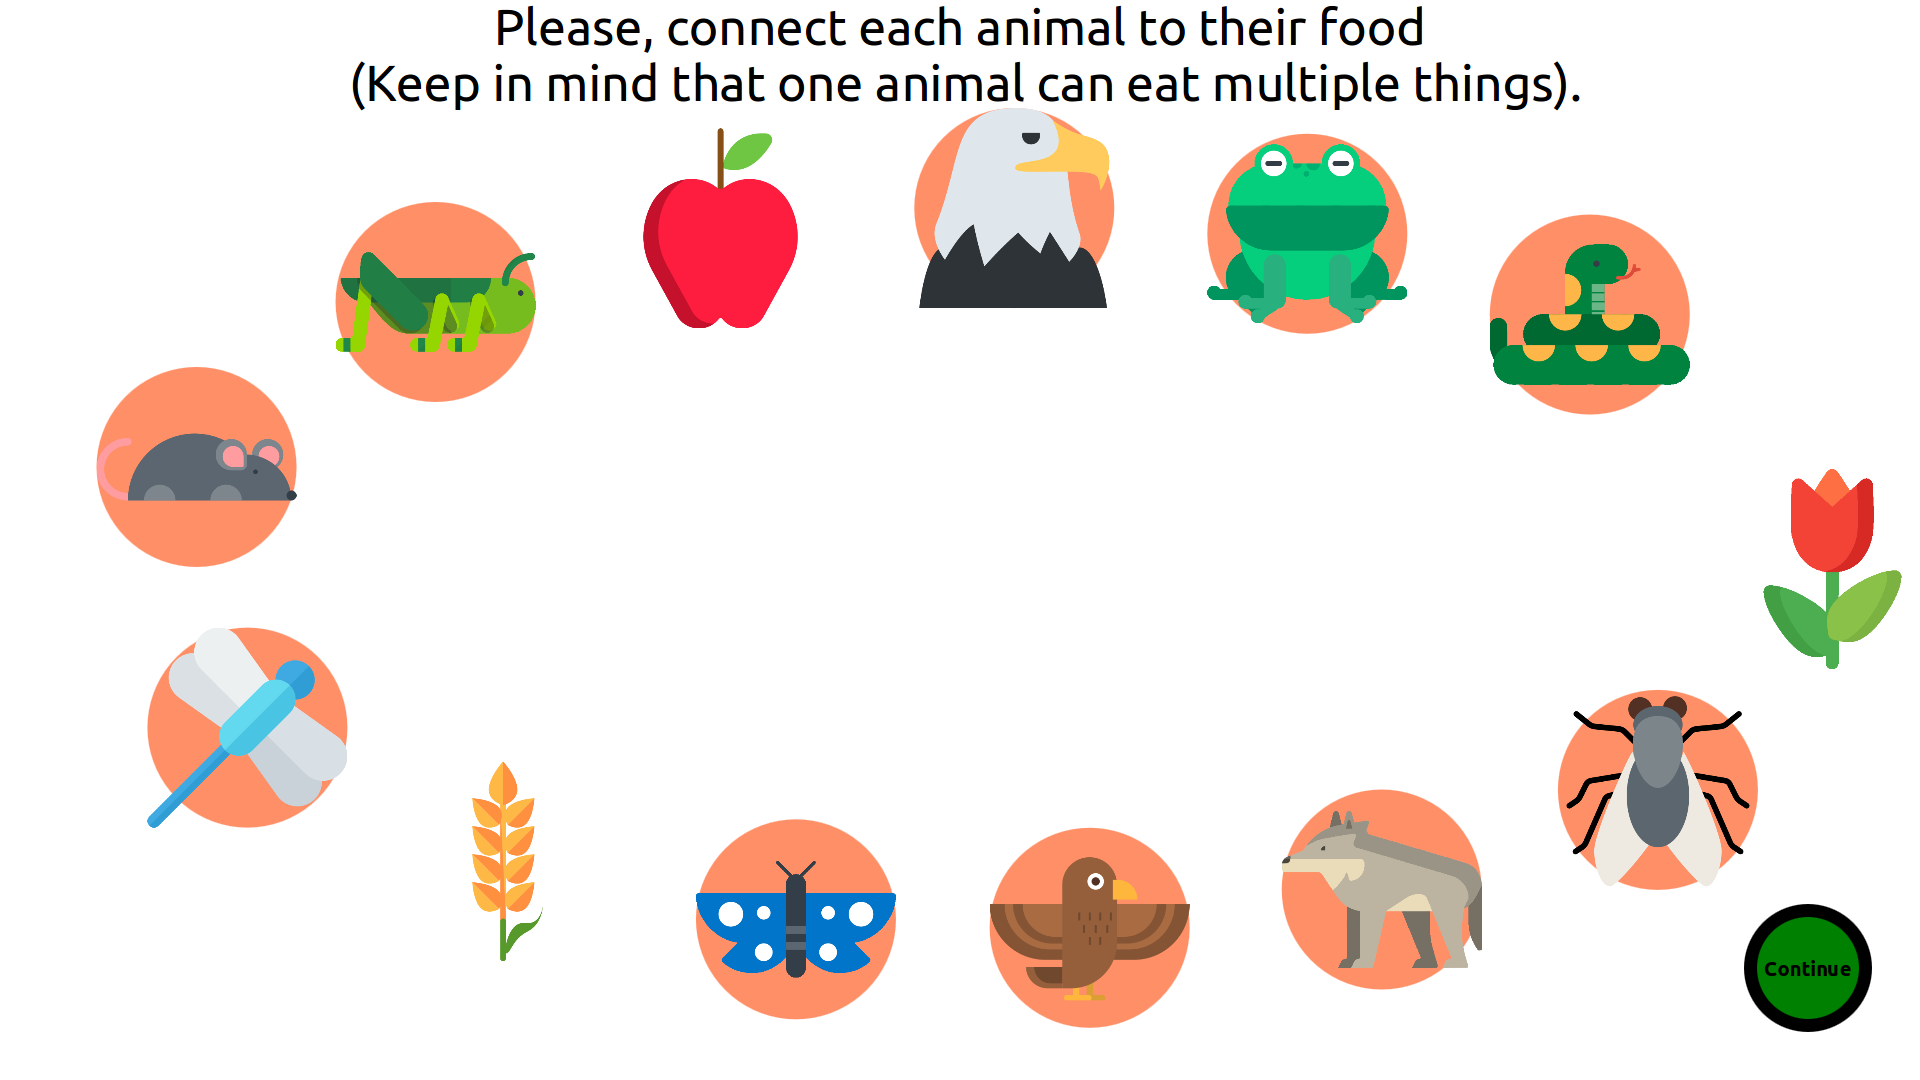
\includegraphics[width=0.95\textwidth]{empty_graph.png}
		\captionsetup{width=.95\linewidth}
		\caption{Empty screen that children face at each test. Red dots behind animals indicate that they are not connected to any food.}
	\end{subfigure}%
	~ 
	\begin{subfigure}[t]{0.5\textwidth}
		\centering
		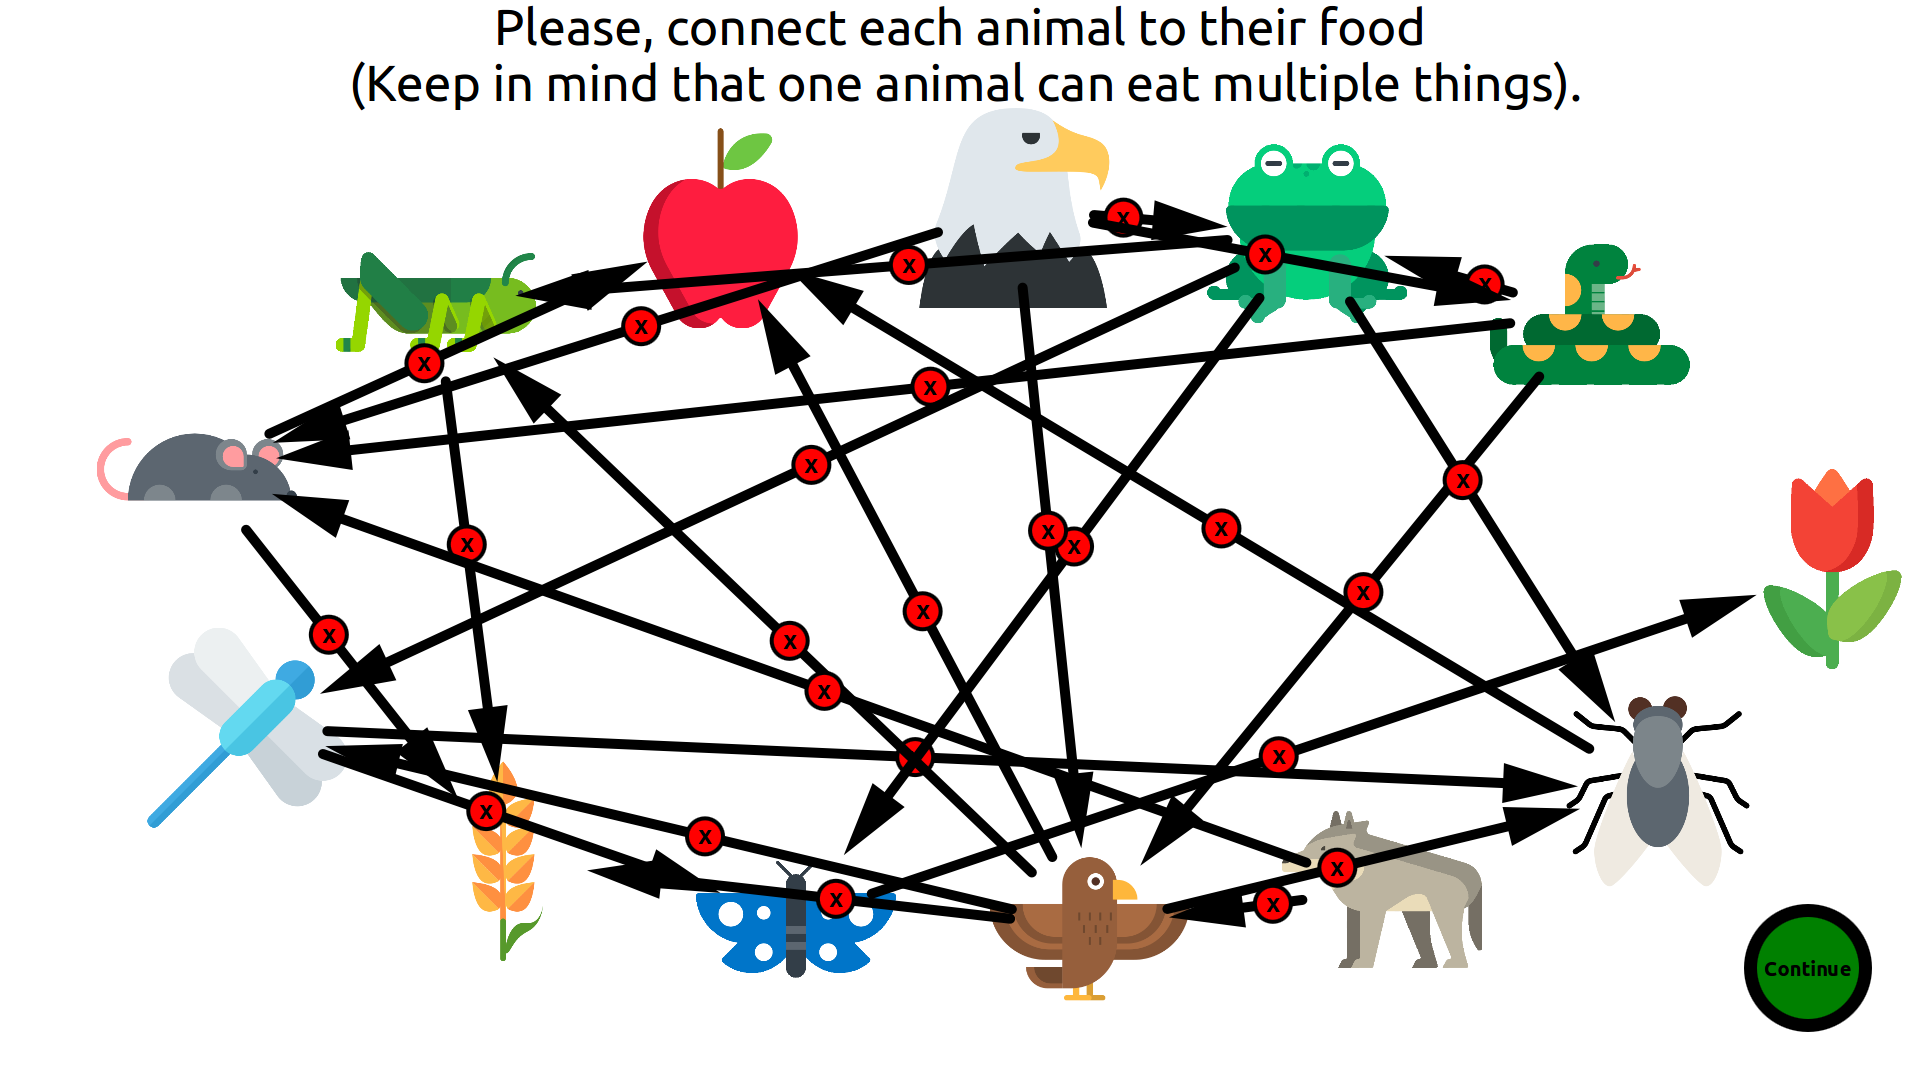
\includegraphics[width=0.95\textwidth]{full_graph.png}
		\captionsetup{width=.95\linewidth}
		\caption{Fully connected test with all the correct connections.}
	\end{subfigure}
	\caption{Test screen to evaluate children's knowledge, empty starting screen (a) and fully connected and correct test (b).}
	\label{fig:test}
\end{figure*}
%\ES{tense?}
They are in total 25 different correct connections and 95 possible incorrect ones. As the child can connect as many arrows as desired, the performance is defined as the number of correct arrows above chance (for the number of connected arrows on the test) divided by the maximum achievable performance, to reach a score bounded to $[-1,1]$. For example, if a child connects 5 good arrows and 3 bad, their performance would be:

\begin{equation}
P=\frac{\#good-(\#good+\#bad) \cdot \frac{total good}{total}}{total good - total good \cdot \frac{total good}{total}} = \frac{5-(5+3) \cdot \frac{25}{25+95}}{25 - 25 \cdot \frac{25}{25+95}}=0.168
\end{equation}
			
The three tests (pre, mid and post interaction) resulted in three performance measures. To account with initial differences of knowledge and the progressive difficulty to gain additional knowledge, we computed the learning gain as the difference between the final and initial knowledge divided by the `progression margin': the difference between the maximum achievable performance and the initial performance. This learning gain indicates how much of the missing knowledge the child managed to gain from the game.
			
\subsubsection{Game Metrics}
Different metrics have been gathered during the game rounds to characterise the children's behaviours:
\begin{itemize}
	\item \textbf{Number of different eating interactions}: number of unique feeding action type ([0,25]).
	\item \textbf{Points}: cumulated sum of animals' energy over the game (typical range [550,1100]).
	\item \textbf{Interaction time}: Duration of game rounds, how long a game lasted until three animals ran out of energy (typical range [.5,3] minutes).
\end{itemize}

The number of different eating interactions informs on how many learning items the children have encountered in the games. A feeding interaction happens when an animal is moved to its food (or to a predator); and the number of different feeding interaction represents how many different unique correct connections the child has been exposed to during the game (multiple feeding actions between the same animals would count only once). A game with a high number of different feeding represents a game where the child had the opportunity to learn many correct connections between animals. Consequently, by increasing this number, the children would be exposed to more learning items which should help them to perform better on the tests. Both the interaction time and the number of points reached in the game inform on the children's success in the task: keeping the animals alive as long as possible and their engagement. 

%Maybe talk about compliance

\subsubsection{Robot Learning}

In the supervised condition, the robot executed actions selected or validated by the teacher, and by using \gls{sparc}, the robot could propose actions to the teacher. Faced with a proposition, the teacher had multiple ways to react. They could accept the action (by waiting for it to be executed, pressing `Do it' or selecting the same action manually) or refuse it (by pressing the `Cancel', `Skip' or `Remove' buttons). As such, actions going through this pipeline can be divided in three categories: actions selected by the supervisor, robot's good propositions and robot's bad propositions. And the evolution of these categories represents how much the online component of the learning improved the quality of the robot's suggestions and reduced the workload on the teacher. 

Some times the teacher cancelled actions and then selected them again, we called this effect the `reselection'. To obtain the final numbers of accepted and refused actions, we removed these reselection from the bad propositions and we added them to the good propositions as it represents cases where the teacher refused an action by accident.

\section{Results}

% and right graphs present the 

%Preliminary results (currently in progress, due to be completed before the submission of the full article) show that (1) the robot is able to effectively jointly learn action and social policies (Figure 2), (2) the learning gains of the children supported by the autonomous robot are not significantly different from the gains when the learning is supported by a robot teleoperated by the human expert, which would indicate the utility of the approach.

Similarly to Chapter~\ref{chap:control}, we analysed the results using Bayesian statistics and the JASP software~\citep{jasp2018}. We used a Bayesian mixed ANOVA as omnibus test to explore the impact of conditions or repetition on the metrics. Additional post-hoc tests use a Bayesian mixed ANOVA comparing the conditions one by one and fix the prior probability to 0.5  to correct for multiple testing.
\afterpage{%
	\clearpage% Flush earlier floats (otherwise order might not be correct)
	%	\thispagestyle{empty}% empty page style (?)
	\begin{table}[ht]
		\centering
		\ra{1}
		\caption{Example of events during the first minute of a round.}
		\label{tab:tuto_round}
		\begin{tabularx}{\textwidth}{@{}L{.2}L{1.8}|L{.2}L{1.8}@{}}\toprule
			Time & Event & Time & Event\\
			\midrule
			4.1 & childtouch frog & 34.4 & childtouch wolf\\
			4.3 & failinteraction frog wheat-3 & 34.7 & \textcolor{SkyBlue}{robot proposes remind rules}\\
			4.9 & animaleats frog fly & 35.0 & animaleats wolf mouse\\
			5.8 & childrelease frog & 36.0 & \textcolor{BurntOrange}{teacher selects wait}\\
			6.6 & \textcolor{SkyBlue}{robot proposes congrats} & 36.0 & animaleats wolf mouse\\
			7.6 & childtouch fly & 37.2 & childrelease wolf\\
			7.6 & \textcolor{BurntOrange}{teacher selects wait} & 37.7 & childtouch grasshopper\\
			8.0 & animaleats fly apple-4 & 38.3 & \textcolor{SkyBlue}{robot proposes congrats}\\
			8.3 & childrelease fly & 41.8 & reset\\
			9.1 & \textcolor{BurntOrange}{teacher selects congrats} & 42.1 & failinteraction grasshopper apple-1\\
			9.1 & childtouch frog & 42.7 & childrelease grasshopper\\
			10.3 & childrelease frog & 42.7 & failinteraction grasshopper apple-1\\
			10.8 & childtouch frog & 44.4 & \textcolor{BurntOrange}{teacher selects mvc mouse wheat-1}\\
			11.2 & animaleats frog fly & 44.6 & robottouch mouse\\
			12.4 & failinteraction frog apple-2 & 44.7 & childtouch butterfly\\
			12.5 & animaleats frog fly & 45.1 & failinteraction butterfly wheat-2\\
			13.2 & childrelease frog & 45.6 & childrelease wheat-1\\
			14.2 & childtouch fly & 45.6 & robotrelease mouse\\
			14.5 & animaleats fly apple-2 & 45.7 & robottouch mouse\\
			14.6 & \textcolor{SkyBlue}{robot proposes encouragement} & 48.9 & robotrelease mouse\\
			15.0 & childrelease fly & 49.3 & childtouch butterfly\\
			15.4 & animaleats fly apple-3 & 49.3 & failinteraction butterfly wheat-1\\
			16.9 & \textcolor{BurntOrange}{teacher selects encouragement} & 49.6 & childrelease butterfly\\
			18.2 & childtouch snake & 50.0 & childtouch mouse\\
			18.4 & failinteraction snake wheat-3 & 50.3 & animaleats mouse wheat-1\\
			18.7 & animaleats snake bird & 51.0 & childrelease mouse\\
			19.6 & animaleats snake bird & 51.1 & animaleats mouse wheat-2\\
			20.5 & childrelease snake & 51.4 & \textcolor{SkyBlue}{robot proposes congrats}\\
			20.6 & failinteraction snake wheat-4 & 52.3 & \textcolor{BurntOrange}{teacher selects congrats}\\
			20.6 & \textcolor{SkyBlue}{robot proposes congrats} & 52.9 & childtouch snake\\
			20.9 & childtouch eagle & 52.9 & failinteraction snake wheat-3\\
			21.1 & animaleats eagle bird & 53.2 & childrelease snake\\
			22.0 & animaleats eagle bird & 53.5 & childtouch mouse\\
			22.4 & childrelease eagle & 53.6 & animaleats mouse wheat-3\\
			23.3 & animaldead bird & 54.4 & \textcolor{SkyBlue}{robot proposes congrats}\\
			23.4 & \textcolor{BurntOrange}{teacher selects mvc dragonfly fly} & 54.5 & animaleats mouse wheat-4\\
			23.6 & robottouch dragonfly & 55.0 & childrelease mouse\\
			26.9 & robotrelease dragonfly & 55.6 & childtouch dragonfly\\
			27.7 & childtouch fly & 56.1 & \textcolor{BurntOrange}{teacher selects wait}\\
			28.0 & childrelease fly & 56.8 & failinteraction dragonfly apple-1\\
			28.4 & childtouch dragonfly & 57.3 & childrelease dragonfly\\
			28.6 & failinteraction dragonfly apple-1 & 57.5 & failinteraction dragonfly apple-1\\
			29.1 & childrelease dragonfly & 58.6 & childtouch grasshopper\\
			29.4 & failinteraction dragonfly apple-1 & 58.6 & failinteraction grasshopper apple-1\\
			30.3 & childtouch dragonfly & 58.8 & childrelease undefined\\
			30.3 & failinteraction dragonfly apple-1 & 59.1 & childtouch dragonfly\\
			30.7 & \textcolor{SkyBlue}{robot proposes encouragement} & 59.1 & failinteraction dragonfly apple-1\\
			31.0 & failinteraction dragonfly apple-1 & 59.2 & failinteraction grasshopper apple-1\\
			31.8 & \textcolor{BurntOrange}{teacher selects wait} & 59.9 & failinteraction dragonfly apple-1\\
			32.5 & childrelease dragonfly & 60.3 & childrelease dragonfly\\
			\bottomrule
		\end{tabularx}
	\end{table}
	\clearpage% Flush earlier floats (otherwise order might not be correct)
}

\subsection{Example of a Session}

Table~\ref{tab:tuto_round} presents an example of the first 50 seconds of a round. Propositions from the robot are in blue, and actions from the teacher in orange. For example, at t=16.9, the teacher accepted the proposition from the robot. Alternatively, in some cases, such as the suggestion at t=20.6, the teacher did not evaluate actions proposed by robot, but just selected another action. In that case, the action proposed is not evaluated and only the selected action is executed and used for learning. In other cases, such as at t=6.6, the algorithm suggested an action, the teacher decided to wait, before selecting it again after a short delay. This is an example of `reselection' as mentioned before. Finally, at t=44.4 seconds, the teacher selected the action to move the mouse closer to the wheat, and after the robot moved the mouse, the child tried other animals and then fed the mouse with the wheat, demonstrating how the actions from the robot could help the children to discover new connections between animals.

%\ES{to remove}

\subsection{Comparison of Policy}

Figure~\ref{fig:tutoring_actions_distribution} presents the number of actions of each types executed by the teacher (in the supervised condition) and the autonomous robot. Both action policies presented similarities: the action `Move away' was almost never used, `Move to' was never used, and the supportive feedback (`Congratulation' and `Encouragement') were used more often than `Remind rules' or `Drawing attention'. However, some dissimilarities were also present, for instance, the autonomous robot used more encouragements than congratulations while the teacher did the opposite. The autonomous robot also reminded the rules more often and used the `Move close' action less than the supervisor. These differences of actions are probably linked to the type of machine learning used; with instance based learning, some datapoints will be used in the action selection much more often than others, which might explain these biases. But these results show that the robot managed to learn a social and technical action policy presenting similarities with the one displayed by the teacher providing partial support for H2.

\begin{figure}[ht]
	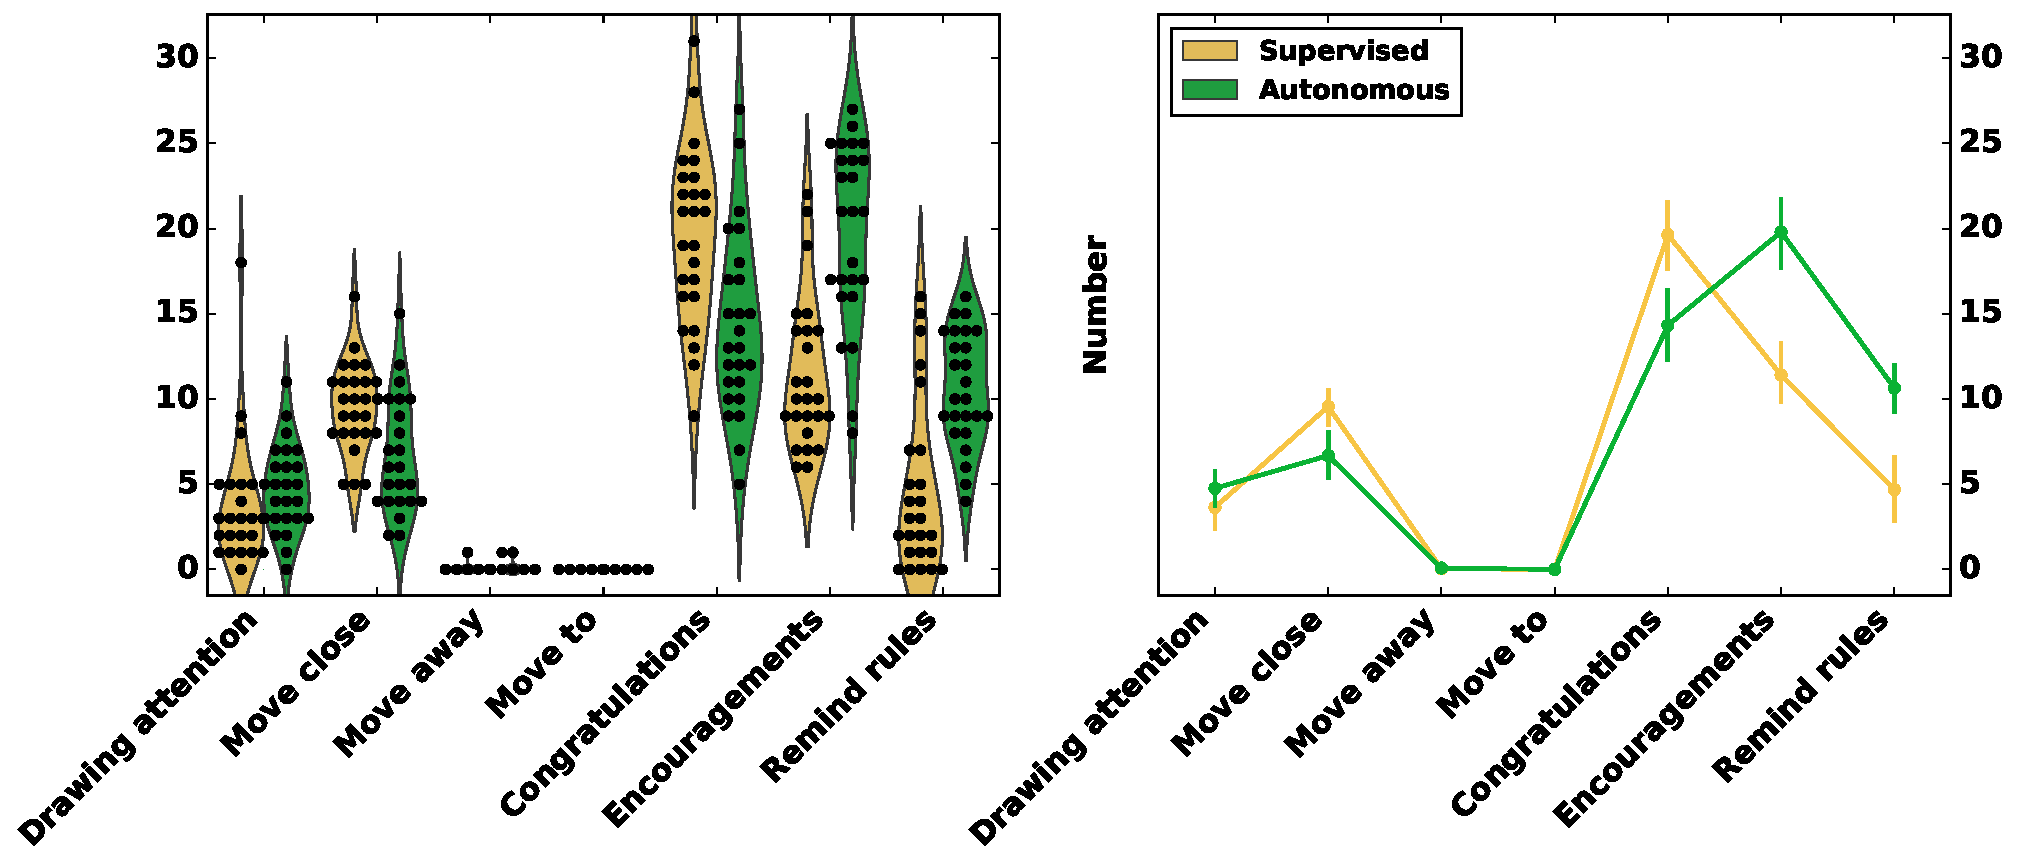
\includegraphics[width=1\linewidth]{actions.pdf}
	\centering
	\caption{Comparison of distribution of actions executed by the robot in the autonomous and supervised conditions. The left graph is a violin plot of the data, while the right presents the means and the 95\% Confidence Intervals}
	\label{fig:tutoring_actions_distribution}
\end{figure}


%\begin{figure}[ht]
%	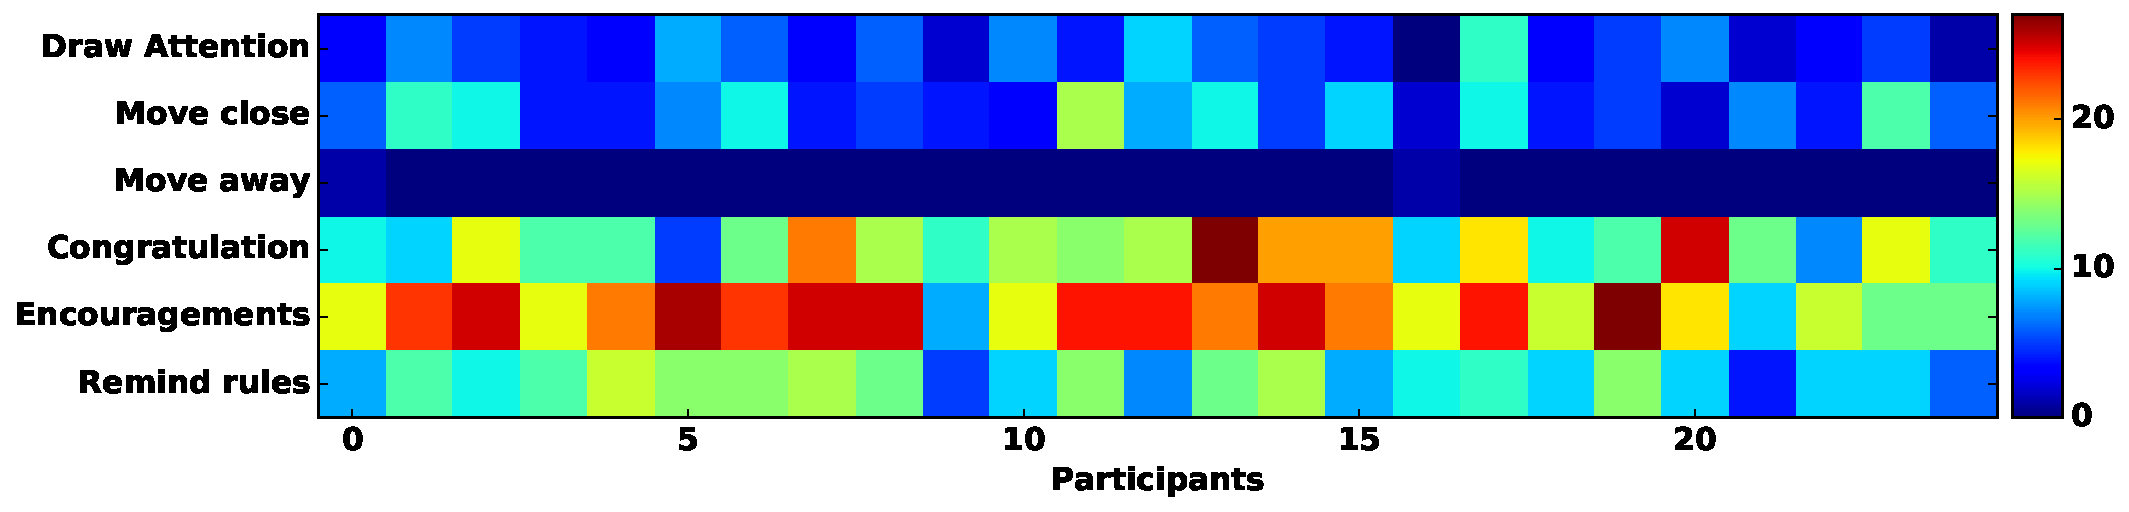
\includegraphics[width=1\linewidth]{autonomous_actions.pdf}
%	\centering
%	\caption{Repartition of actions across the participants in the autonomous condition.}
%	\label{fig:tutoring_autonomous_actions}
%\end{figure}
%
%\begin{table}[ht]
%	\centering
%	\caption{Repartition of action in the policy for both conditions (in \%).}
%	\label{tab:tutoring_policies}
%	\begin{tabularx}{\textwidth}{@{}lYYYccY}\toprule
%		& Draw \newline Attention & Move \newline close & Move \newline away & Congratulation & Encouragements & Remind \newline rules \\
%		\midrule
%		Supervised & 6.6  & 22.2 & 0.1 & 43.1 & 22.7 & 5.3 \\
%		Autonomous & 8.5 & 11.8 & 0.1 & 25.4 & 35.2 & 18.9\\
%		\bottomrule
%	\end{tabularx}
%\end{table}


\subsection{Test Performance}

Figure~\ref{fig:tutoring_performance} shows the evolution of children's performance across the three tests. A Bayesian mixed-ANOVA showed that in all conditions, children's performance increased across the tests ($B=1.5$x$10^{12}$), however the impact of the condition on the learning was inconclusive with a tendency to show no impact ($B=0.539$). This indicates that by being involved in the task, every children learned and improved their performances on the test (by gaining in average 13\% of the missing knowledge), but the robot behaviour during the game did not have an important impact on the children's learning gain (see Figure~\ref{fig:tutoring_learning}), invalidating H3. %\ES{should I discuss the inhomogeneity of the population, wide variation of P1}

\begin{figure}[ht]
	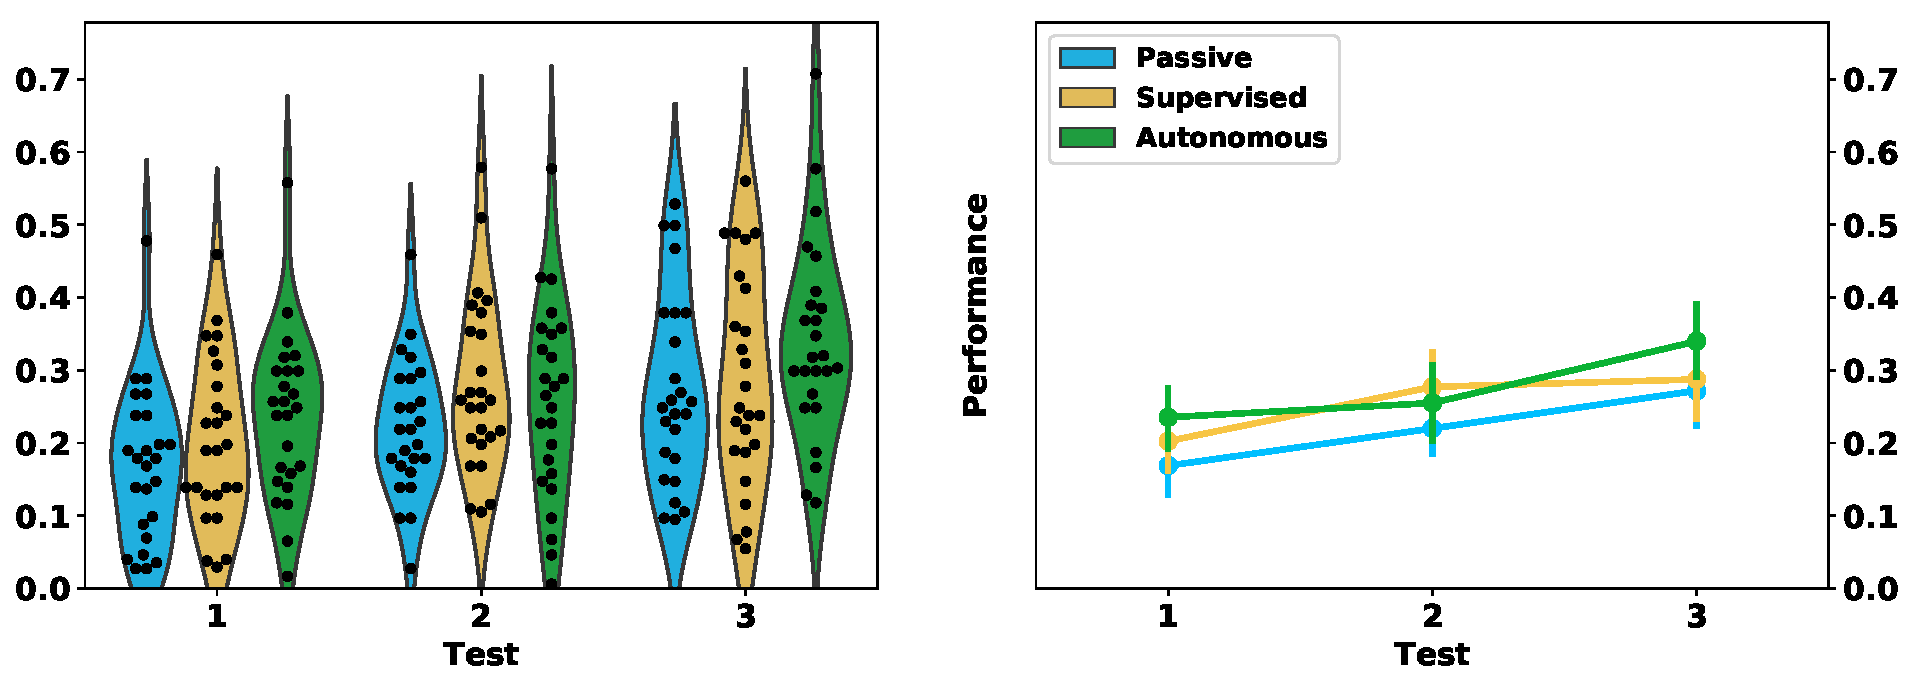
\includegraphics[width=1\linewidth]{perf.pdf}
	\centering
	\caption{Children's performance for the three tests: pretest, midtest and posttest for the three conditions.}
	\label{fig:tutoring_performance}
\end{figure}

\begin{figure}[ht]
	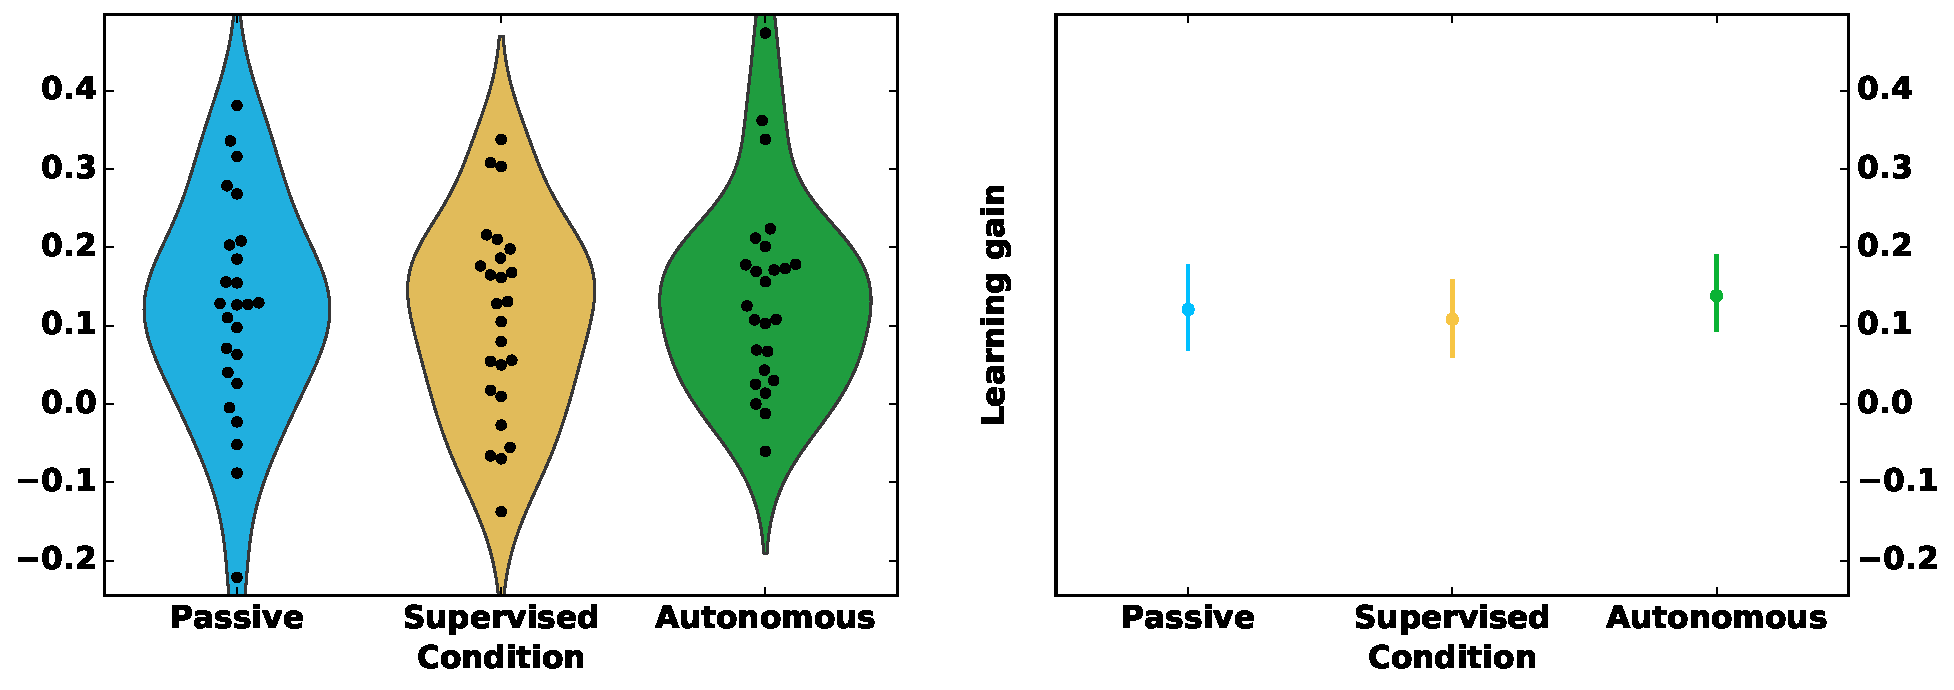
\includegraphics[width=1\linewidth]{learning.pdf}
	\centering
	\caption{Children's normalised learning gain after interacting with the robot for the three conditions.}
	\label{fig:tutoring_learning}
\end{figure}

\subsection{Game Metrics}

\paragraph{Different eating behaviours}
Figure~\ref{fig:tutoring_d_eat} shows the evolution of the number of different eating behaviours exhibited by the children across the four game rounds. A Bayesian mixed-ANOVA showed an impact of the condition on the number of different eating behaviours produced by the children in the game ($B=6.1$). Post-hoc tests showed the absence of difference between the supervised and the autonomous conditions ($B=0.154$), whilst differences were observed between the supervised and the passive condition ($B=512$) and between the autonomous and the passive conditions ($B=246$). This indicates that, compared to the passive robot, the supervised robot provided additional knowledge to the child during the game, allowing them to create more useful interactions between animals and their food, receiving more information from the game potentially helping them to learn. And the autonomous robot managed to recreate autonomously this effect without the presence of a human in the action selection loop.

\begin{figure}[ht]
	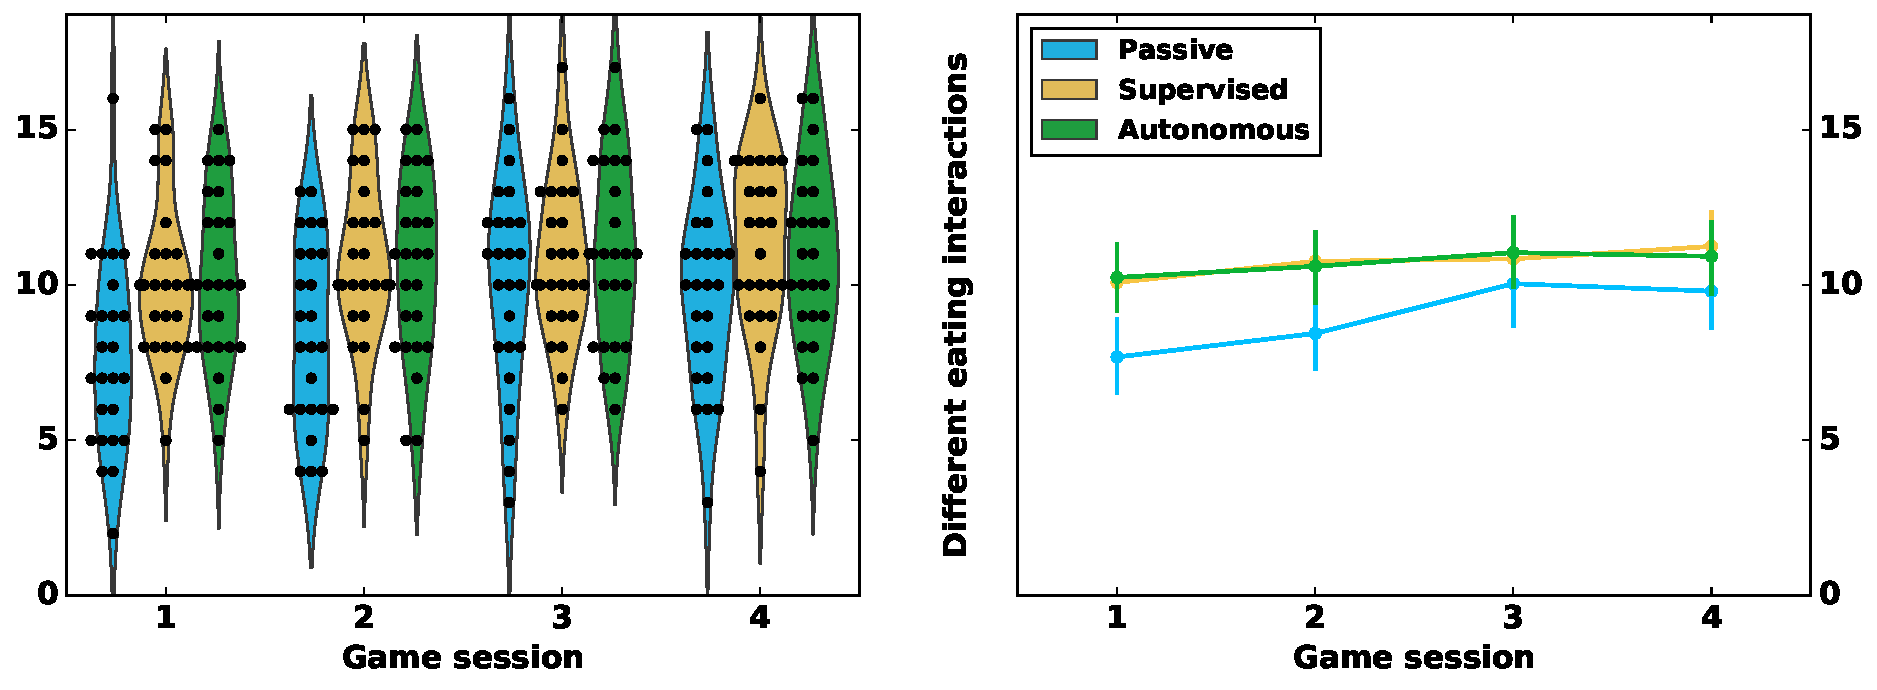
\includegraphics[width=1\linewidth]{d_eat.pdf}
	\centering
	\caption{Number of different eating behaviour for the four games for the three conditions.}
	\label{fig:tutoring_d_eat}
\end{figure}

\paragraph{Points}

Figure~\ref{fig:tutoring_points} shows the evolution of the number of points achieved by the children across the four game rounds. A Bayesian mixed-ANOVA showed an impact of the condition on the number of points achieved by the children in the game ($B=10.2$). Post-hoc tests showed a strong difference between the passive and the supervised conditions ($B=5.1$x$10^4$) and differences between the supervised and the autonomous conditions ($B=5.2$) and the autonomous and the passive condition ($B=5.9$). This indicates that when the robot was supervised, it allowed children to achieve more points than a  passive robot. And a similar effect was observed when the robot was autonomous, however the autonomous robot did not manage to reach the same efficiency as the supervised robot in helping the children to achieve a high score in the game.

\begin{figure}[ht]
	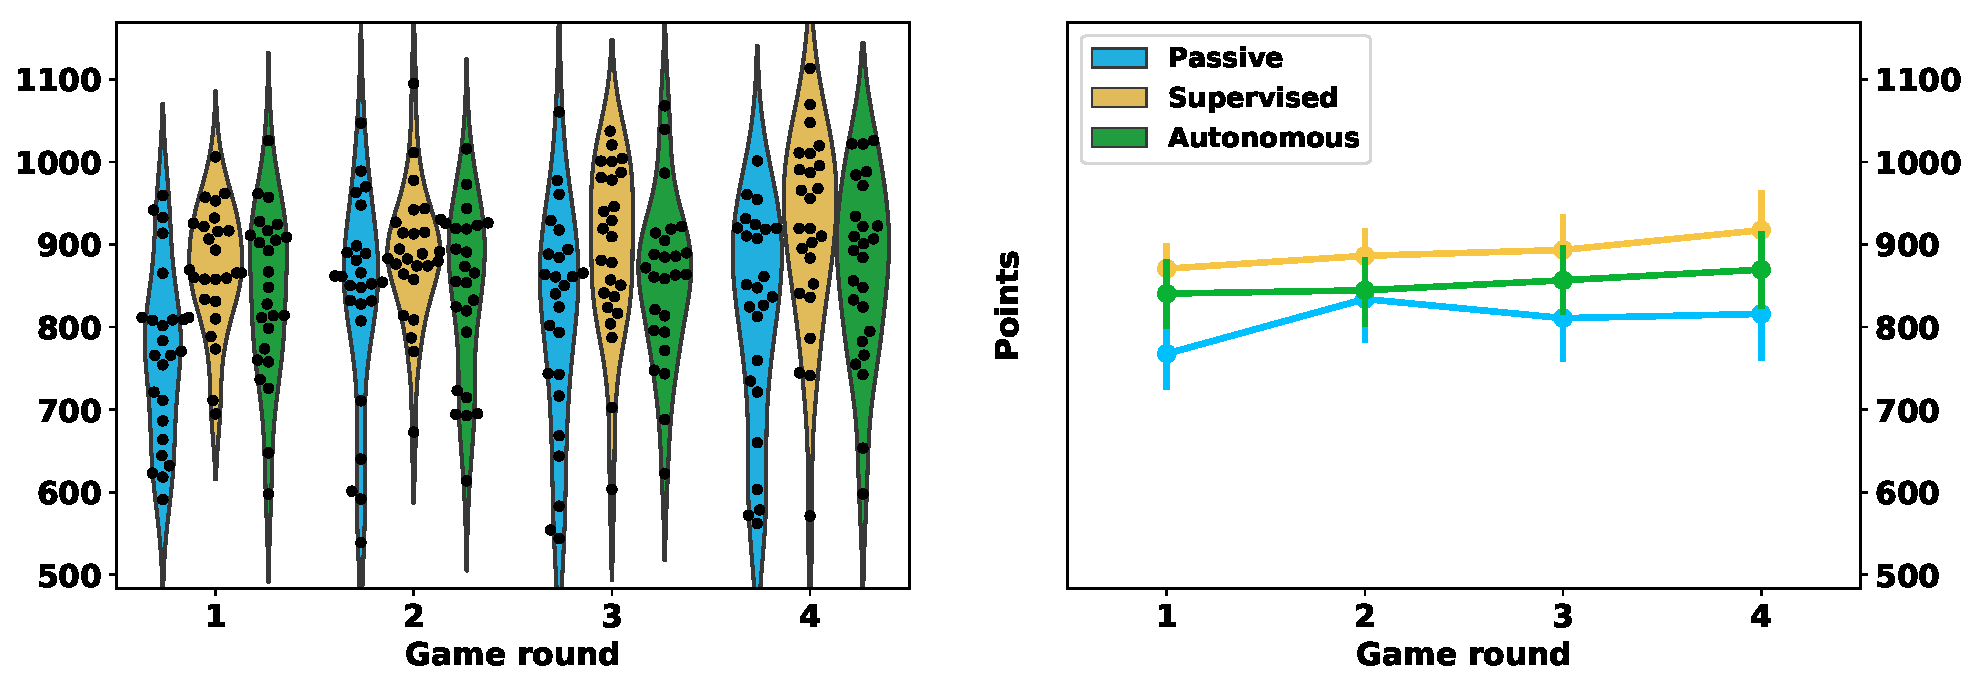
\includegraphics[width=1\linewidth]{points.pdf}
	\centering
	\caption{Points achieved by the children in each game round for the three conditions.}
	\label{fig:tutoring_points}
\end{figure}

\paragraph{Time}

Figure~\ref{fig:tutoring_time} shows the evolution of interaction time across the four game rounds. A Bayesian mixed-ANOVA showed inconclusive results on the impact of the condition on the interaction time in the game ($B=1.1$). However, post-hoc tests showed the absence of difference between the supervised and the autonomous conditions ($B=0.287$), whilst differences are observed between the supervised and the passive condition ($B=118$) and a tendency of difference between the autonomous and the passive conditions ($B=2.9$). This indicates that the supervised robot allowed children to be better at the game, allowing them to maintain animal alive longer than a passive robot. And the autonomous robot learned and applied a policy tending to replicate this effect and without exhibiting differences with the supervised one.

\begin{figure}[ht]
	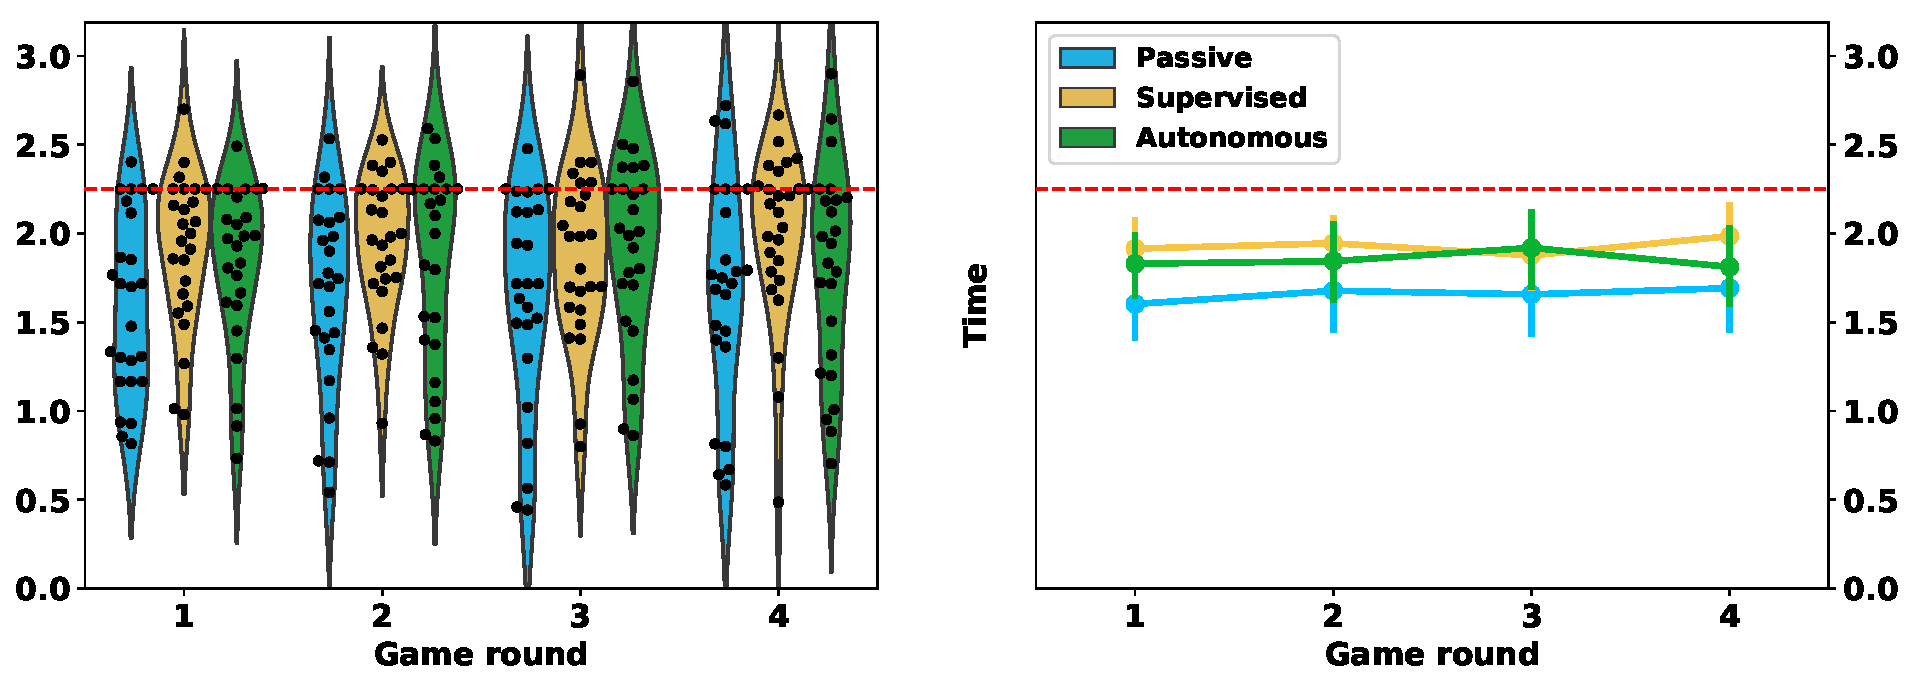
\includegraphics[width=1\linewidth]{time.pdf}
	\centering
	\caption{Interaction time for the four games for the three conditions.}
	\label{fig:tutoring_time}
\end{figure}


\paragraph{Summary}

These game metrics showed that the action policy executed by the autonomous robot allowed children to achieve similar results in the game than when the robot was supervised, and better results than when interacting with a passive robot. This provides support for H2 ("The autonomous robot is able to interact socially and efficiently during the game rounds and maintain the child's engagement during the learning task"). 
%However, children learned similarly in the three conditions, so these improvements in the game did not transfer to improvements in the test neither for the supervised robot nor the Autonomous one. This does not support H1 ("The robot support child learning: learning gain in passive condition $<$ learning gain in autonomous condition $<$ learning gain in supervised condition")

\subsection{Teaching the Robot}

Figure~\ref{fig:tutoring_supervision} presents the reaction of the teacher to the robot's suggestions across all the supervised interactions. Unlike our expectations, the number of correct and bad suggestions as well as teacher selections stayed roughly constant through the interactions with the children. In average, the robot proposed 17.2 (SD=4.0) actions accepted by the teacher and 41.7 (SD=11.1) refused by the teacher per interaction. And the teacher selected manually 25.8 (SD=5.8) actions per interaction. These unexpected results are discussed in details in Section~\ref{sec:tutoring_disc_learning}.

\begin{figure}[ht]
	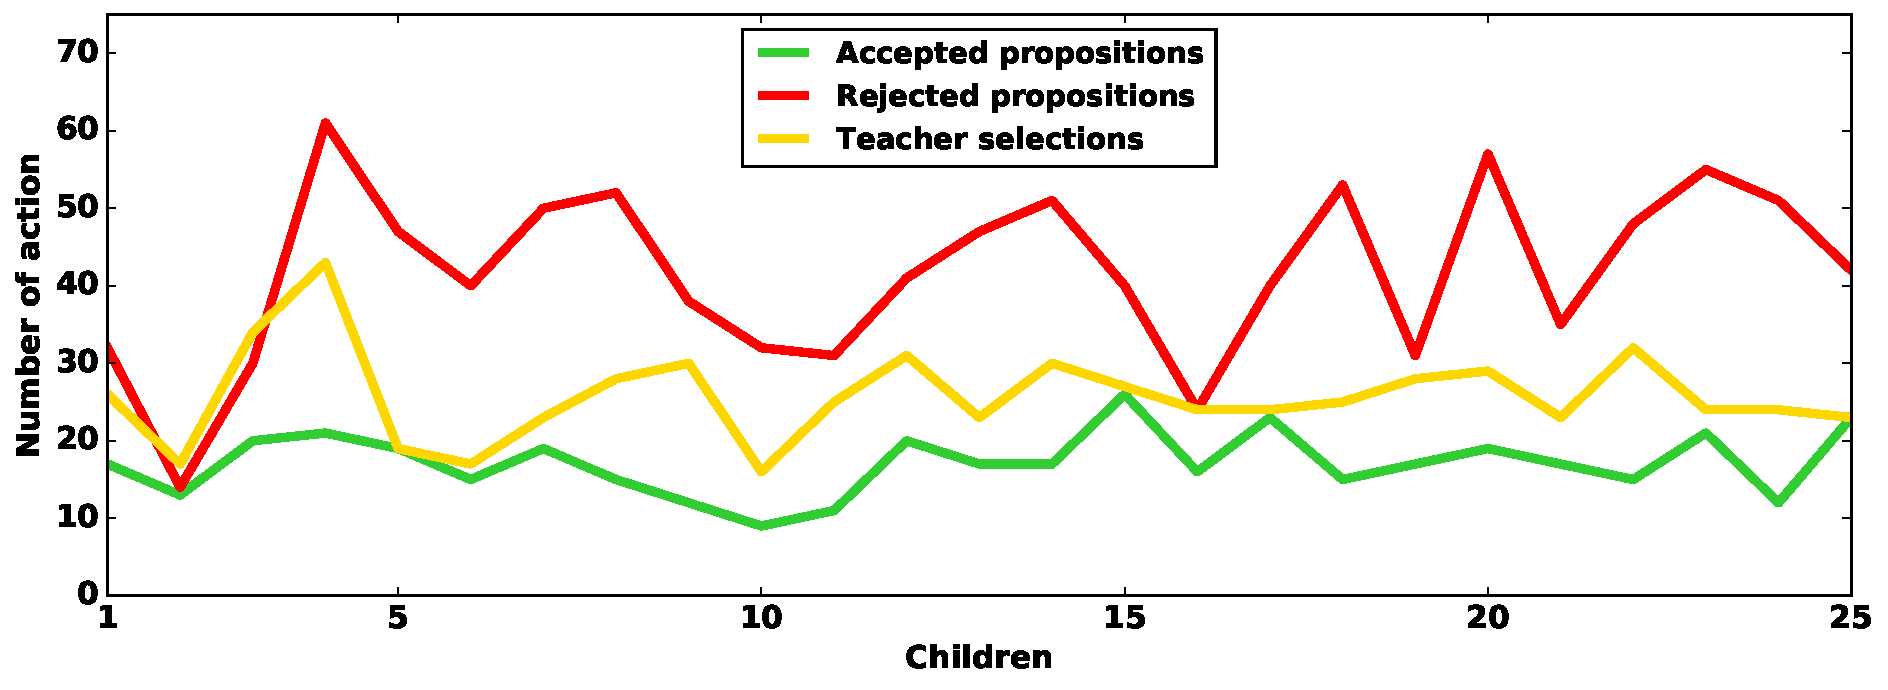
\includegraphics[width=1\linewidth]{./summary_supervision.pdf}
	\centering
	\caption{Summary of the action selection process in the supervised condition: the `teacher selection' label represents each time the teacher manually selected an action not proposed by the robot.}
	\label{fig:tutoring_supervision}
\end{figure}


Figure~\ref{fig:tutoring_actions} presents the accumulated number of different actions in the policy the teacher used. We can observe a sharp increase in the first 5 interactions, when the teacher used the main actions for the first time. Then there is a mixture of small plateaus and small increases, indicating that the teacher alternated phases where she enriched her action policy and phases where she maintained her policy. And finally, the number of different actions in the policy seems to converge around 60 toward the last interactions.

\begin{figure}[ht]
	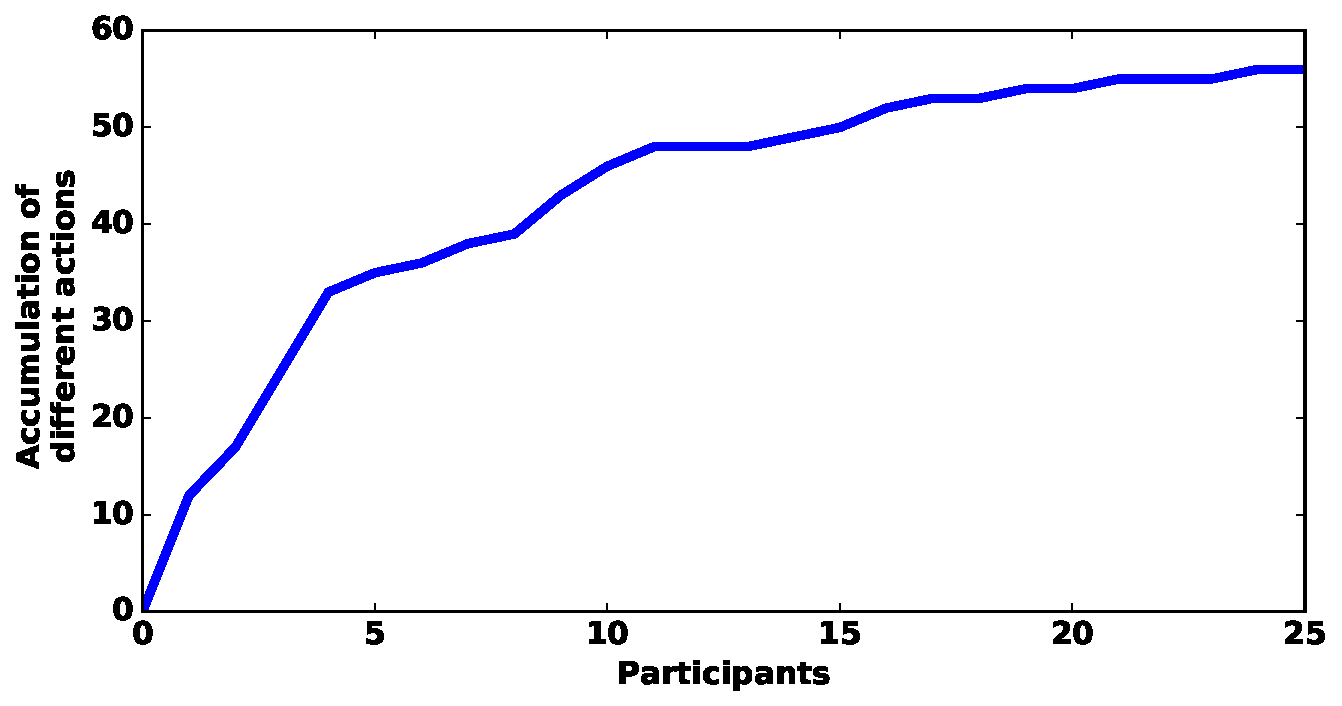
\includegraphics[width=.85\linewidth]{./number_actions.pdf}
	\centering
	\caption{Number of different actions used by the teacher throughout the interactions with the children.}
	\label{fig:tutoring_actions}
\end{figure}


In post-hoc discussion, the teacher reported three phases in her teaching: 
\begin{itemize}
	\item First sessions: she was not paying much attention to the suggestions, mostly focusing on having the robot executing a correct action policy.
	\item Sessions 6 to around 16: she was paying more attention to the suggestions without giving them much credit.
	\item Last sessions: she started to trust the robot more but without ever trusting it totally.
\end{itemize}

%\ES{I should add more about it...}
Appendix~\ref{app:diary} presents a more detailed diary of the teacher throughout her supervision. Additionally, while the buttons cancel and skip has different impact of the learning, and were designed to be used in different cases, the teacher reported that she used them interchangeably.

The teacher did report a decrease of workload as she she progressed in the sessions number. This was supported by behaviours such as typing her observations on a laptop, while gazing at the interface in multiple interactions (especially at the start of a round). However, as shown by the evolution of curves in Figure~\ref{fig:tutoring_actions}, this decrease of workload seemed to be due mostly due to the teacher getting used to the interaction, and not to the online learning and the improvement of the suggested proposition, invalidating H4.

%Figure~\ref{fig:tutoring_proposition} presents the reaction of the teacher to the robot's suggestions across all the supervised sessions. In average the teacher accepted 22.3\% of all the proposition of the robot (by enforcing the action, let it be executed or using the `Do it' button), which represents 35\% of the actions executed by the robot. This effect tends to be stable across the sessions. The teacher interaction pattern evolved overtime, such as by using mostly the `Cancel' button in the start then the `Skip' one, but in the end, the teacher used this two buttons mostly interchangeably even if the algorithm underlying reaction is different. Another observation is the evolution from using the auto-execution function to the `Do it' button once the teacher felt more comfortable in the supervision. The teacher reported three phases in her teaching: 
%
%\begin{itemize}
%	\item First sessions: she was not paying much attention to the suggestions, mostly trying to have the robot executing a correct action policy.
%	\item Session 20 to around 65: she was paying more attention to the suggestions without giving them much credit.
%	\item Last sessions: she started to trust the robot more but without ever trusting it totally.
%\end{itemize}
%
%\begin{figure}[ht]
%	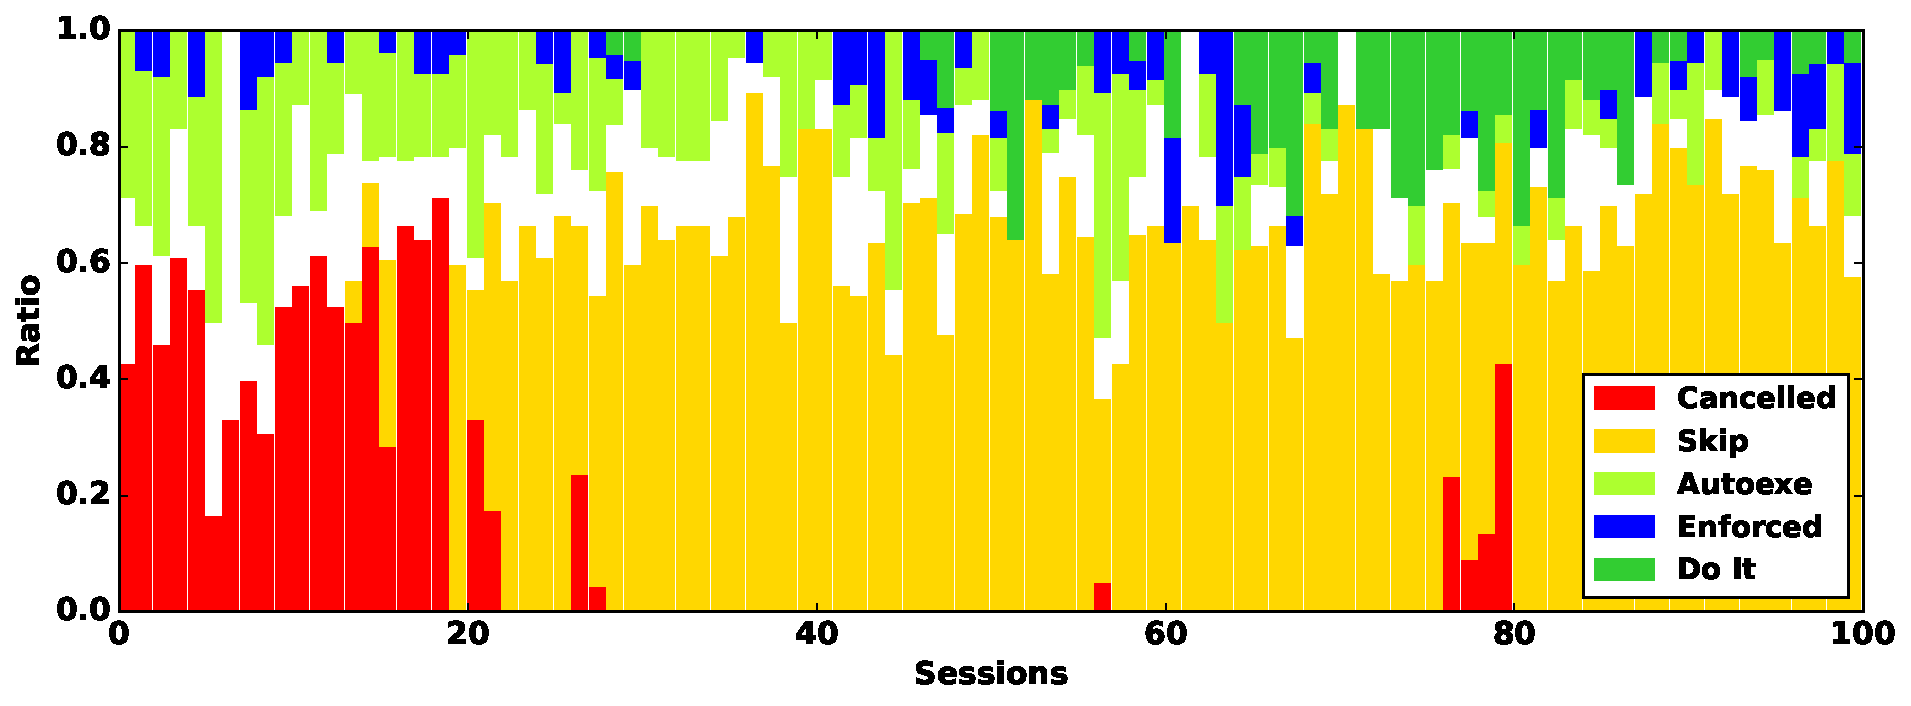
\includegraphics[width=1\linewidth]{propositions.pdf}
%	\centering
%	\caption{Teacher's reaction to the robot's propositions along the sessions.}
%	\label{fig:tutoring_proposition}
%\end{figure}
%
%
%\begin{figure}[ht]
%	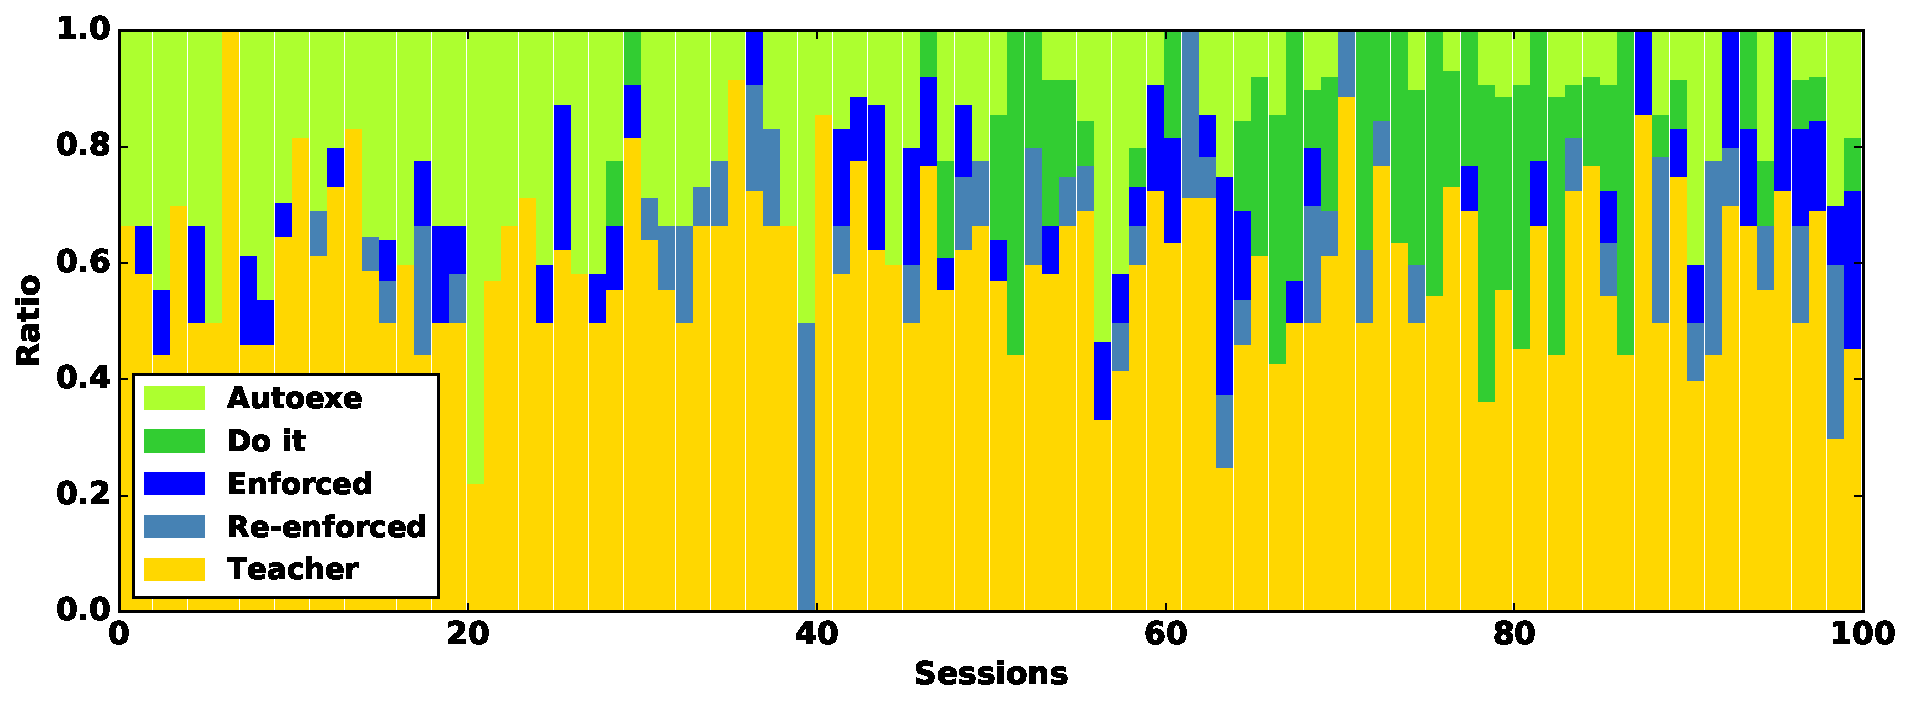
\includegraphics[width=1\linewidth]{selections.pdf}
%	\centering
%	\caption{Origin of the actions executed by the robot. Re-enforced actions indicates that an action has been selected after having been cancelled or skipped by the teacher.}
%	\label{fig:tutoring_selection}
%\end{figure}
%
%Additional comments:
%\begin{itemize}
%	\item The robot proposed in average 58\% more actions than the number of actions selected by the teacher.
%	\item As the time is continue and not discrete, the concept of correct actions is shifted, and actions selected by the teacher might have been proposed by the robot a fraction of second later without being counted as good proposition.
%	\item The teacher often cancelled/skip actions directly as they arrived without taking time to analyse them (limitation of this implementation of SPARC).
%	\item Evolution of teaching policy limits the potential of learning (not one single policy applied by the teacher, but an evolving one).
%	\item Children are different, so the teacher tried to apply different action policy for each child.
%\end{itemize}
%
%
%\begin{figure}[ht]
%	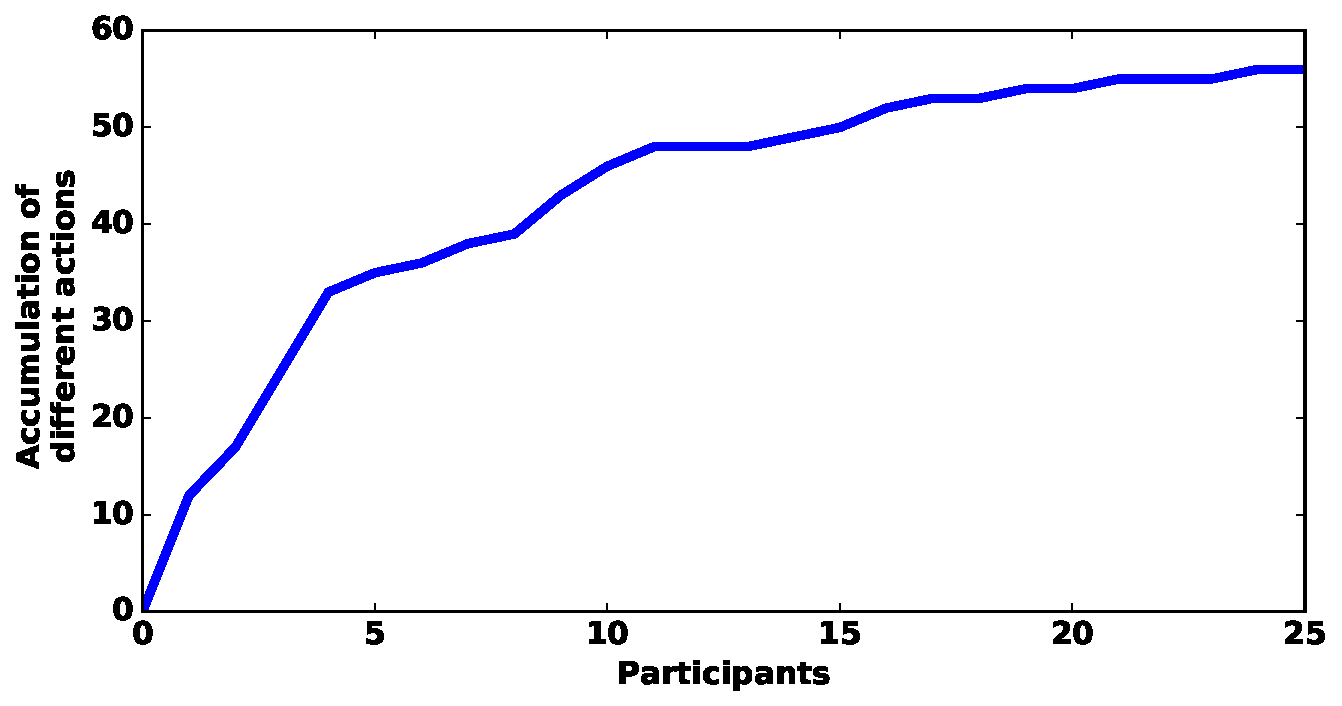
\includegraphics[width=.6\linewidth]{number_actions.pdf}
%	\centering
%	\caption{Accumulation of the number of different actions used by the teacher across the  participants.}
%	\label{fig:tutoring_actions}
%\end{figure}


\section{Discussion} \label{sec:tutoring_discussion}

This study explored if a human could teach a robot to support a child in a educational game. This resulted into two subquestions: ``can a robot be taught safely an interactive policy?'' and ``would the resulting autonomous policy support the child in the game?''. These two questions were addressed by comparing three conditions. The first one, the passive condition corresponded to a robot not providing any feedback during the game and was used as the baseline. In the supervised condition, a human taught the robot to interact with the child using \gls{sparc}; and in the autonomous condition, the robot applied the policy learned in the supervised condition to interact with the child without supervision.

The main findings are that the autonomous robot demonstrated an action policy similar to the one used by the teacher when supervising the robot, and both these policies had positive effects on the child compared to the passive robot. However, these positive effects in the game did not transform into learning gain in the tests. Additionally, when the robot was supervised, the number of actions manually selected by the teacher and the number of correct and incorrect actions proposed by the robot remained consistent through the different interactions.

\subsection{Children Behaviours and Learning Gain}

The active robots' behaviour encouraged children to produce more `useful' behaviours during the interaction. When interacting with an active robot, children encountered more situations with learning potential (such as the different eating behaviours). However, this additional exposure to learning items did not transform into an increase in learning gain in the test. In the three conditions, the children had similar test scores; thereby not supporting H3. We identified two possible causes for this absence of transfer between game behaviours and performance in the test. The first is that the game by itself, without the robot, encouraged the children to explore, and interacting independently with it was sufficient to promote learning. As such, in the active conditions, the robot's behaviour might have distracted children from their exploration or encouraged them to rely on the robot rather than their own exploration. In that case two effects might have cancelled each other out: on one hand the behaviour of an active robot provided additional knowledge to the child, but on the other hand the same behaviour might have perturbed children's exploration of the game, potentially reducing their learning. This might explain the absence of any effect of the robot's behaviour on the children's performance. The second possible explanation would be in that the test itself might not have been able to capture the child's knowledge accurately. The test only asked children to connect as many animals as possible. However it might have been too open-ended, and might not have encouraged children to make all the connections they knew to be correct, but simply to make an arbitrary number. %In that case, the test would not represent the real knowledge of children, but only be a lower bound. 
Having forced-choice questions, for instance randomly selecting 20 connections and asking children if they are correct, might have provided a better evaluation of the children's knowledge. Additionally, the test did not include feedback on right/wrong answers, thereby the children were not given immediate reinforcement for correct connections.

%By only asking children to connect the animals they know, we do not force them to make a choice. They have the opportunity to stop the test at any time. This might limit the efficiency of the comparison as some children might continue further than other, and we might miss some knowledge about the children. It might have been better to select randomly 20 connections between the animals and ask the children if one animal can eat the other.

%\begin{itemize}
%	\item Game self-exploratory, robot behaviour might distract the children
%	\item no correlation between exposure to learning items and learning gains
%	\item Limits of the knowledge test: too open-ended, might have been better to have 10 random animals selected and ask the child to say yes/no?
%	\item Limit of the performance calculation: the test was probably not able to capture the exact knowledge of children - Learning is about discovering interactions
%\end{itemize}

\subsection{Human in Control}\label{sec:tuto_control}

As demonstrated by Figure~\ref{fig:tutoring_actions_distribution}, in the supervised condition, the robot only executed actions relevant to the current game. For example, the actions `move away' and `move to' were rarely used possibly because they could be unsettling for the child. Similarly, Figure~\ref{fig:tutoring_supervision} shows that the teacher could use \gls{sparc} to prevent undesired actions being executed by the robot. As such, H1 (``In the supervised condition, \gls{sparc} allows the teacher to teach the robot while ensuring its behaviour is constantly appropriate.'') is supported. By having the robot proposing actions before executing them, \gls{sparc} allows teachers to ensure that the robot's behaviour is appropriate even during the learning phase, thus enabling robots to learn \emph{in situ} in complex and sensitive environments.

\subsection{Robot Learning} \label{sec:tutoring_disc_learning}

One of the motivation for \gls{sparc} is to provide a way to smoothly move away from \gls{woz} to \gls{sa}, potentially leading to pure autonomy. By learning the action policy online, the number of actions selected or corrected by the teacher should decrease and the number of accepted suggestions should increase, hence reducing the teacher's workload. However, this expectation (and by extension H4) was not validated by this study's observations. The number of actions accepted, refused and selected by the teacher remained consistent throughout the interactions. We identified five potential explanation for this differences discussed below.

\paragraph{Suggestion rate too high.}

The first explanation is that the robot proposed a large number of actions (58\% more than the total number of executed action). This indicates that the adaptive threshold restricting actions to be proposed was consistently low. This high number of proposed actions partially explains the high number of actions refused by the teacher. Unstructured interviews with the teacher after the study revealed that as the robot tended to propose actions at high frequency, the teacher reached a point in her supervision where she often preferred refusing the robot's propositions even in cases where they were correct rather than taking the time to evaluate them and risk having undesired actions executed. 

\paragraph{Human adaptation.}

A second effect which may have limited the correctness of the propositions is the evolution of the teacher's policy. As the teacher progressed in the interactions, she increased the complexity of her action policy, adapting it to each child and using a wider variety of actions. Having this kind of moving target for learning limited the maximal performance achievable by the algorithm. Additionally, as the algorithm only proposed actions already used at least once, this led to a requirement on the teacher to select each action enough times to inform the algorithm of when they should be selected. However, towards the end of the teaching phase, the number of different actions used by the teacher tended to converge. This indicates that the algorithm might have achieved better results at predicting the teacher's actions if the teaching phase had been extended.

\paragraph{Continuous time.}

This study also stood out from classic problems using \gls{ml} on another point. In this study, the agent interacted in real-time, whereas generally agents using \gls{ml} only exist in a discrete time. In classical \gls{mdp} frameworks, an action has to be selected at each step, actions last one step, and optimal strategies might exist. However, when interacting in the real world, actions take many steps and in most time steps no action should be selected. Additionally, due to the continuous side of the time, actions are not valid at a specific step, but around that step. This implies that to reduce the teacher's number of selected actions, the algorithm does not have to select the same action as the teacher at each step, but needs to anticipate the teacher's actions, so that the teacher does not select them first. The algorithm might select a correct action around the time the teacher would select it, but if that proposition arrived a step after the teacher's selection, it would not be considered as a good proposition. This might explain the limited visibility of the results. 

\paragraph{Algorithm.}

Another element potentially explaining the limited efficiency of the online learning is related to the algorithm itself. In its simplest form (and as used in this study), nearest-neighbours considers only one neighbour, making it highly sensitive to outliers. Consequently, some instances in memory could be used too often, leading to an imbalance of policy (as observed when comparing the autonomous and supervised policy). One way to tackle this issue could be to use the k nearest neighbours instead, this might have led to a more robust learning algorithm. 

%\ES{clarify: especially temporal relations to the other part}
\paragraph{Difference of state representation between human and robot.}

Finally, in such complex tasks, humans are making use of a large number of `states', such as temporal relations between events, to select actions. If the state definition the robot uses does not contain or cannot cope with these features, the learning will be limited. As mentioned in Section~\ref{ssec:back_lfd}, \cite{knox2014learning} and \cite{sequeira2016discovering} stress the fact that a human teacher (or demonstrator) should have access to the same features as the algorithm to increase transferability. However, even when this recommendation is met, the teacher can create temporal structures which may not be available to the algorithm (especially an instance-based one), reducing the potential for learning the teacher's policy exactly. In this study, for methodological reasons, we did not remove the teacher from the room when the child interacted with the robot. Consequently, this allowed the teacher to have access to features of the interaction absent from the state representation used by the algorithm. For example, the teacher sometimes used the results from the tests (initial and mid) to inform her action policy. However these features were not available to the robot, which might have limited the learning. Additionally, in this study, the teacher did not use `complex' feature selection, she mostly used the minimum number of features required for an action to be unambiguous even if she might have used other features for her decision. One example of a complex action would be to indicate to the child the food of the animal they are currently touching. To inform the algorithm that the animal being touched by the child matters, the teacher would need to select the animal touched by child while selecting the `drawing attention' action for its food. Whilst being possible, this feature of the teaching was a bit complex to use on the interface, and was not used by the teacher in this study, potentially preventing the algorithm from having access to the exact set of features used by the teacher when selecting an action.

%Additionally, some of the feature used by the teacher to decide which type of policy to apply might not be available to the algorithm (for instance temporality or verbal utterance in our case). This implies that the algorithm might receive different demonstrations (outputs to match) for the same inputs, complexifying further the learning process.

%\ES{with more training data, and an algorithm addressing the fixable issues, the autonomous policy and the supervised ones should become closer and the workload on the teacher might decrease as the robot learns}

\paragraph{Summary}

While the autonomous behaviour was different from the supervised behaviour, both policies still presented many similarities in the distribution of actions executed by the robot and the children's reactions to the behaviours. Additionally, the challenge of learning a suitable action policy for the robot should be highlighted: the state space was large, continuous and the action space contained a large number of possibilities and the interaction was social and multimodal. Finally, the algorithm was not provided with any `innate' information, all the dimensions of the state or the actions were treated the same way, the semantics of the interaction were inferred from the demonstrations and feedback. With more training data and an improved algorithm, the robot learning could have been more efficient and might have led to a decrease in workload for the teacher and an increased similarity between the the teacher's policy and that of the autonomous robot. 
%\ES{discuss the stopping point - and complexity of the task: continuous, multimodal... + large space without semantic included}

%\ES{Good results could be achieved autonomously only if initial knowledge was hard coded in the state action space}

\subsubsection{Stopping condition}

During this study, each condition consisted of 25 children. This means that the robot learning was terminated at some point without possibility to refine its action policy further, and this conditioned all the results observed in the autonomous condition. By involving more children in the supervised condition, the teacher's action policy might have converged, the learning algorithm might have increased its performance by suggesting more appropriate actions to the teacher and potentially reducing her workload. This relatively arbitrary cut-off of the learning phase had important effects on both the supervised and autonomous conditions, and continuing with more children or stopping earlier might have lead to dramatically different results.

\subsection{Importance of the Teacher}

\gls{sparc} includes two distinct but simultaneous human-robot interactions. Thus, evaluating such interconnected interactions is a complex task as each human's behaviours impacts the other's. To explore in a repeatable and comparable manner one of the interactions, the other one needs to be as consistent as possible. However, humans are not consistent and, consequently, evaluating these two interactions simultaneously is a challenge. By deciding to keep the same teacher for all the interactions, we only have a sample of one participant as a robot teacher. As a result, this study is in essence a case study of one participant teaching a robot to interact with children; and this could have created some biases in the supervision. As seen in previous chapters, different humans would teach the robot differently. It would have been interesting to explore this axis, by introducing distinct teachers and observing how their different behaviours impacted the learning process and the final policy. We would expect that the resulting autonomous behaviours should match the each teacher' policy. However due to the variability of children, a large number of participants would be required to evaluate a robot's learning from several teachers. As such, we did not evaluate more than one teacher in this study.
%to the number of children required to train and test the robot, we could not do it. 
%\ES{develop more children's variability}
%
%As such, this could create some biases in the supervision, but as the teacher was not aware of the learning mechanism used for the robot and was not provided feedback on how to interact with the robot, these biases were limited. 
%\begin{itemize}
%	\item evolve their action policy
%	\item we had to fix her, so another teacher would have behaved differently
%\end{itemize}


%\begin{itemize}
%	\item The robot proposed in average 58\% more actions than the number of actions executed by the robot (approved and selected by the teacher): the threshold to select actions was probably too low, leading to too many propositions and the adaptivity of the threshold not good enough
%	\item As the time is continuous and not discrete, the concept of correct actions is biased, there is no `correct' action policy associating an action to each time steps. Additionally the timing of the proposition was key as actions proposed just after a selection would have been discarded.
%	\item To reduce the number of teacher selection, the robot would need to \emph{anticipate} every single teacher's action: not only knowing what action to do, but suggesting it the teacher before she started executing the action.
%	\item The teacher often cancelled/skip actions directly as they arrived without taking time to analyse them (limitation of this implementation of SPARC).
%	\item Evolution of teaching policy limits the potential of learning (not one single policy applied by the teacher, but an evolving one, including more actions as the teacher is more comfortable with the system).
%\end{itemize}

\subsection{HRI is Human Centred}

When a robot is supervised in an interaction with a human, and especially with a child, the main goal of the teacher is to ensure that the experience for the child is optimal. Consequently, the teacher will be more focused on the child's behaviour than the robot's learning. For instance, if an action would help the child but hinder the learning for any reason (for example a child with special needs requiring a more proactive active), the teacher would most certainly `damage' the robot's learning to improve the child's experience. Except specific cases (for instance when using actors or informed participants), teaching a robot to interact with humans will always be a secondary activity or a by-product of the interaction. 

%Furthermore, in \gls{hri} the robot partners are usually different persons; and, as of today humans have access to a much richer representation of the world and knowledge of social interaction than a robot. As a consequence 
Furthermore, when interacting sequentially with different users, the teachers will tailor their policy to the specific person involved in the interaction. This resulting human behaviour will not be one homogeneous policy applied to all the interaction partners but potentially one per person. 
%As humans have access today to a much richer representation of the world and more knowledge about social norms, this adaptation might not be matchable by a robot.
This is a challenge for \gls{ml} as it further increases the complexity of the learning task. The algorithm has to either learn a much larger action policy (covering all the different types of human partners) or learn a multitude of policies and be able to switch between them. Another method for reaching a personalised interaction could be to start with an initial general policy and then use \gls{sparc} with a teacher to refine and adapt it to the specific context of each interaction. That way, the robot would only have to learn to adapt its action policy to each user, and the teacher might help to make this adaptation easier.
%This provides additional support to \gls{sparc} as a method to help humans to use robot, but keeping them in control of the robot's action policy to ensure that imperfection of the robot's knowledge would not impact negatively its interaction partners.
%\begin{itemize}
%	\item Children are different, so the teacher tried to apply different action policy for each child.
%	\item Human centred interaction, the teacher was more focused on applying the best action policy for the child rather than teaching the robot.
%	\item Application will always be human-centered, so the teaching of the robot will always be a side activity: actions that can hinder the robot learning will be taken if the child would profit for them.
%	\item task complex
%\end{itemize}

\subsection{Opportunities} \label{sec:tutoring_opportunities}

Despite the limitations of this implementation of \gls{sparc}, this study demonstrated the first application of \gls{sparc} to real-world \gls{hri}. A robot was taught to interact efficiently in a complex and rich environment with humans from \textit{in situ} supervision. The autonomous robot produced an action policy similar to the one demonstrated by the teacher during the supervision, and the effects on the children were similar. This supports H2, the autonomous robot was able to interact socially with children and sustained engagement during the task (as demonstrated by the higher number of points and interaction time compared to the passive condition). This is an important contribution as the robot `learned' to interact in a complex, mutlimodal and social environment in the real world, including large state and action spaces and where errors could have an important cost to the interaction (for instance having a child refusing to continue the interaction). As demonstrated in Section~\ref{sec:tuto_control}, \gls{sparc} allowed the teacher to ensure the appropriateness of the robot behaviour (validating H1).

Furthermore, this study also used a teacher with limited knowledge in robotics and \gls{ml}. This supports the argument that \gls{sparc} can be used by a large part of the population and by extension increases the potential for people to be able to teach robots complex behaviours in the real-world. This has major benefits in that if people do not need to know robotics or how to code to teach a robot a social behaviour, it may help to democratise the use of robots. 

Even if the online learning did not reduce the teacher's workload much during the interactions, \gls{sparc} possesses two advantages compared to offline learning from \gls{woz} or \gls{hhi} data using \gls{lfd}~\citep{sequeira2016discovering,liu2014train}. Firstly, the learning algorithm has access to more datapoints: the teacher's selection and their reaction to the algorithm's propositions and the teacher's evaluation of each datapoint, this provides valuable additional knowledge. Secondly, by receiving feedback about the algorithm's knowledge, the teacher can create a mental model of the robot and have an idea of its action policy's accuracy. This interaction with the learning algorithm allows the teacher to start building a trust grounded by their experience with the learner, potentially knowing its strengths and weaknesses. Finally, this knowledge of the learner's state can ease the decision of deploying the robot to interact autonomously as the teacher experienced the policy and knows what to expect from the algorithm.

Additionally, the state and action spaces were generic to tasks including movable images and events. There was a limited number of add-hoc features in the state definition: only two categories of images, the mobile and the static ones, but without any semantic relations between them. Both the action space and the state were agnostic to the semantics humans could give to the dimensions, just considering each dimension of the state as a number and each action in the same way. And from this definition of the world, the robot learned an action policy tailored to this task, exhibiting actions making sense in this context and at appropriated times. This demonstrates that by using \gls{sparc}, a precise action policy can emerge from a generic description of the world. This feature of the algorithm is key, by slicing the state space and using demonstration, the initial dimensions of the state and action spaces are irrelevant, adding additional dimensions in the space will not impact the learning if the teacher does not select them. The state could be as large as desired, as long as the teacher has a way to inform the algorithm of the relevant features, it can learn an action policy quickly. For example, it would require only a limited amount of work to repurpose this environment for another setup involving moving images (such as math or language in the context of education), and the robot could be taught a new action policy adapted to this new environment with the same algorithm and a similar state and action space. 
%This has real world implications as it demonstrates the possibility to learn action policies specific to different contexts while having only generic description of the state. 



%\ES{talk about the generality of the action/state space (limited add hoc specifications for this study) and how a precise action policy can emerge - justification to use sparc to create specific action policies from general action-state descriptions - easy to repurpose the setup to another task using moving images - math or language (moving translation of words close to each other)}
%\ES{careful with overlap between this discussion and the final one}

%\begin{itemize}
%	\item Complexity of the task
%	\item discuss the supervision: not expert in machine learning, limited training
%	\item potential to extend robot teaching to a larger part of the population
%	\item potential to allow a same robot with the same algorithm to develop an action policy specific to its teacher: people can personalise their robot by teaching it how they desire it interacts
%	\item Way to support that the autonomous robot was also able to sustain the engagement through the learning task
%	\item Difference from offline learning from WoZ: possibility to gather more datapoints: teacher's selections and reactions to the robot's proposition => more points for learning
%\end{itemize}

%\subsection{Future work}
%\ES{probably irrelevant for this chapter}

%The work presented in this chapter could be extended and improve in a number of ways. First all the issues identified in Section~\ref{sec:tutoring_discussion} could be addressed, by using a more aggressive threshold, another way to test children's knowledge or using multiple neighbours to estimate the expected reward of an action. \ES{could extend} The learning game could also be modified to cover other teaching activities including moving images (potential application to language, maths).


%\begin{itemize}
%	\item Potential for other applications?
%	\item Ways to improve the study / How could the results have been better
%\end{itemize}
\section{Summary}

To conclude, this study proposed a new task for robot tutoring: a learning game to teach children about food webs, and most children involved in the study learned and improved their knowledge through the interaction. Additionally, for the first time in this research \gls{sparc} has been applied to teach a robot to interact with humans in a complex and social environment. By using a novel algorithm adapted from nearest-neighbours and designed to learn quickly in multidimensional states, the robot learned to produce a behaviour similar to the teacher's. Furthermore, this teaching was performed by a user who was not an expert in \gls{ml} or robotics. While not leading to improvements in the children's learning gain, the behaviours from both the supervised and the autonomous robot lead to improvements in the children's behaviours during the game. 

In summary, this study provided partial support for the main thesis of this research: ``A robot can learn to interact meaningfully with humans in an efficient and safe way by receiving supervision from a human teacher in control of the robot's behaviour''. Whilst the current implementation demonstrated limits (for instance not reducing the teacher's workload over time), \gls{sparc} succeeded in its goal of allowing a user who was non an expert in computer science to safely teach a robot to interact with humans in the real world in a multidimensional continuous social environment. 